\documentclass[../thesis.tex]{subfiles}

\begin{document}
\chapter*{Appendix}

\begin{figure}[!ht]
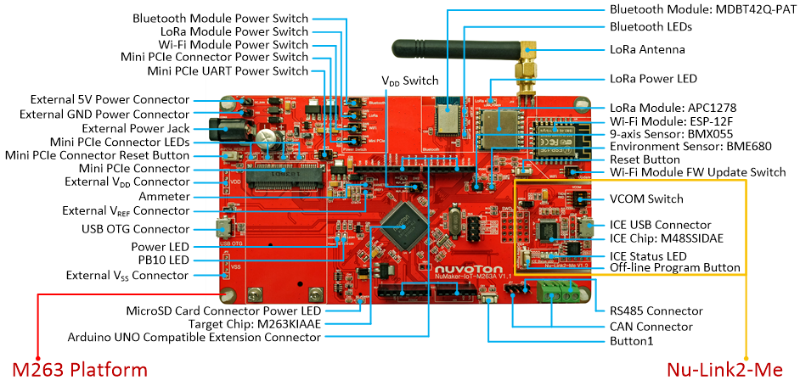
\includegraphics[width=\linewidth]{M263A.png}
\caption{Nuvoton M263A (front) \cite{Nuvoton}}
\label{fig:m263A}
\end{figure}

\begin{figure}[!ht]
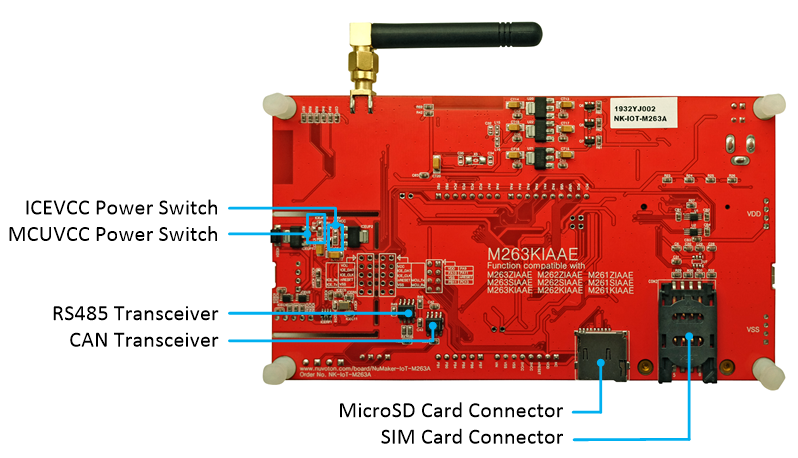
\includegraphics[width=\linewidth]{M263Aback.png}
\caption{Nuvoton M263A (back) \cite{Nuvoton}}
\label{fig:m263Aback}
\end{figure}

\begin{figure}[!ht]
\centering
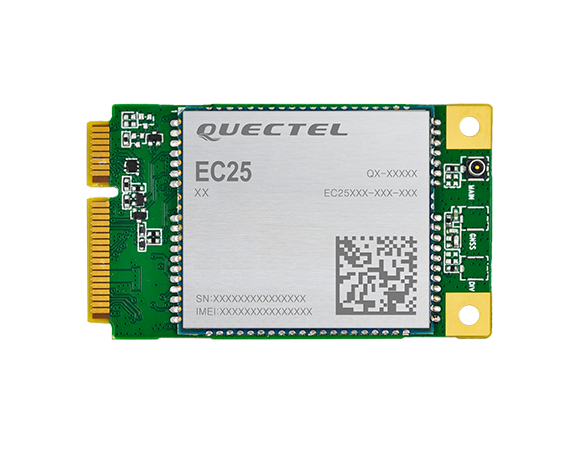
\includegraphics[width=0.5\linewidth]{ec25.png}
\caption{Quectel EC25 \cite{Quectel}}
\label{fig:quectelEC25}
\end{figure}

\begin{figure}[!ht]
\centering
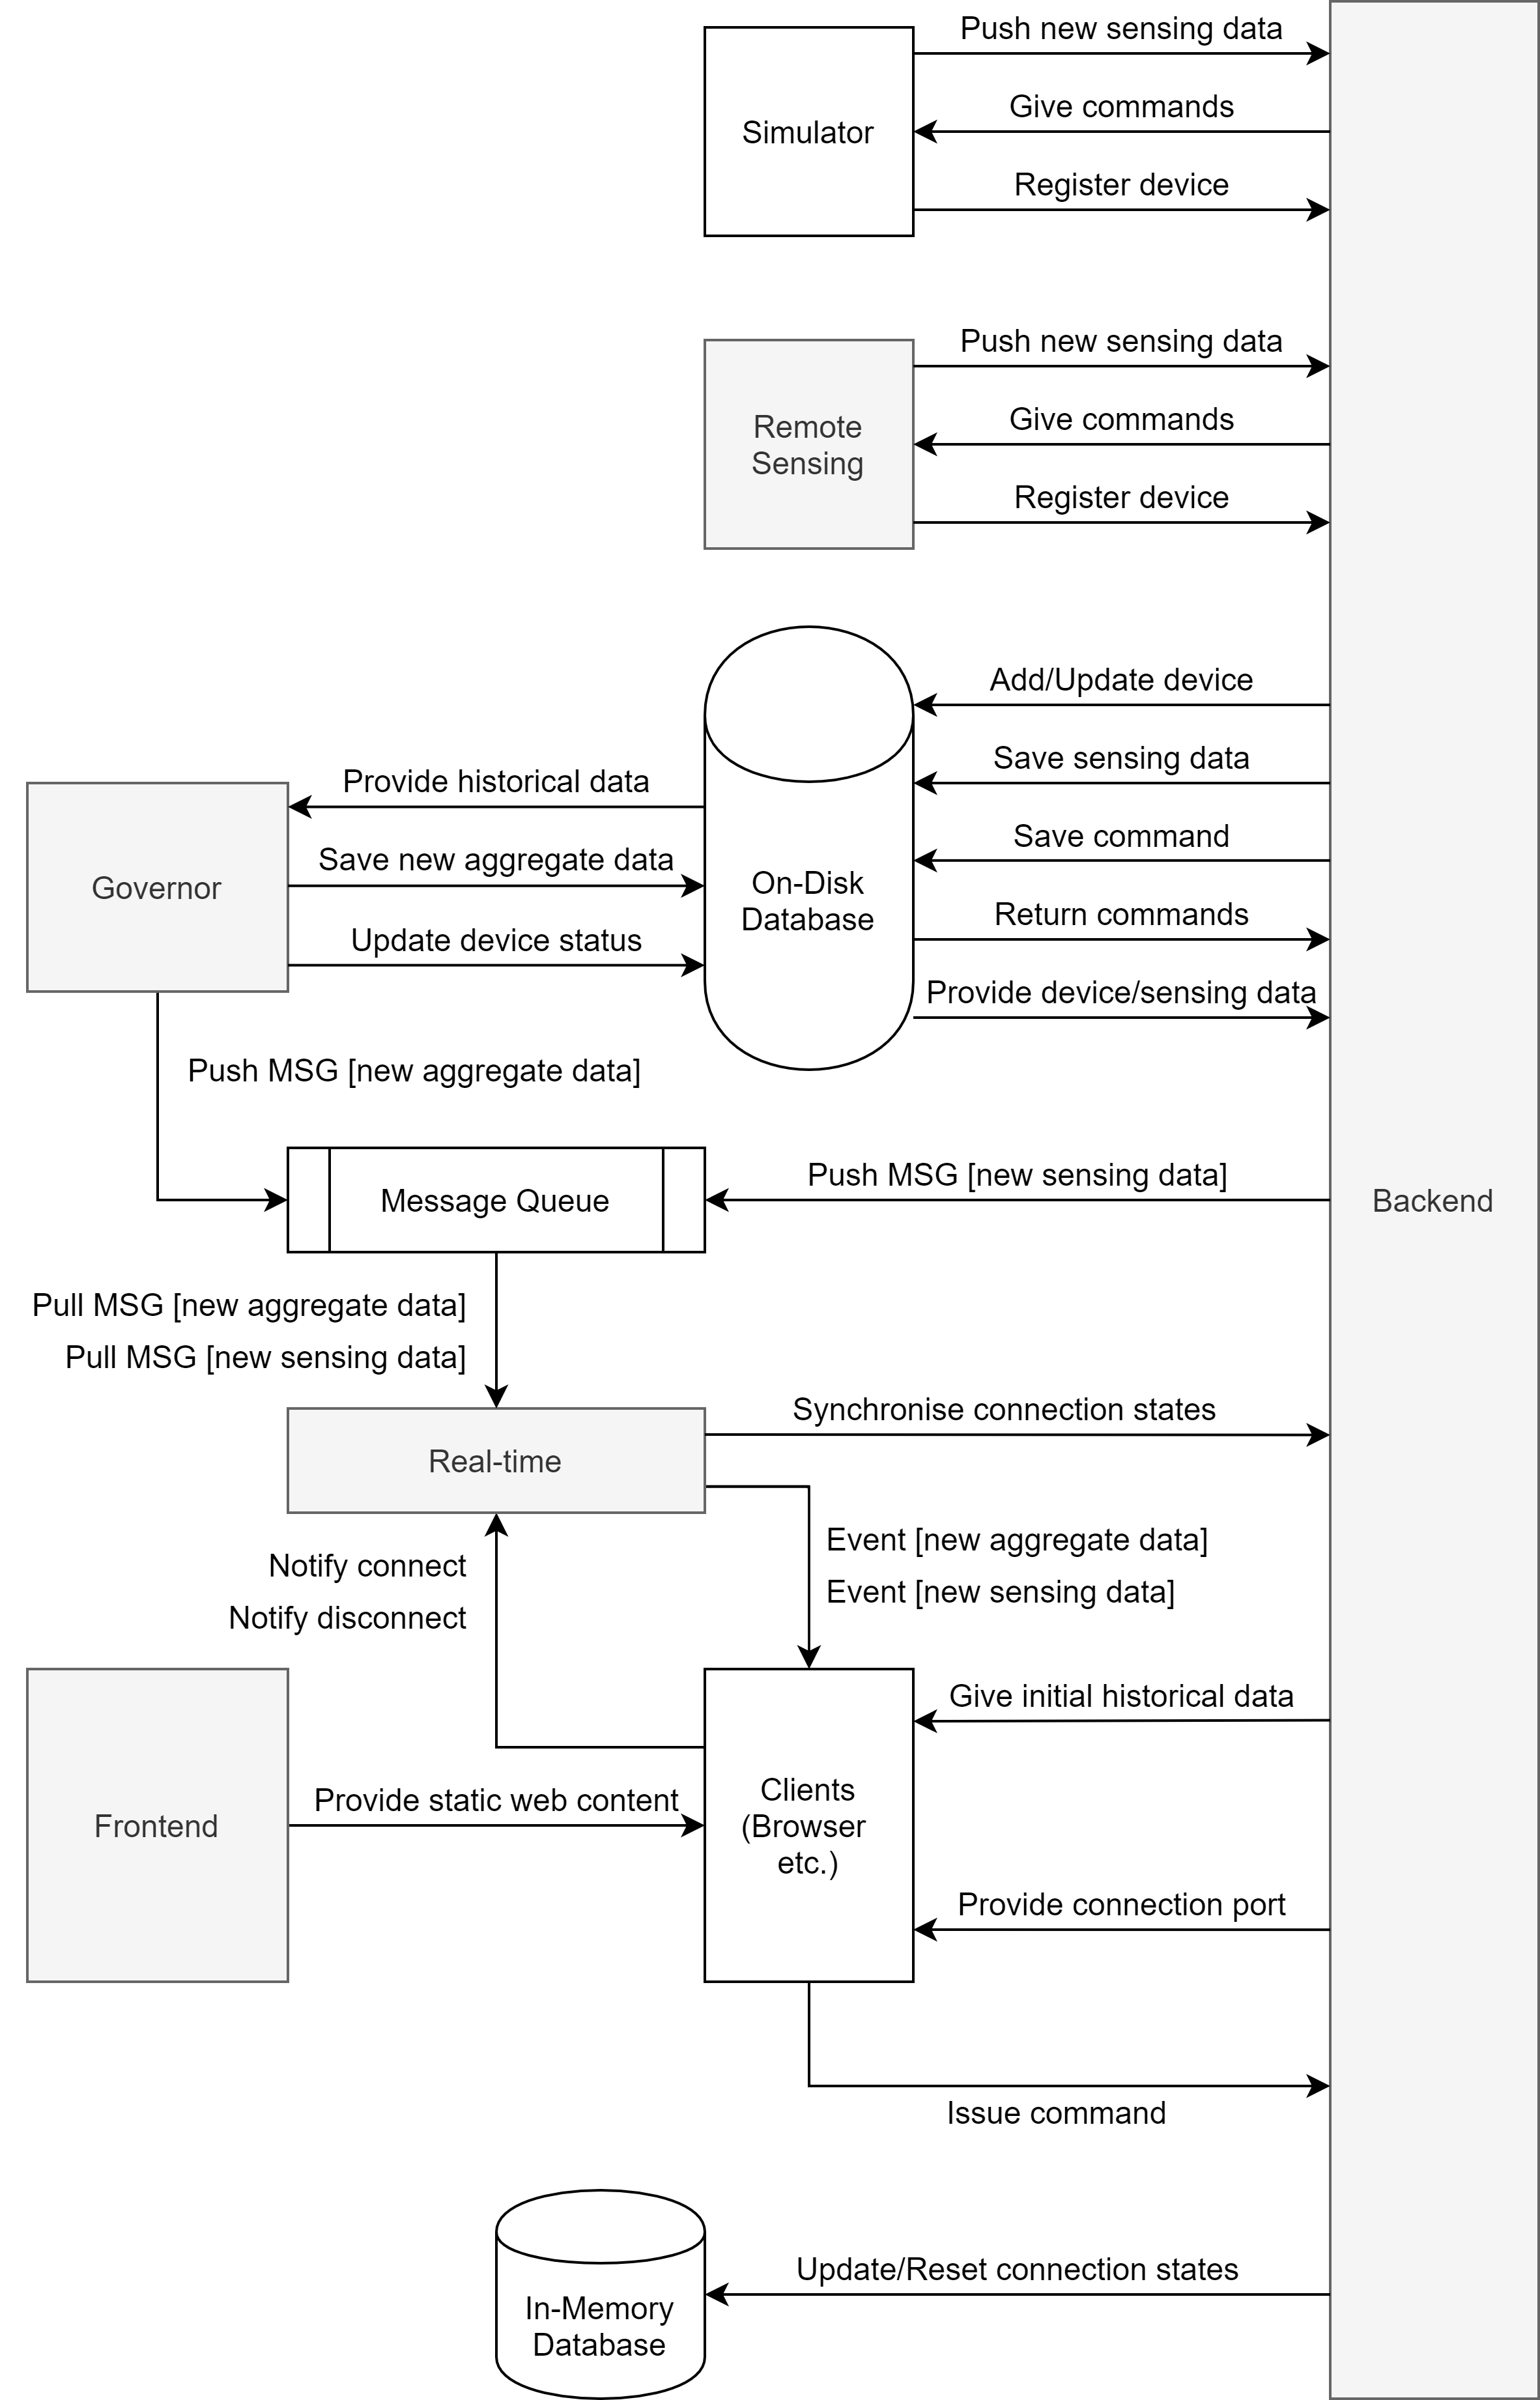
\includegraphics[width=\linewidth]{c4-toplevel.png}
\caption{Top-level architecture of the proposed system.}
\label{fig:toplevel}
\end{figure}

\begin{figure}[!ht]
\centering
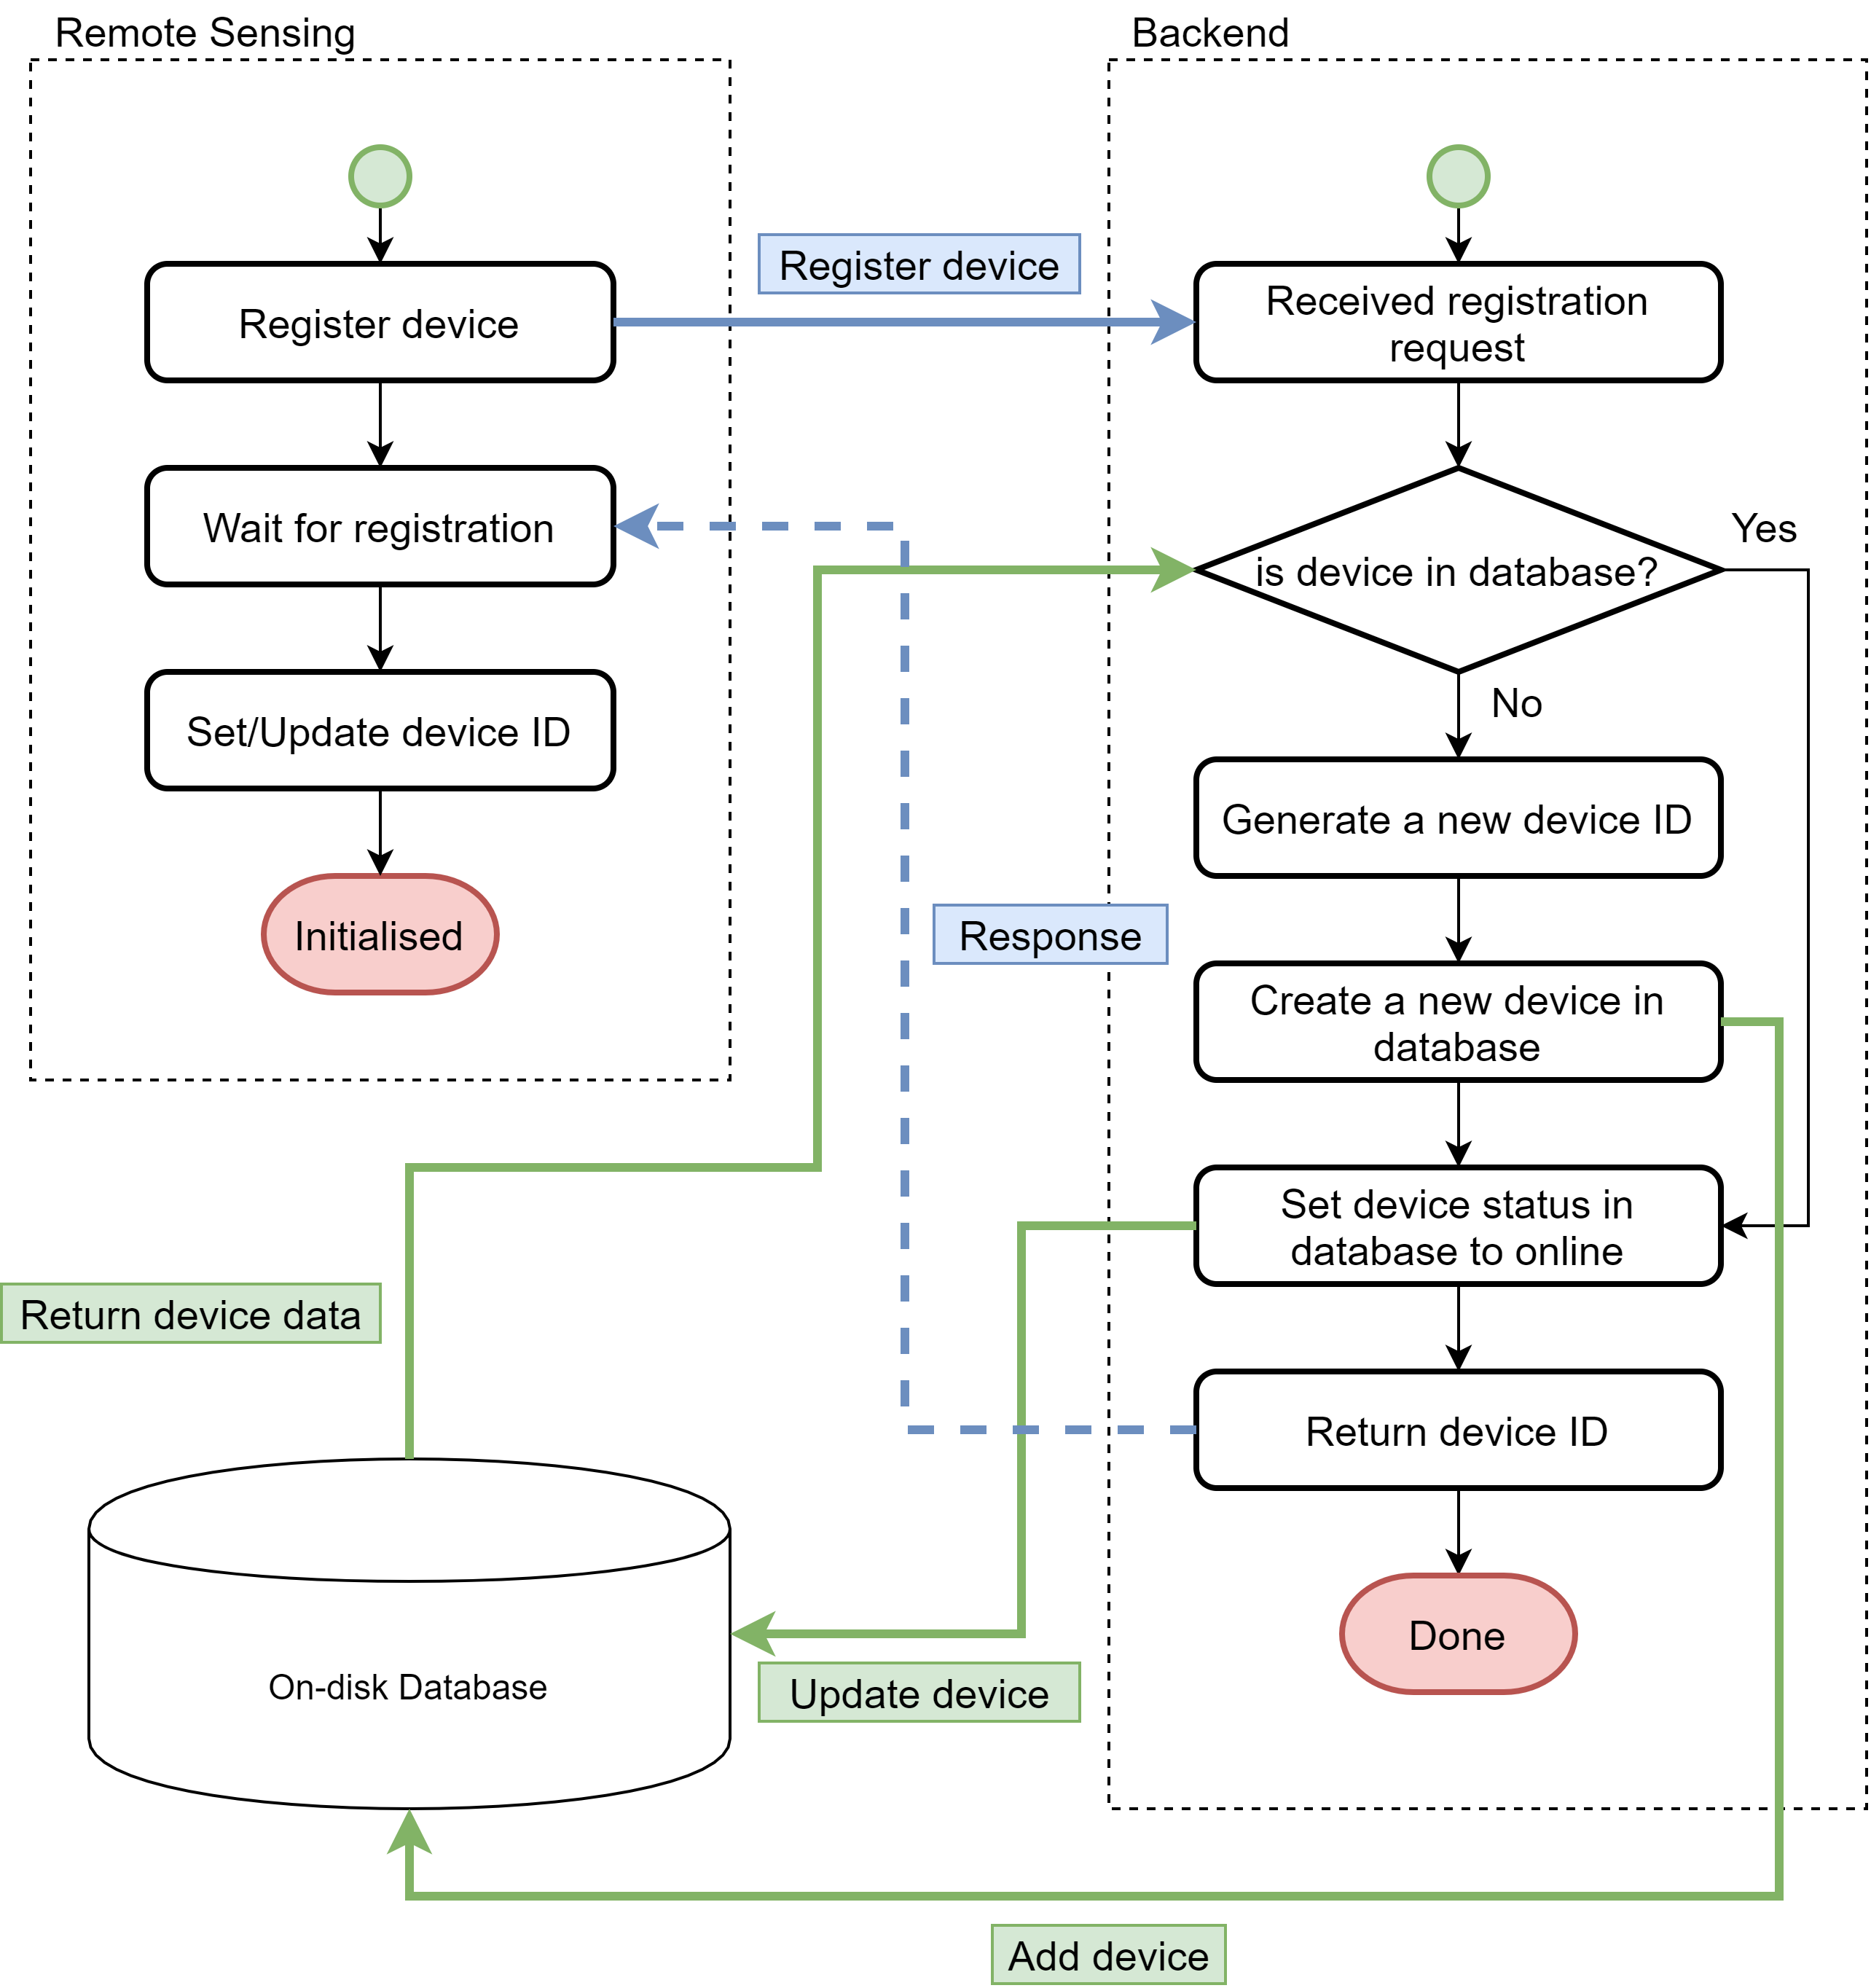
\includegraphics[width=\linewidth]{c4-initialisation.png}
\caption{The initialisation process.}
\label{fig:init}
\end{figure}

\begin{figure}[!ht]
\centering
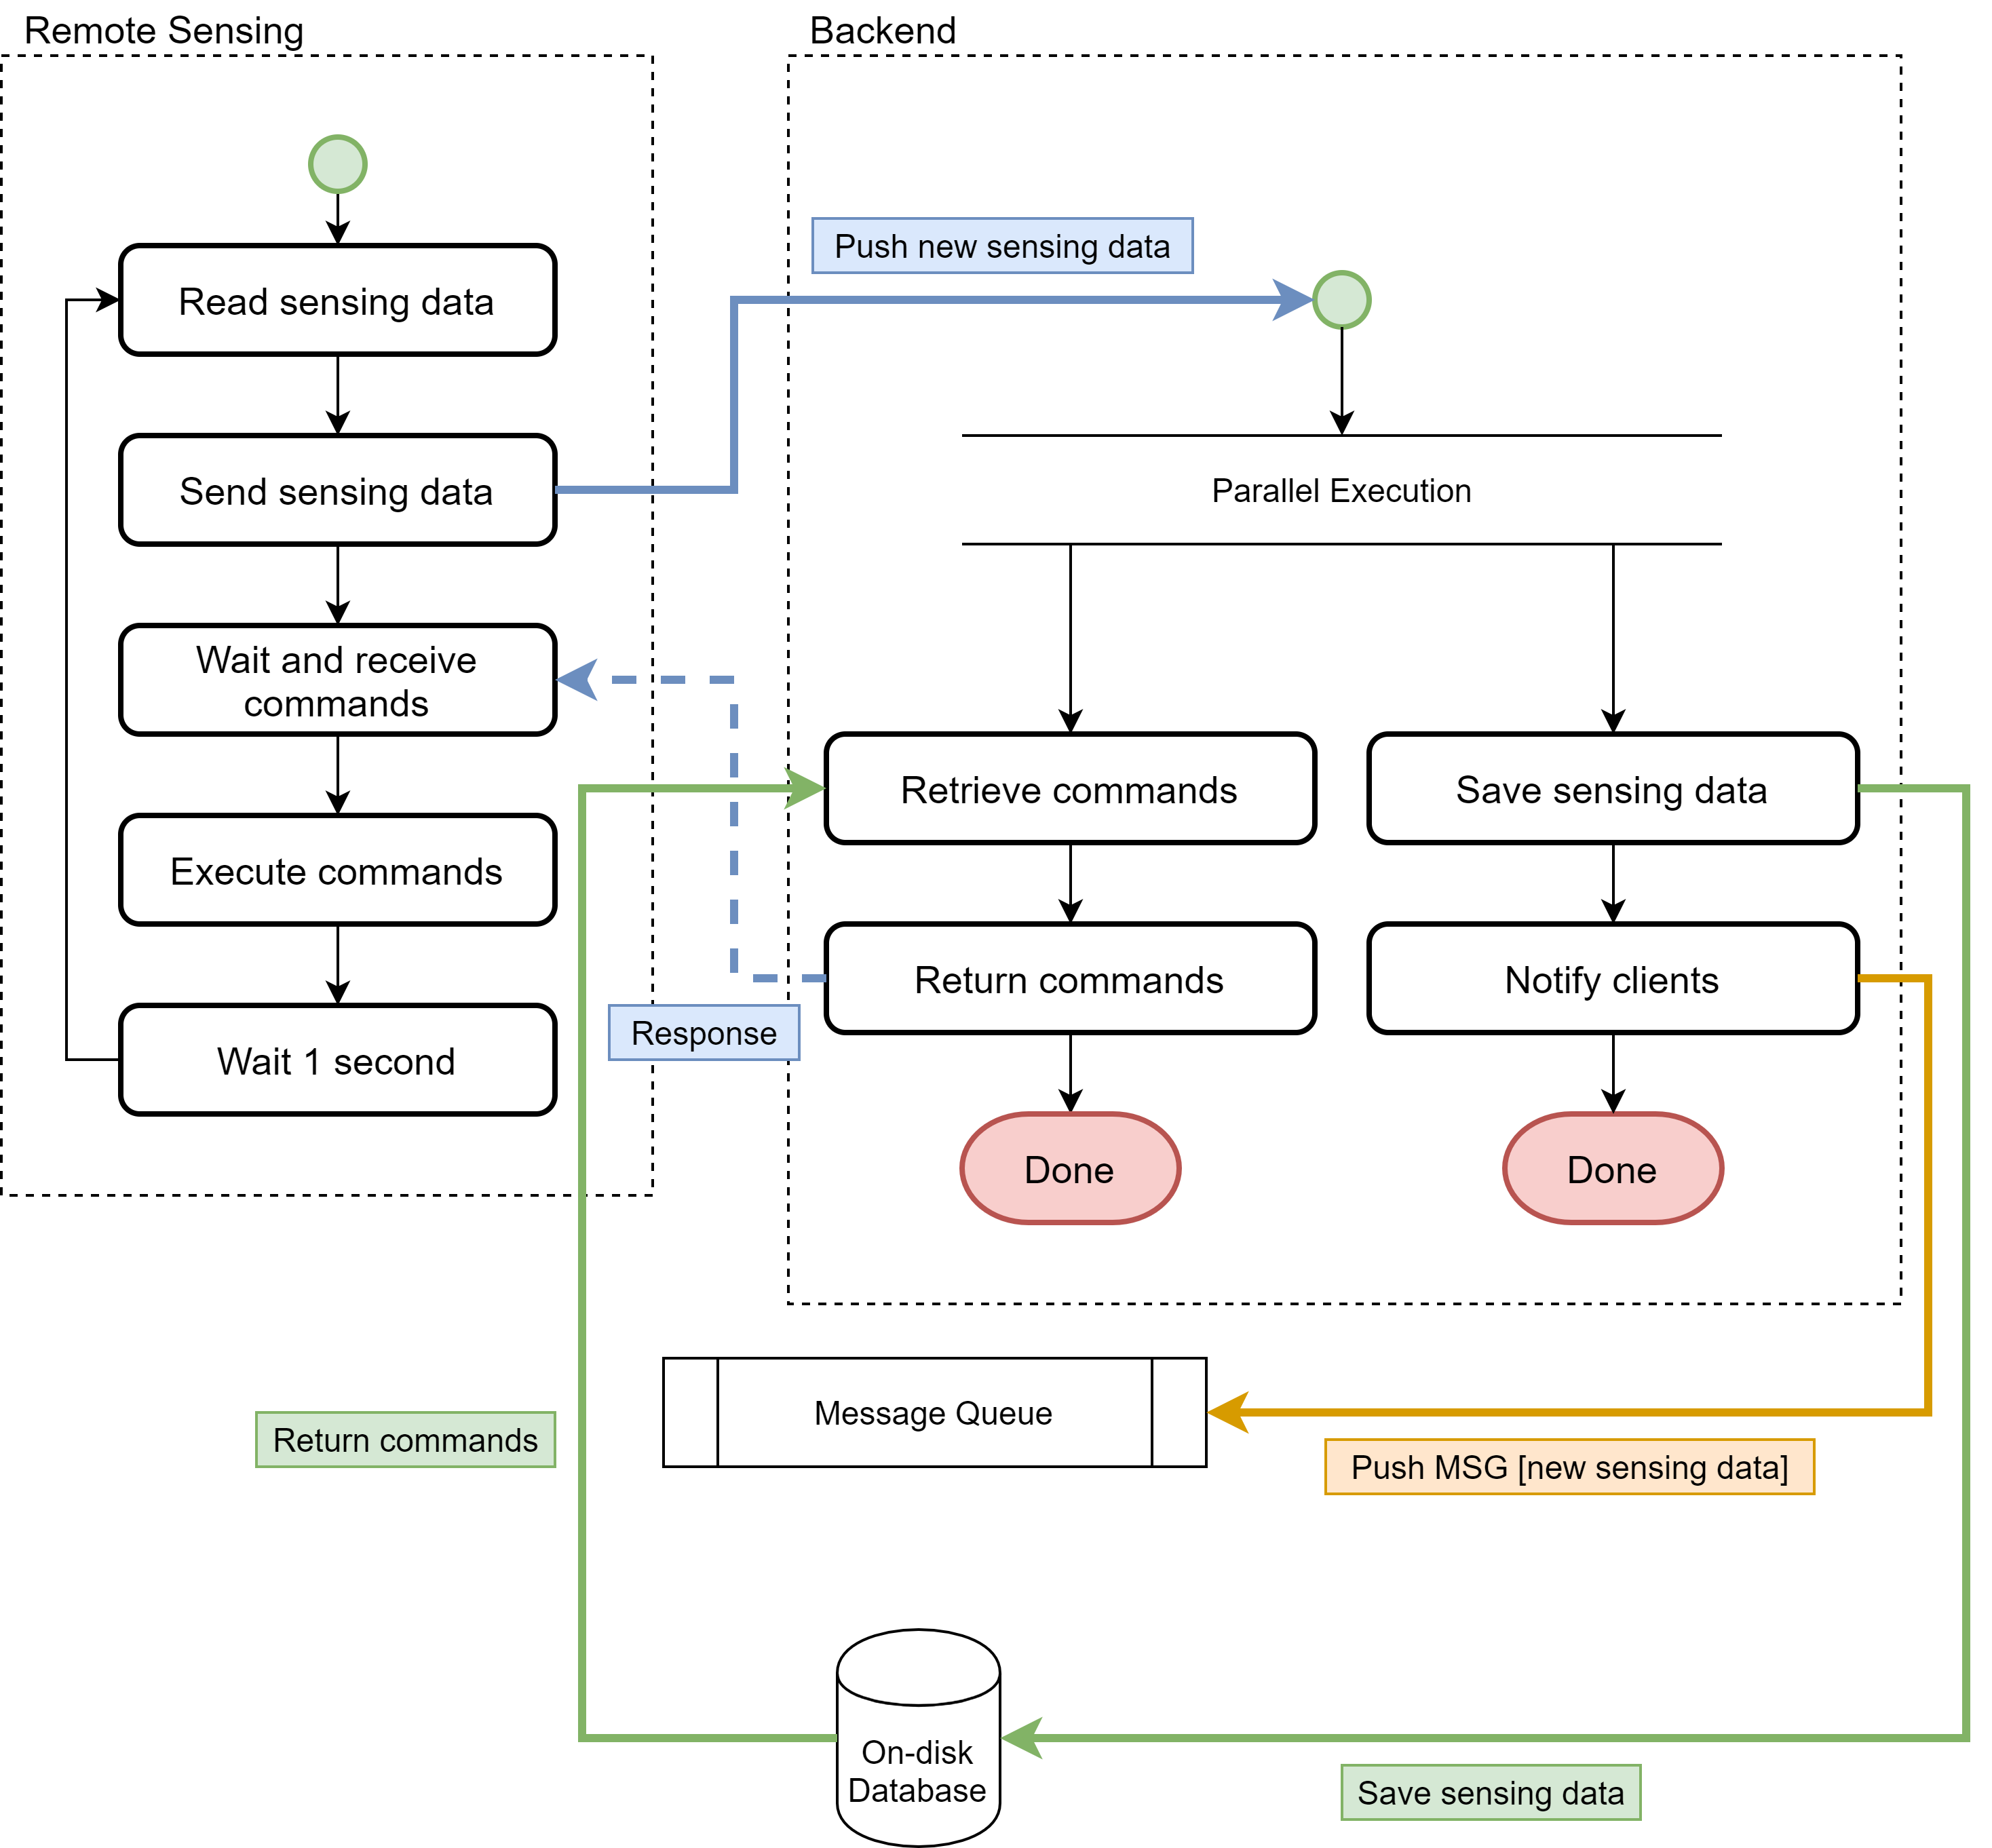
\includegraphics[width=\linewidth]{c4-recording.png}
\caption{The data recording and device controlling process.}
\label{fig:record}
\end{figure}

\begin{figure}[!ht]
\centering
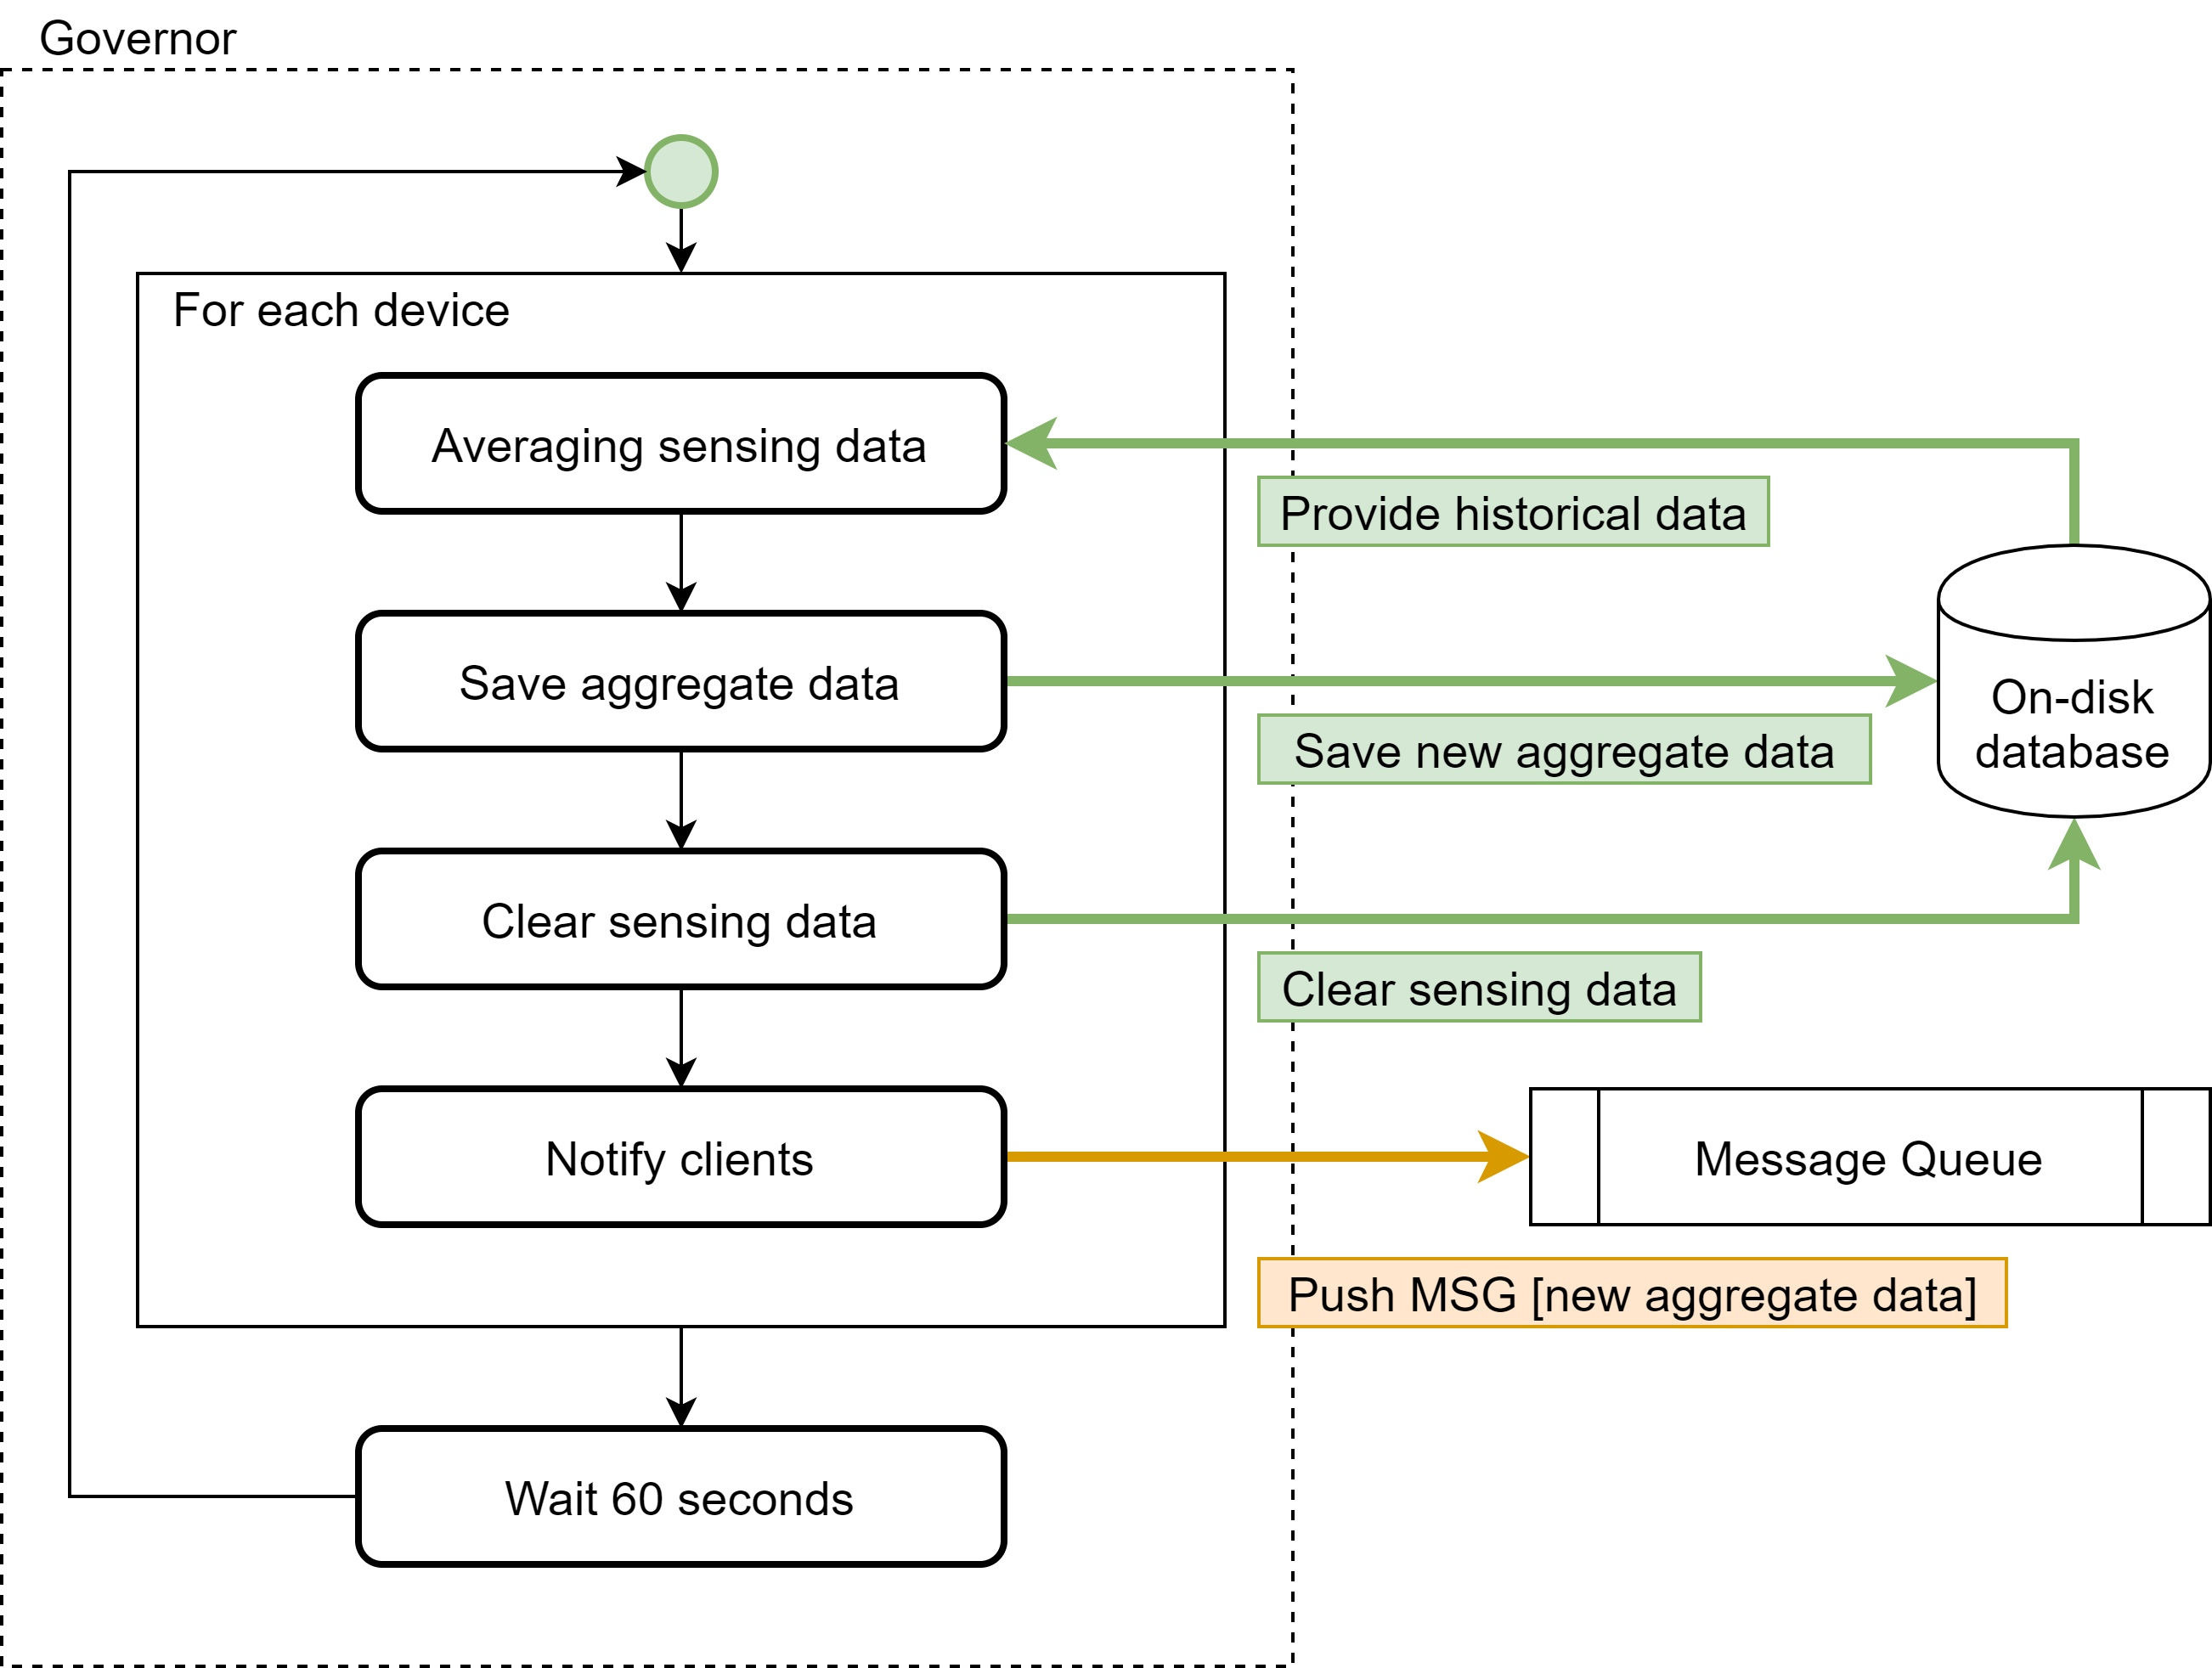
\includegraphics[width=\linewidth]{c4-governing.png}
\caption{The governing process.}
\label{fig:governing}
\end{figure}

\begin{figure}[!ht]
\centering
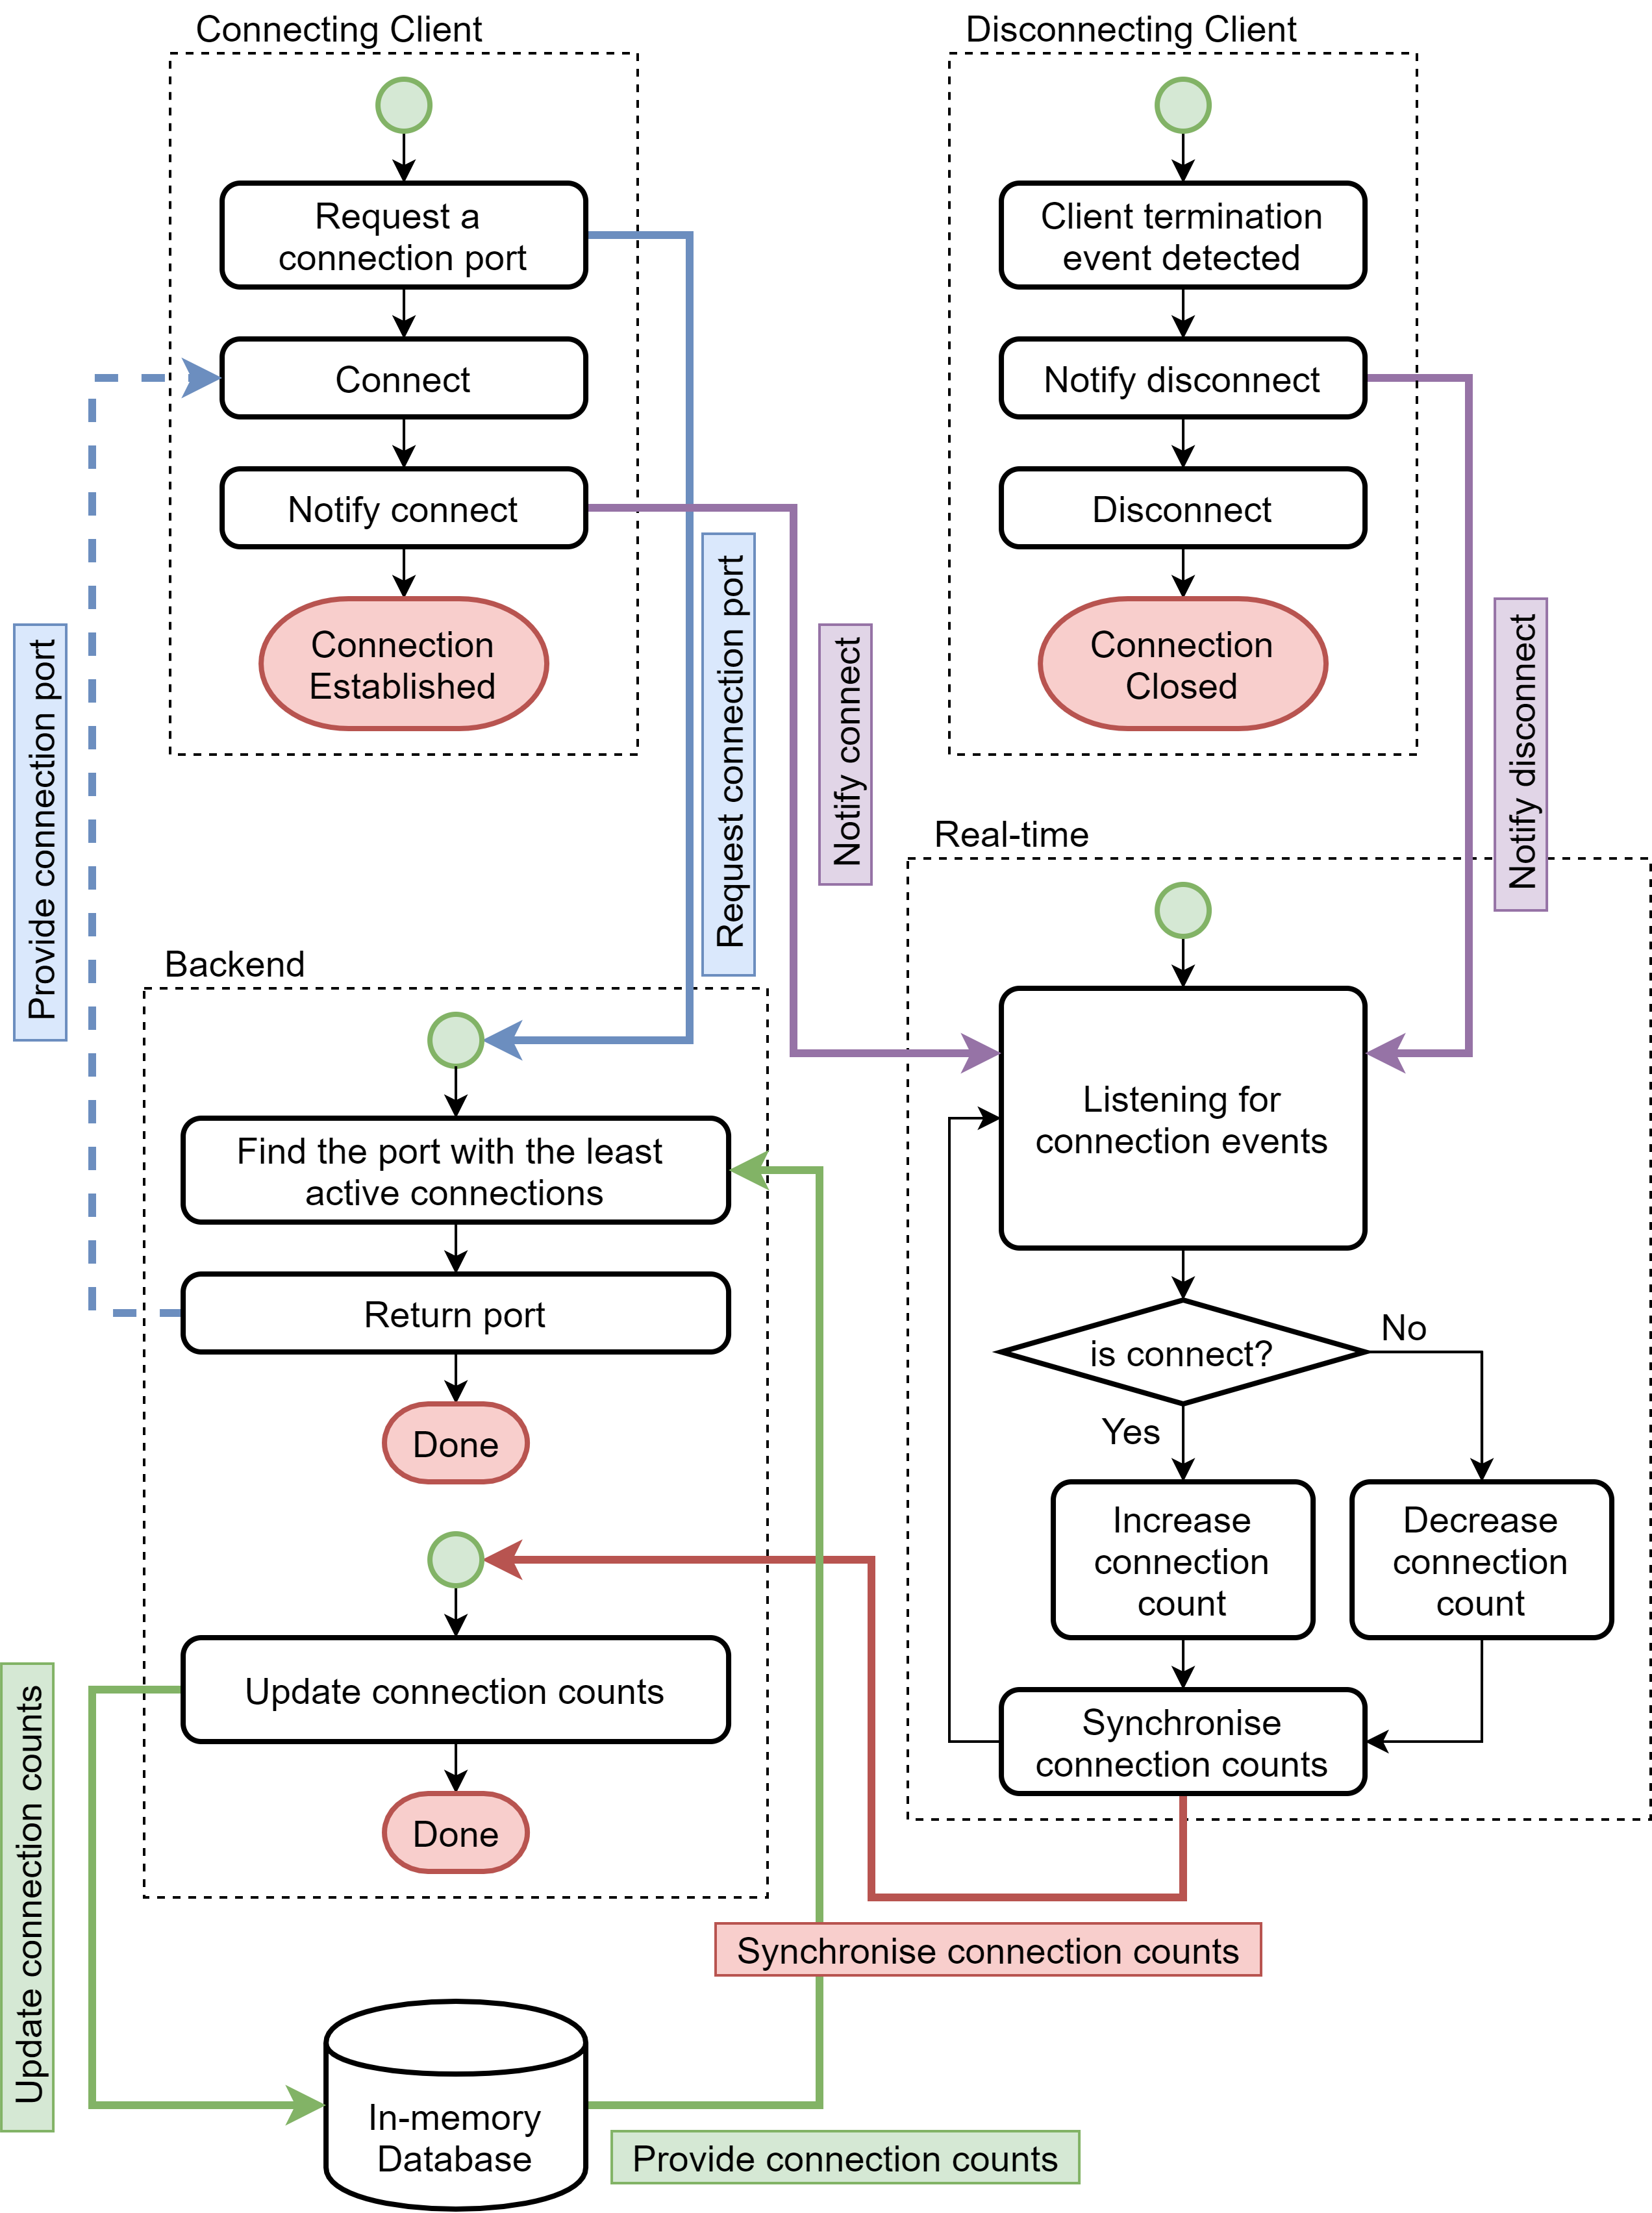
\includegraphics[width=0.95\linewidth]{c4-loadbalance.png}
\caption{The context-aware load balancing process.}
\label{fig:loadbalancing}
\end{figure}

\begin{figure}[!ht]
\centering
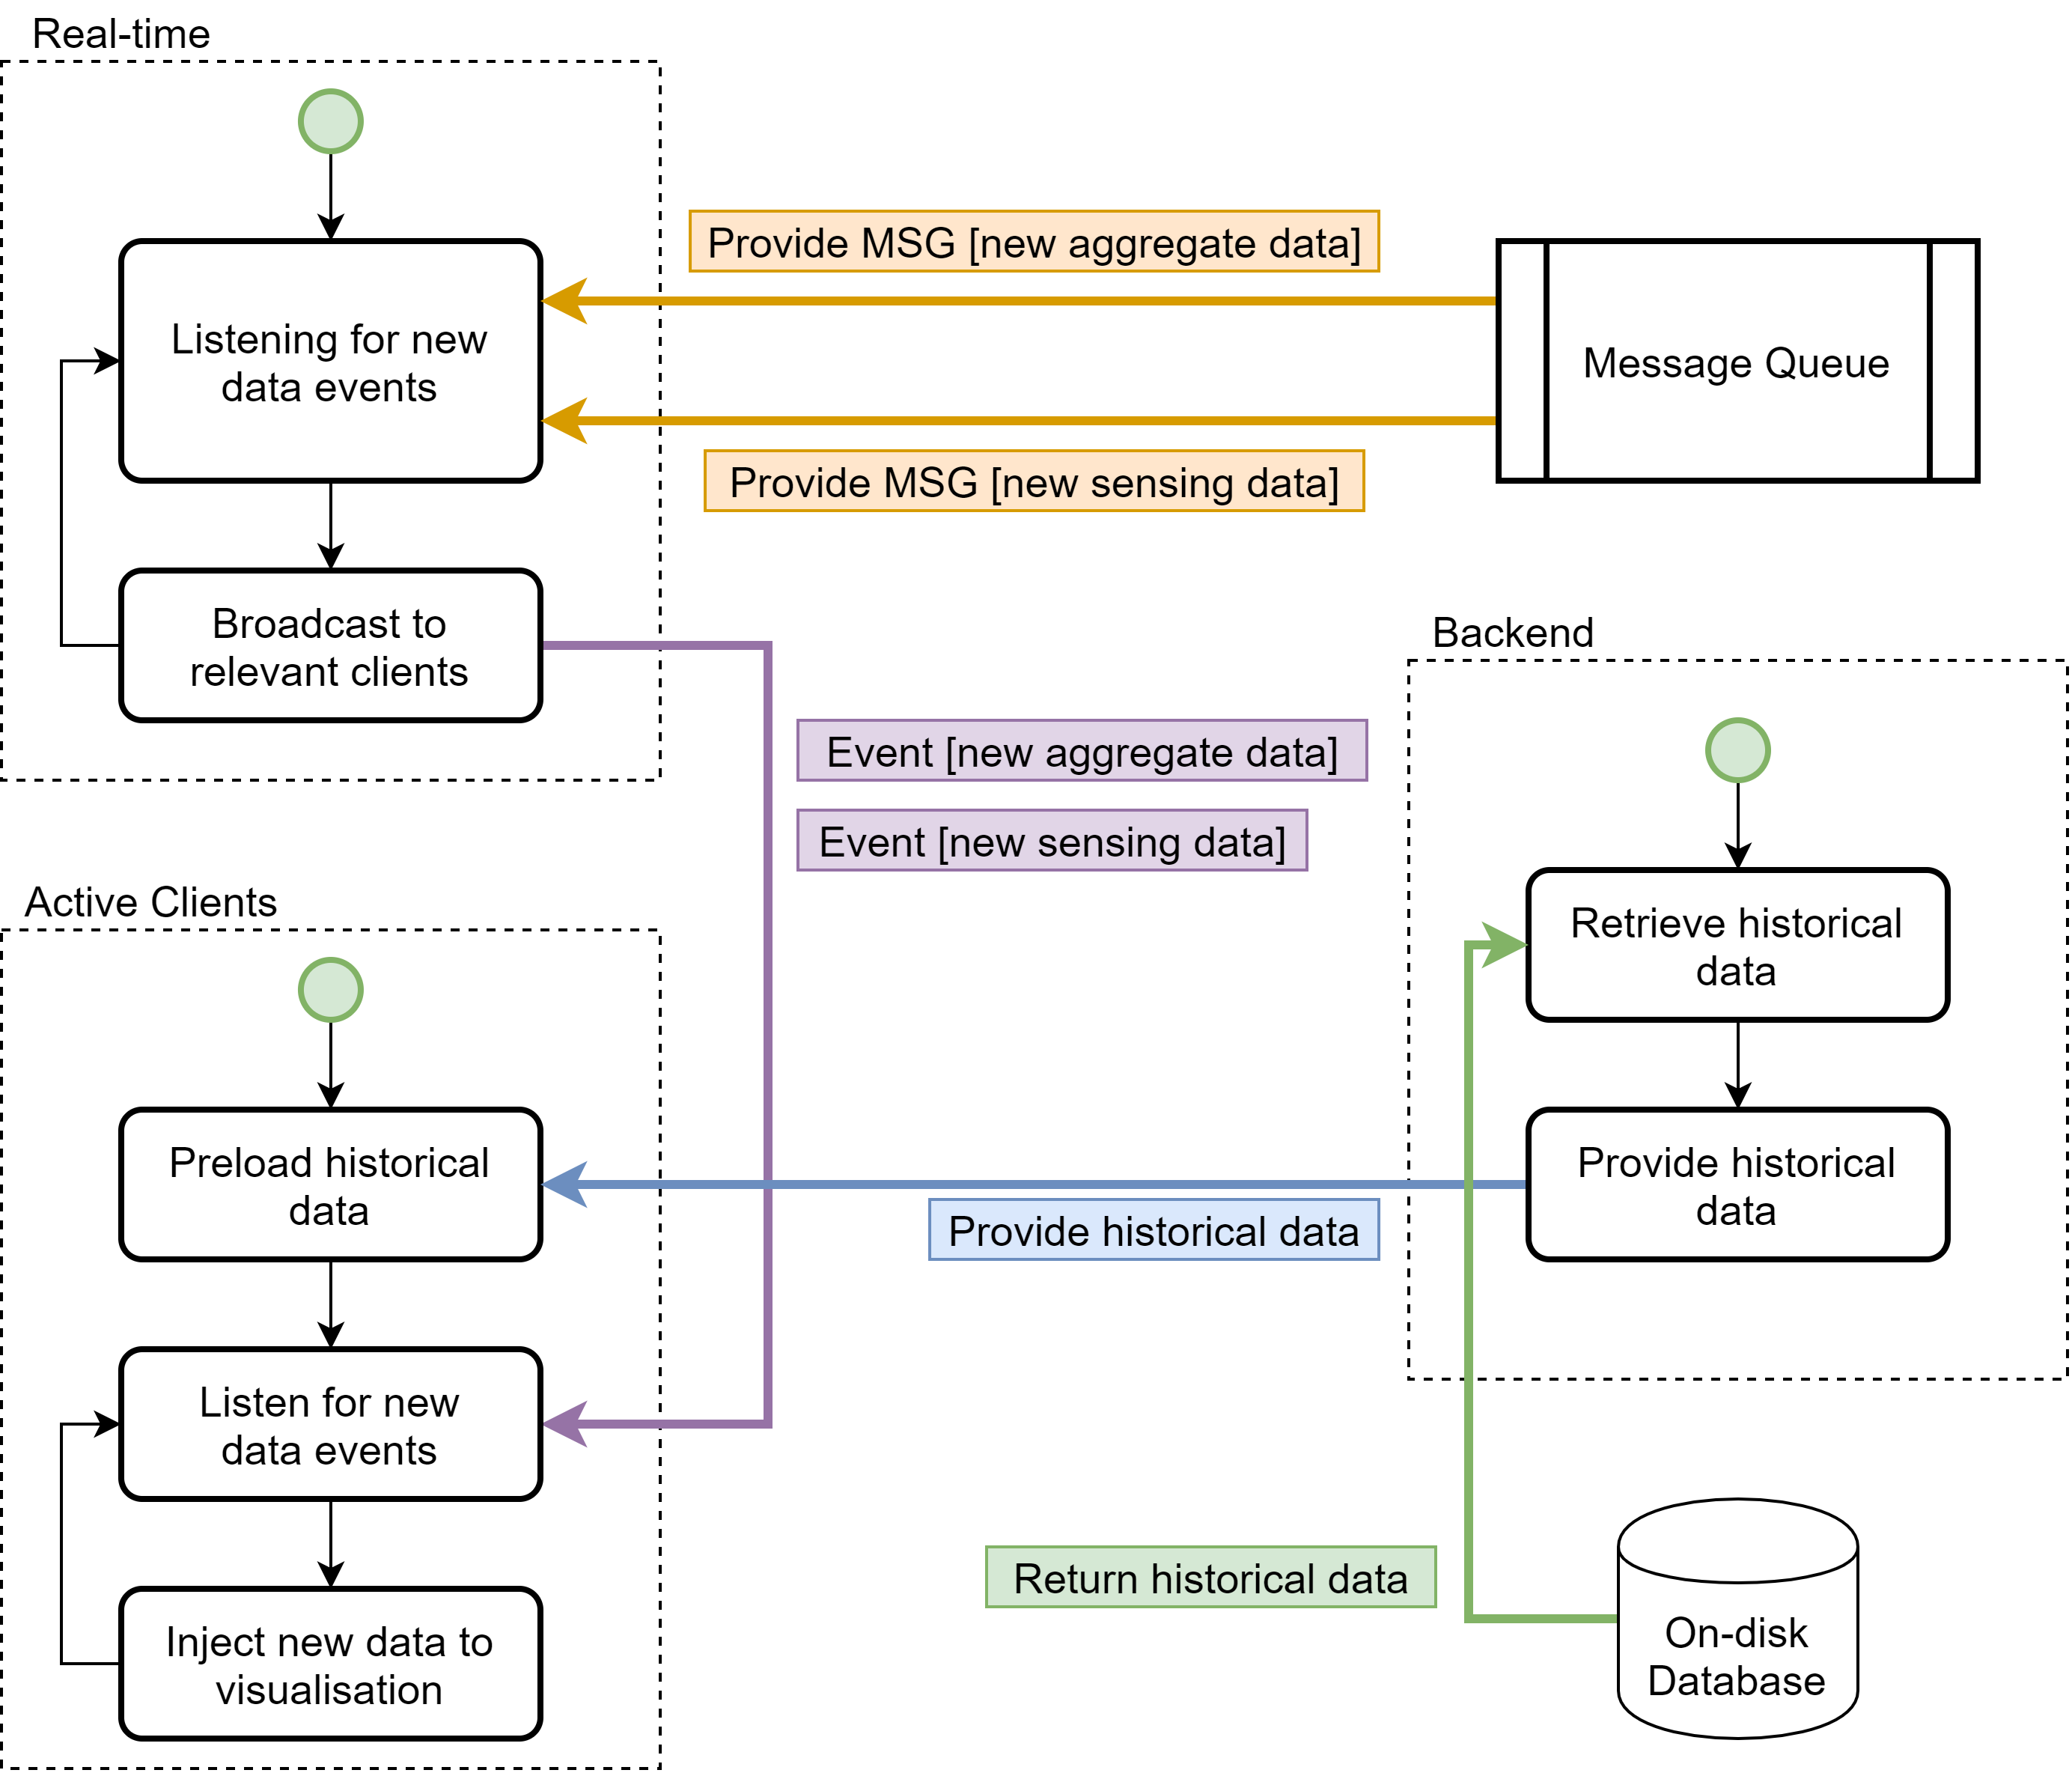
\includegraphics[width=\linewidth]{c4-monitoring.png}
\caption{The data monitoring process.}
\label{fig:monitoring}
\end{figure}

\begin{figure}[!ht]
\centering
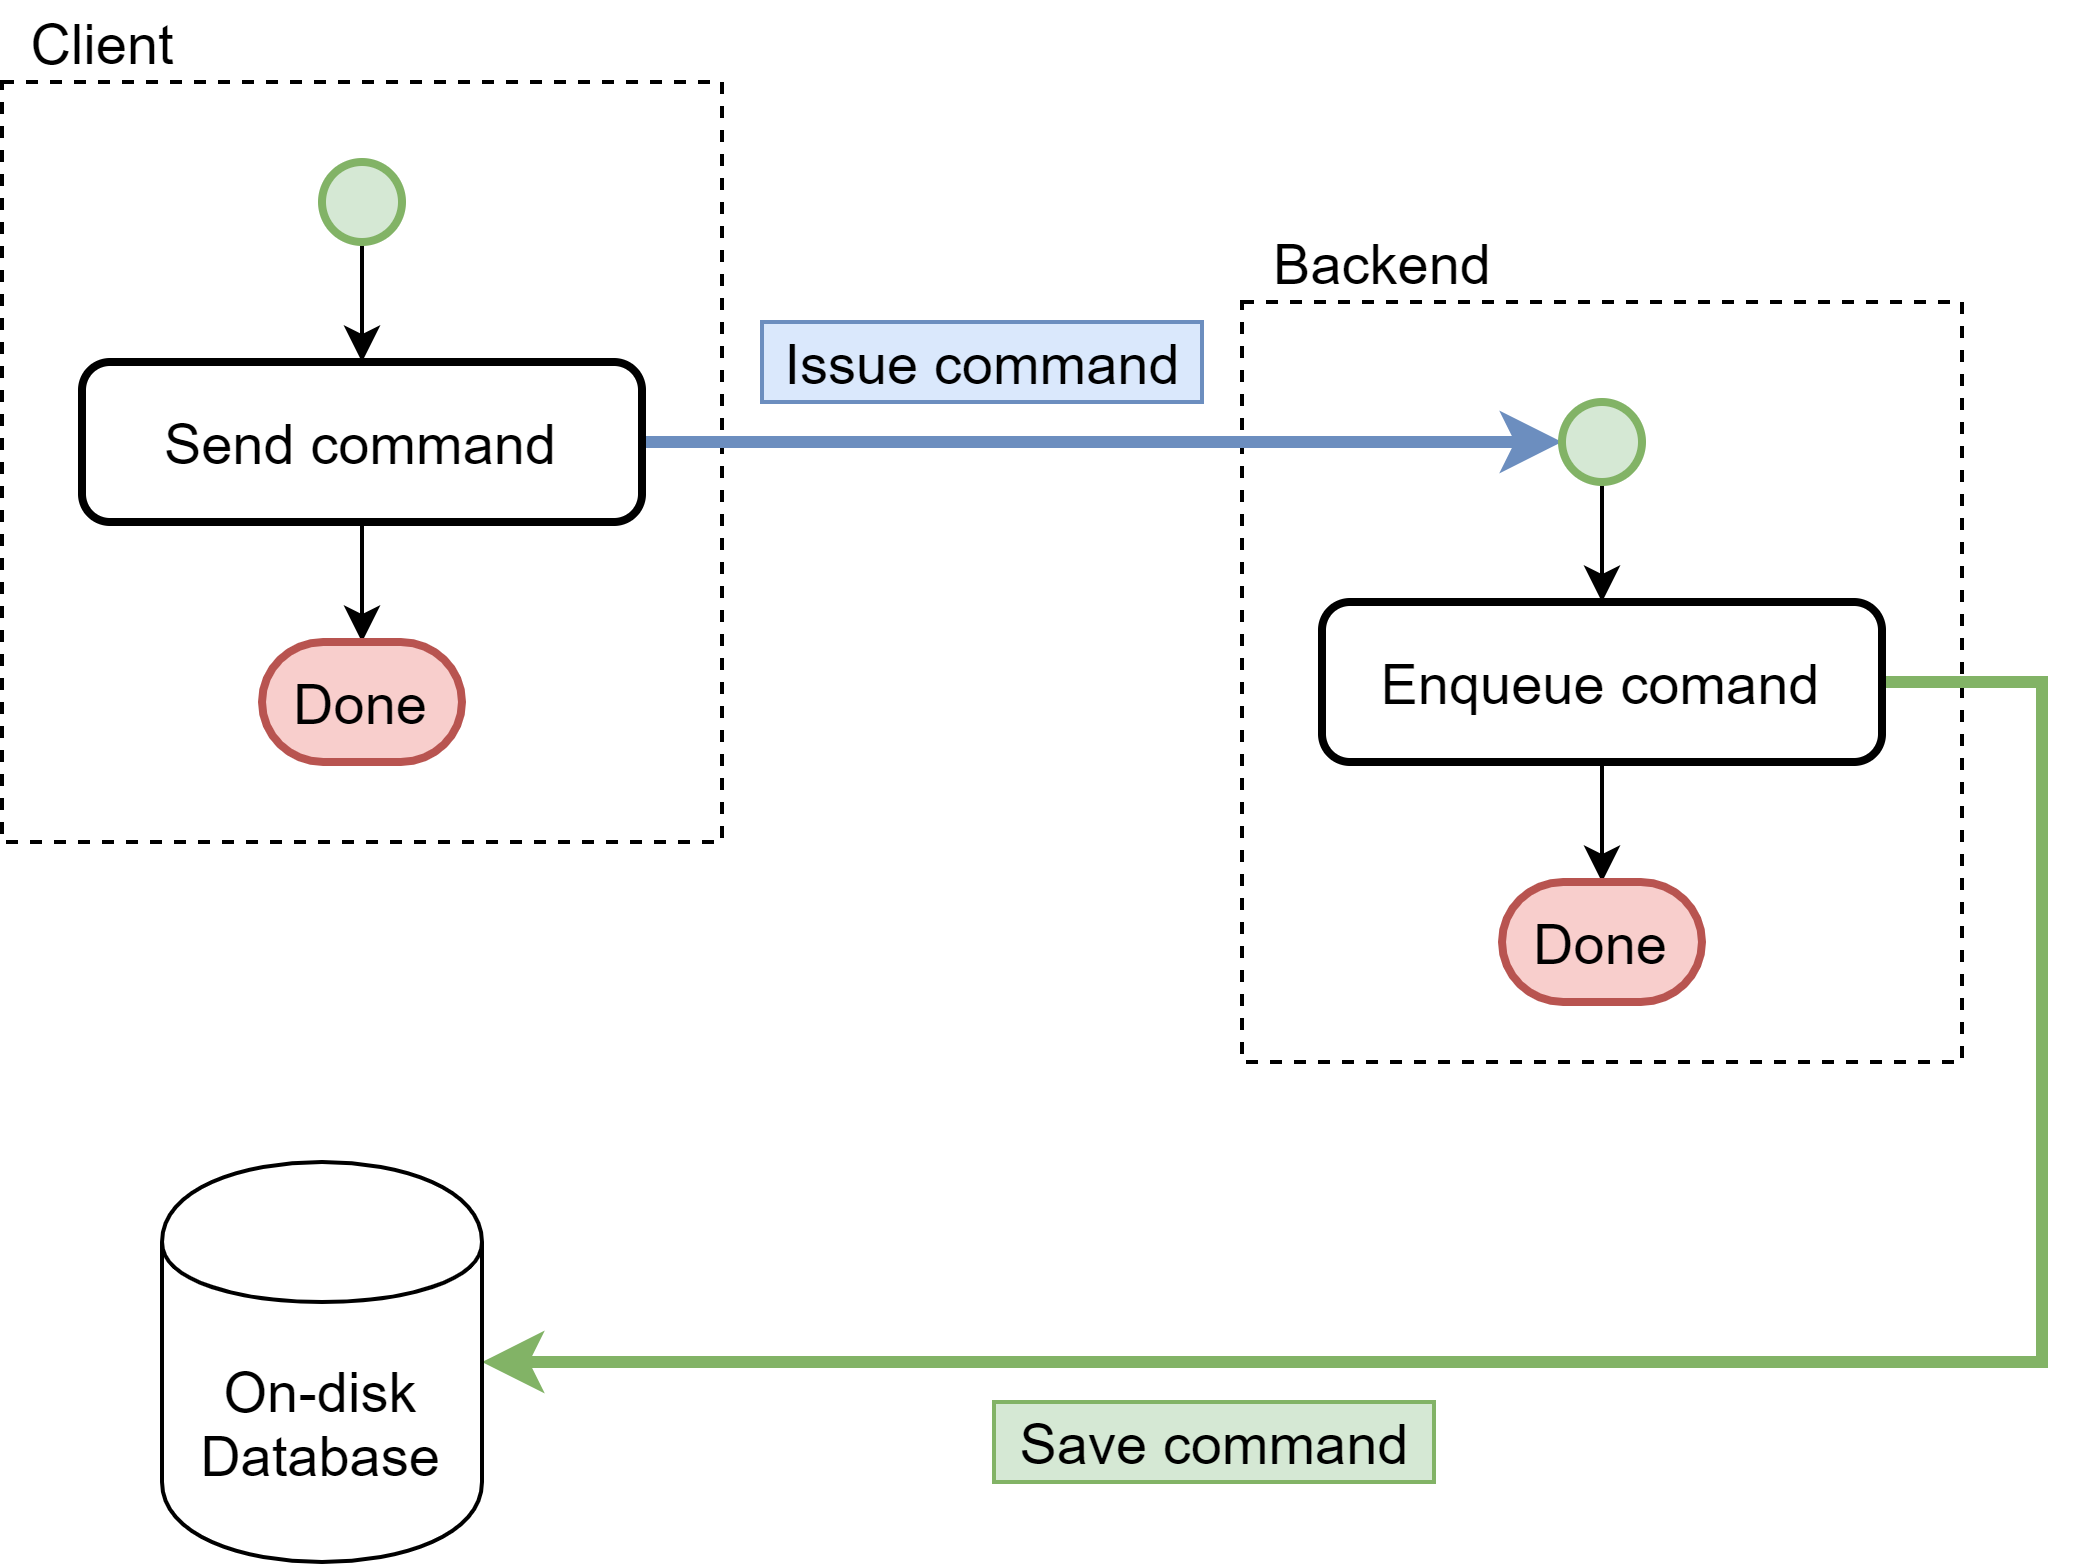
\includegraphics[width=\linewidth]{c4-issuing.png}
\caption{The process of issuing a command.}
\label{fig:issuing}
\end{figure}

\begin{figure}[!ht]
\centering
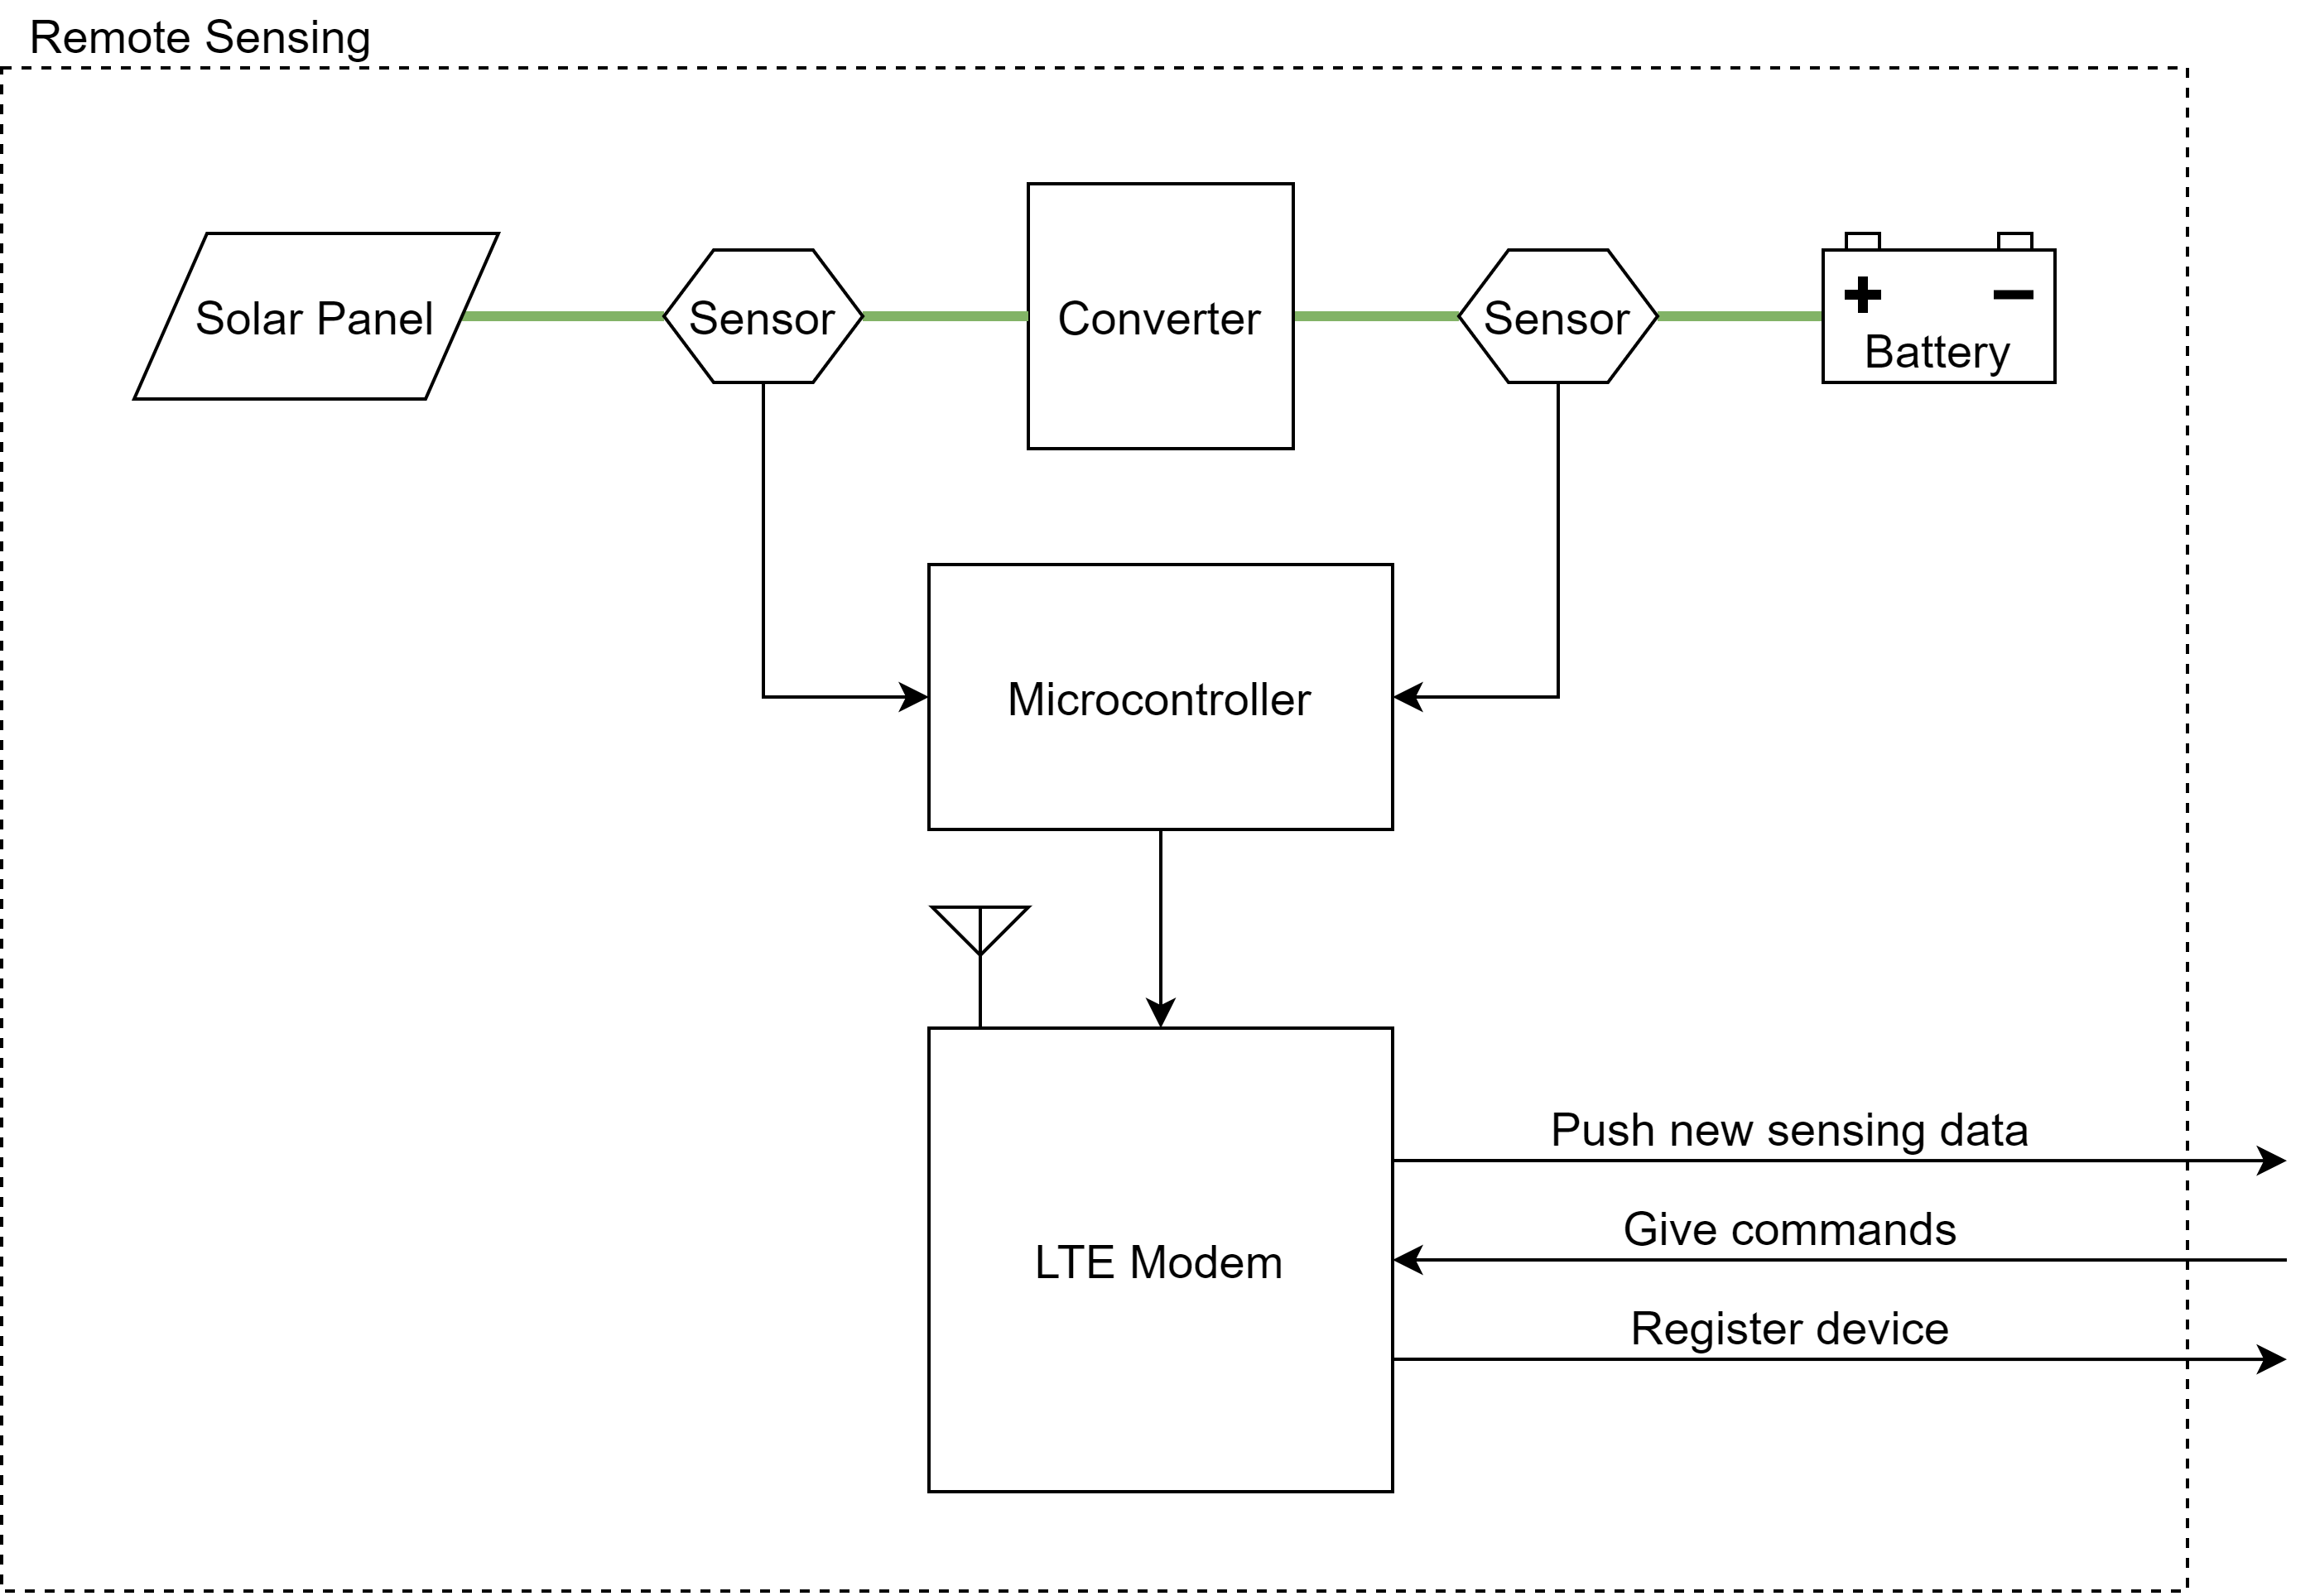
\includegraphics[width=\linewidth]{c4-sensing.png}
\caption{The architecture of the remote sensing composite component.}
\label{fig:sensing}
\end{figure}

\begin{figure}[!ht]
\centering
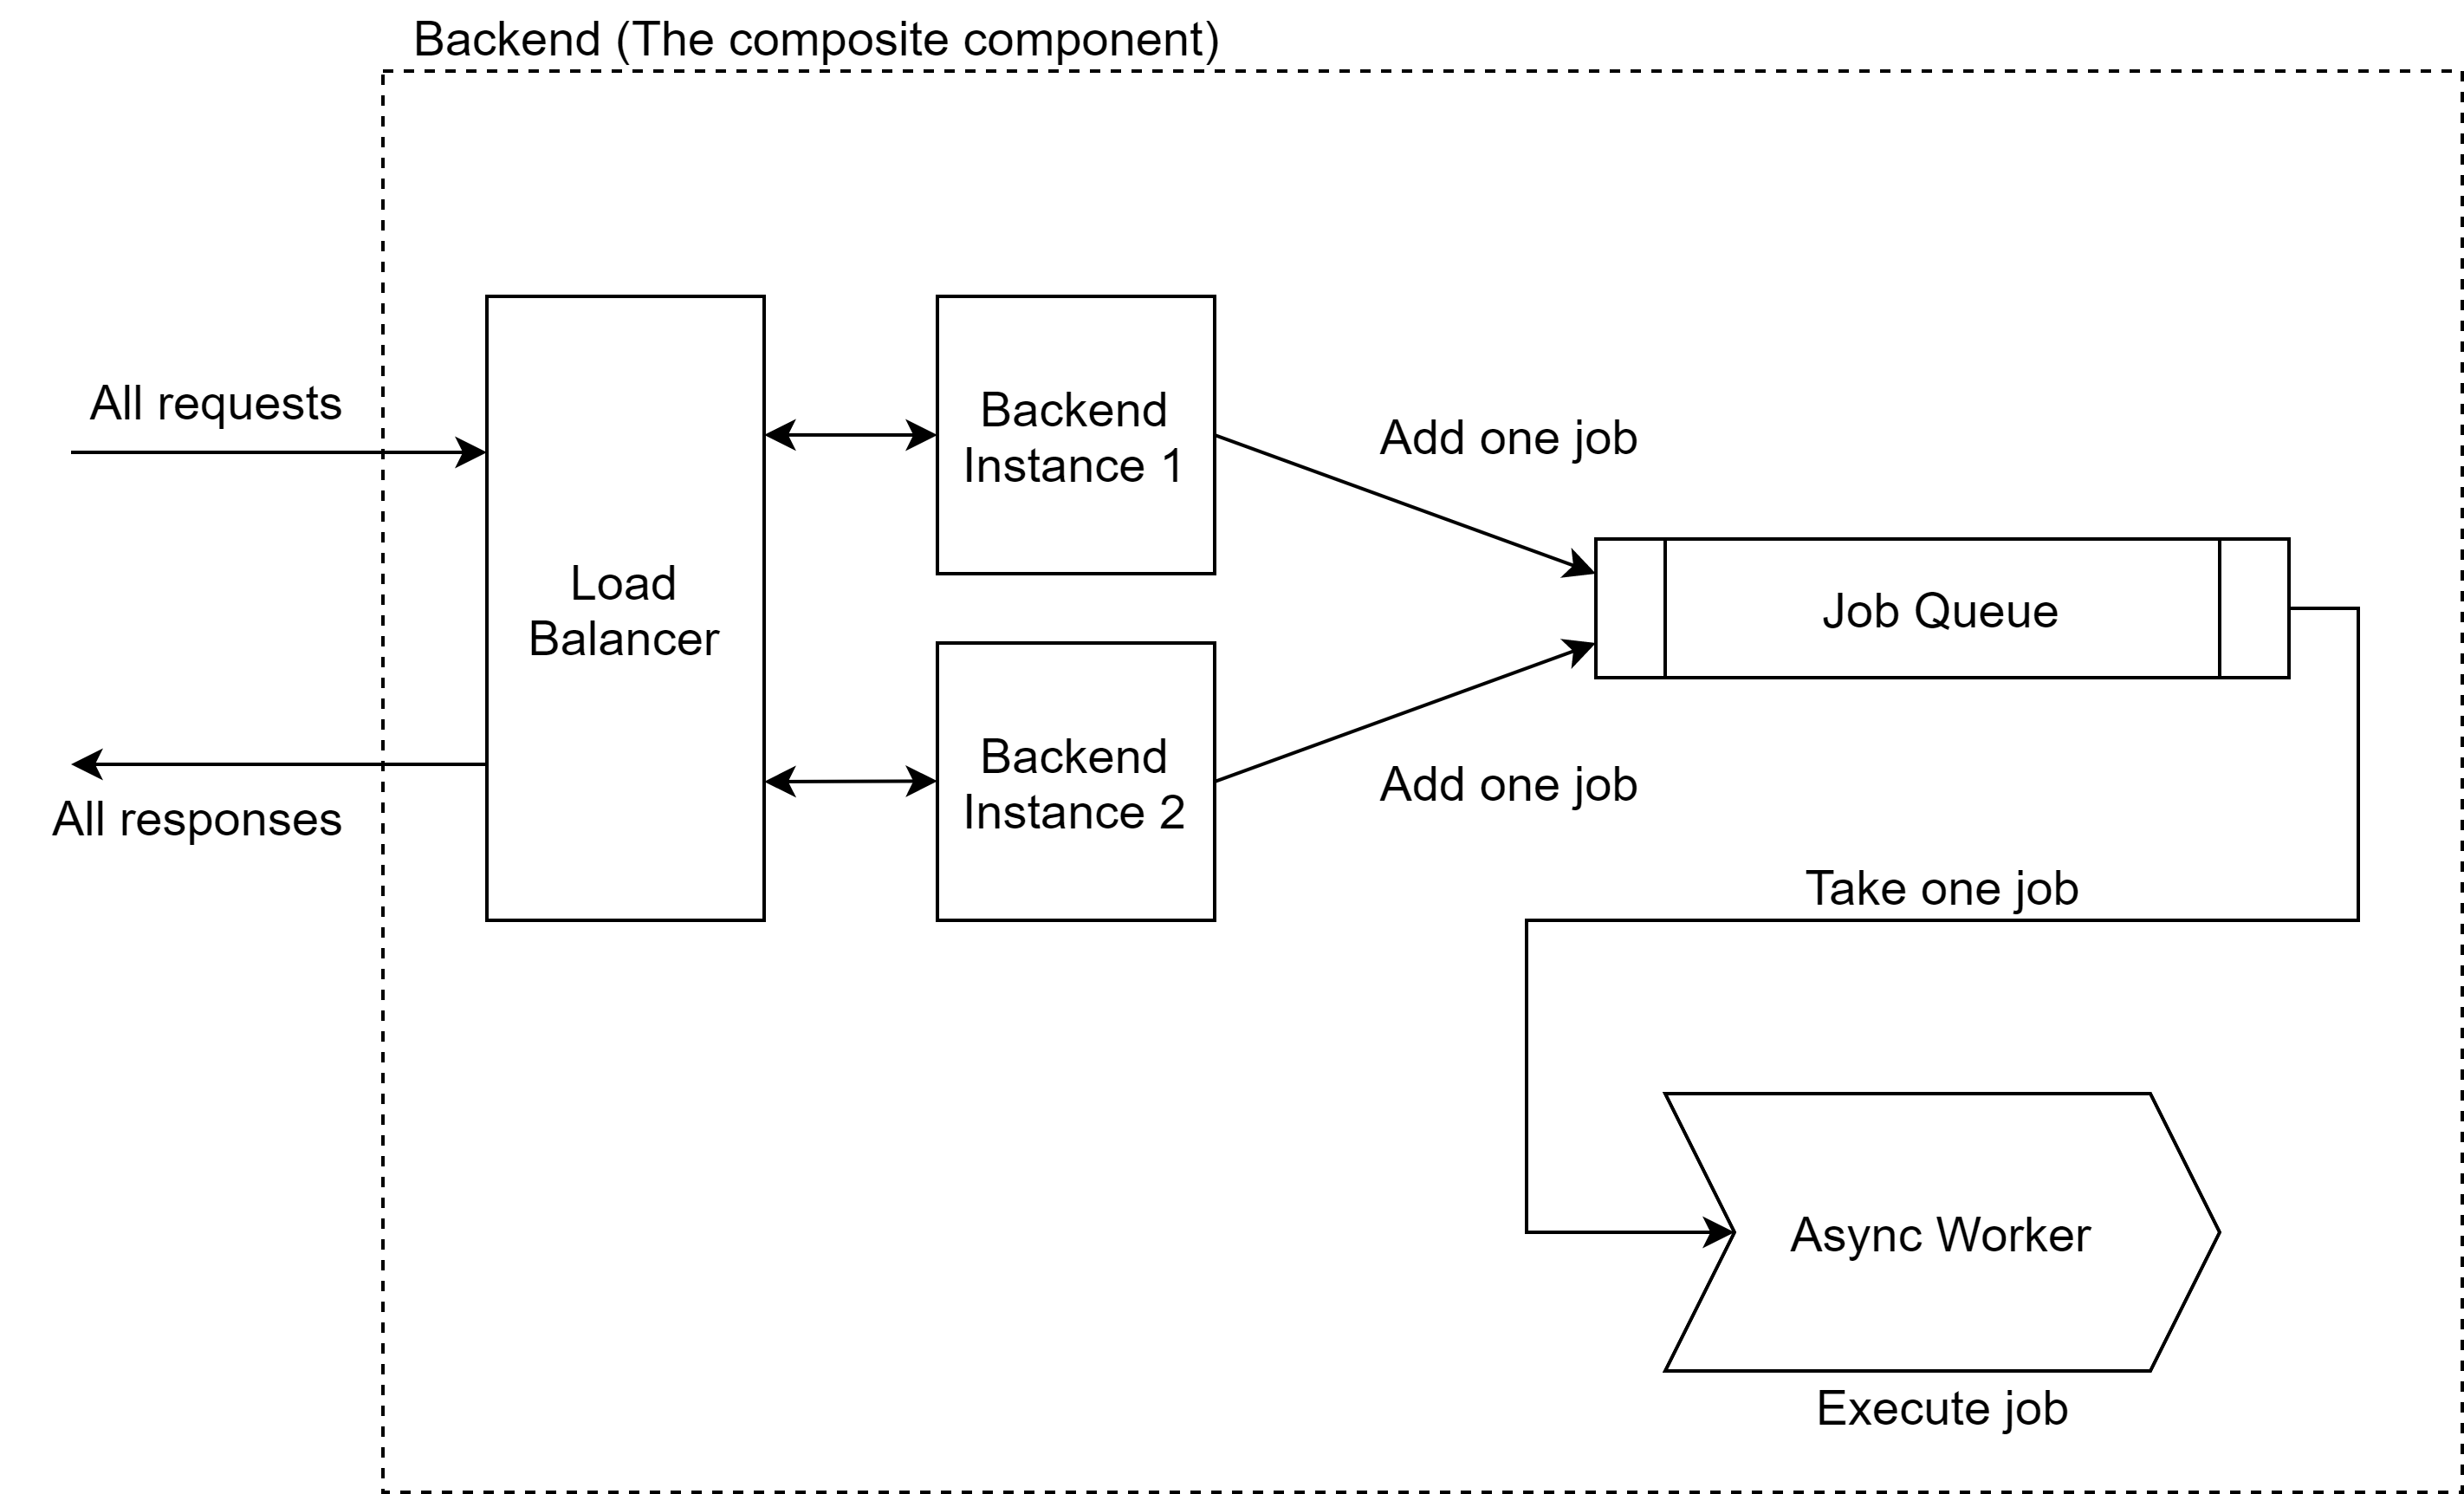
\includegraphics[width=\linewidth]{c4-backend.png}
\caption{The architecture of the backend composite component.}
\label{fig:backend}
\end{figure}

\begin{figure}[!ht]
\centering
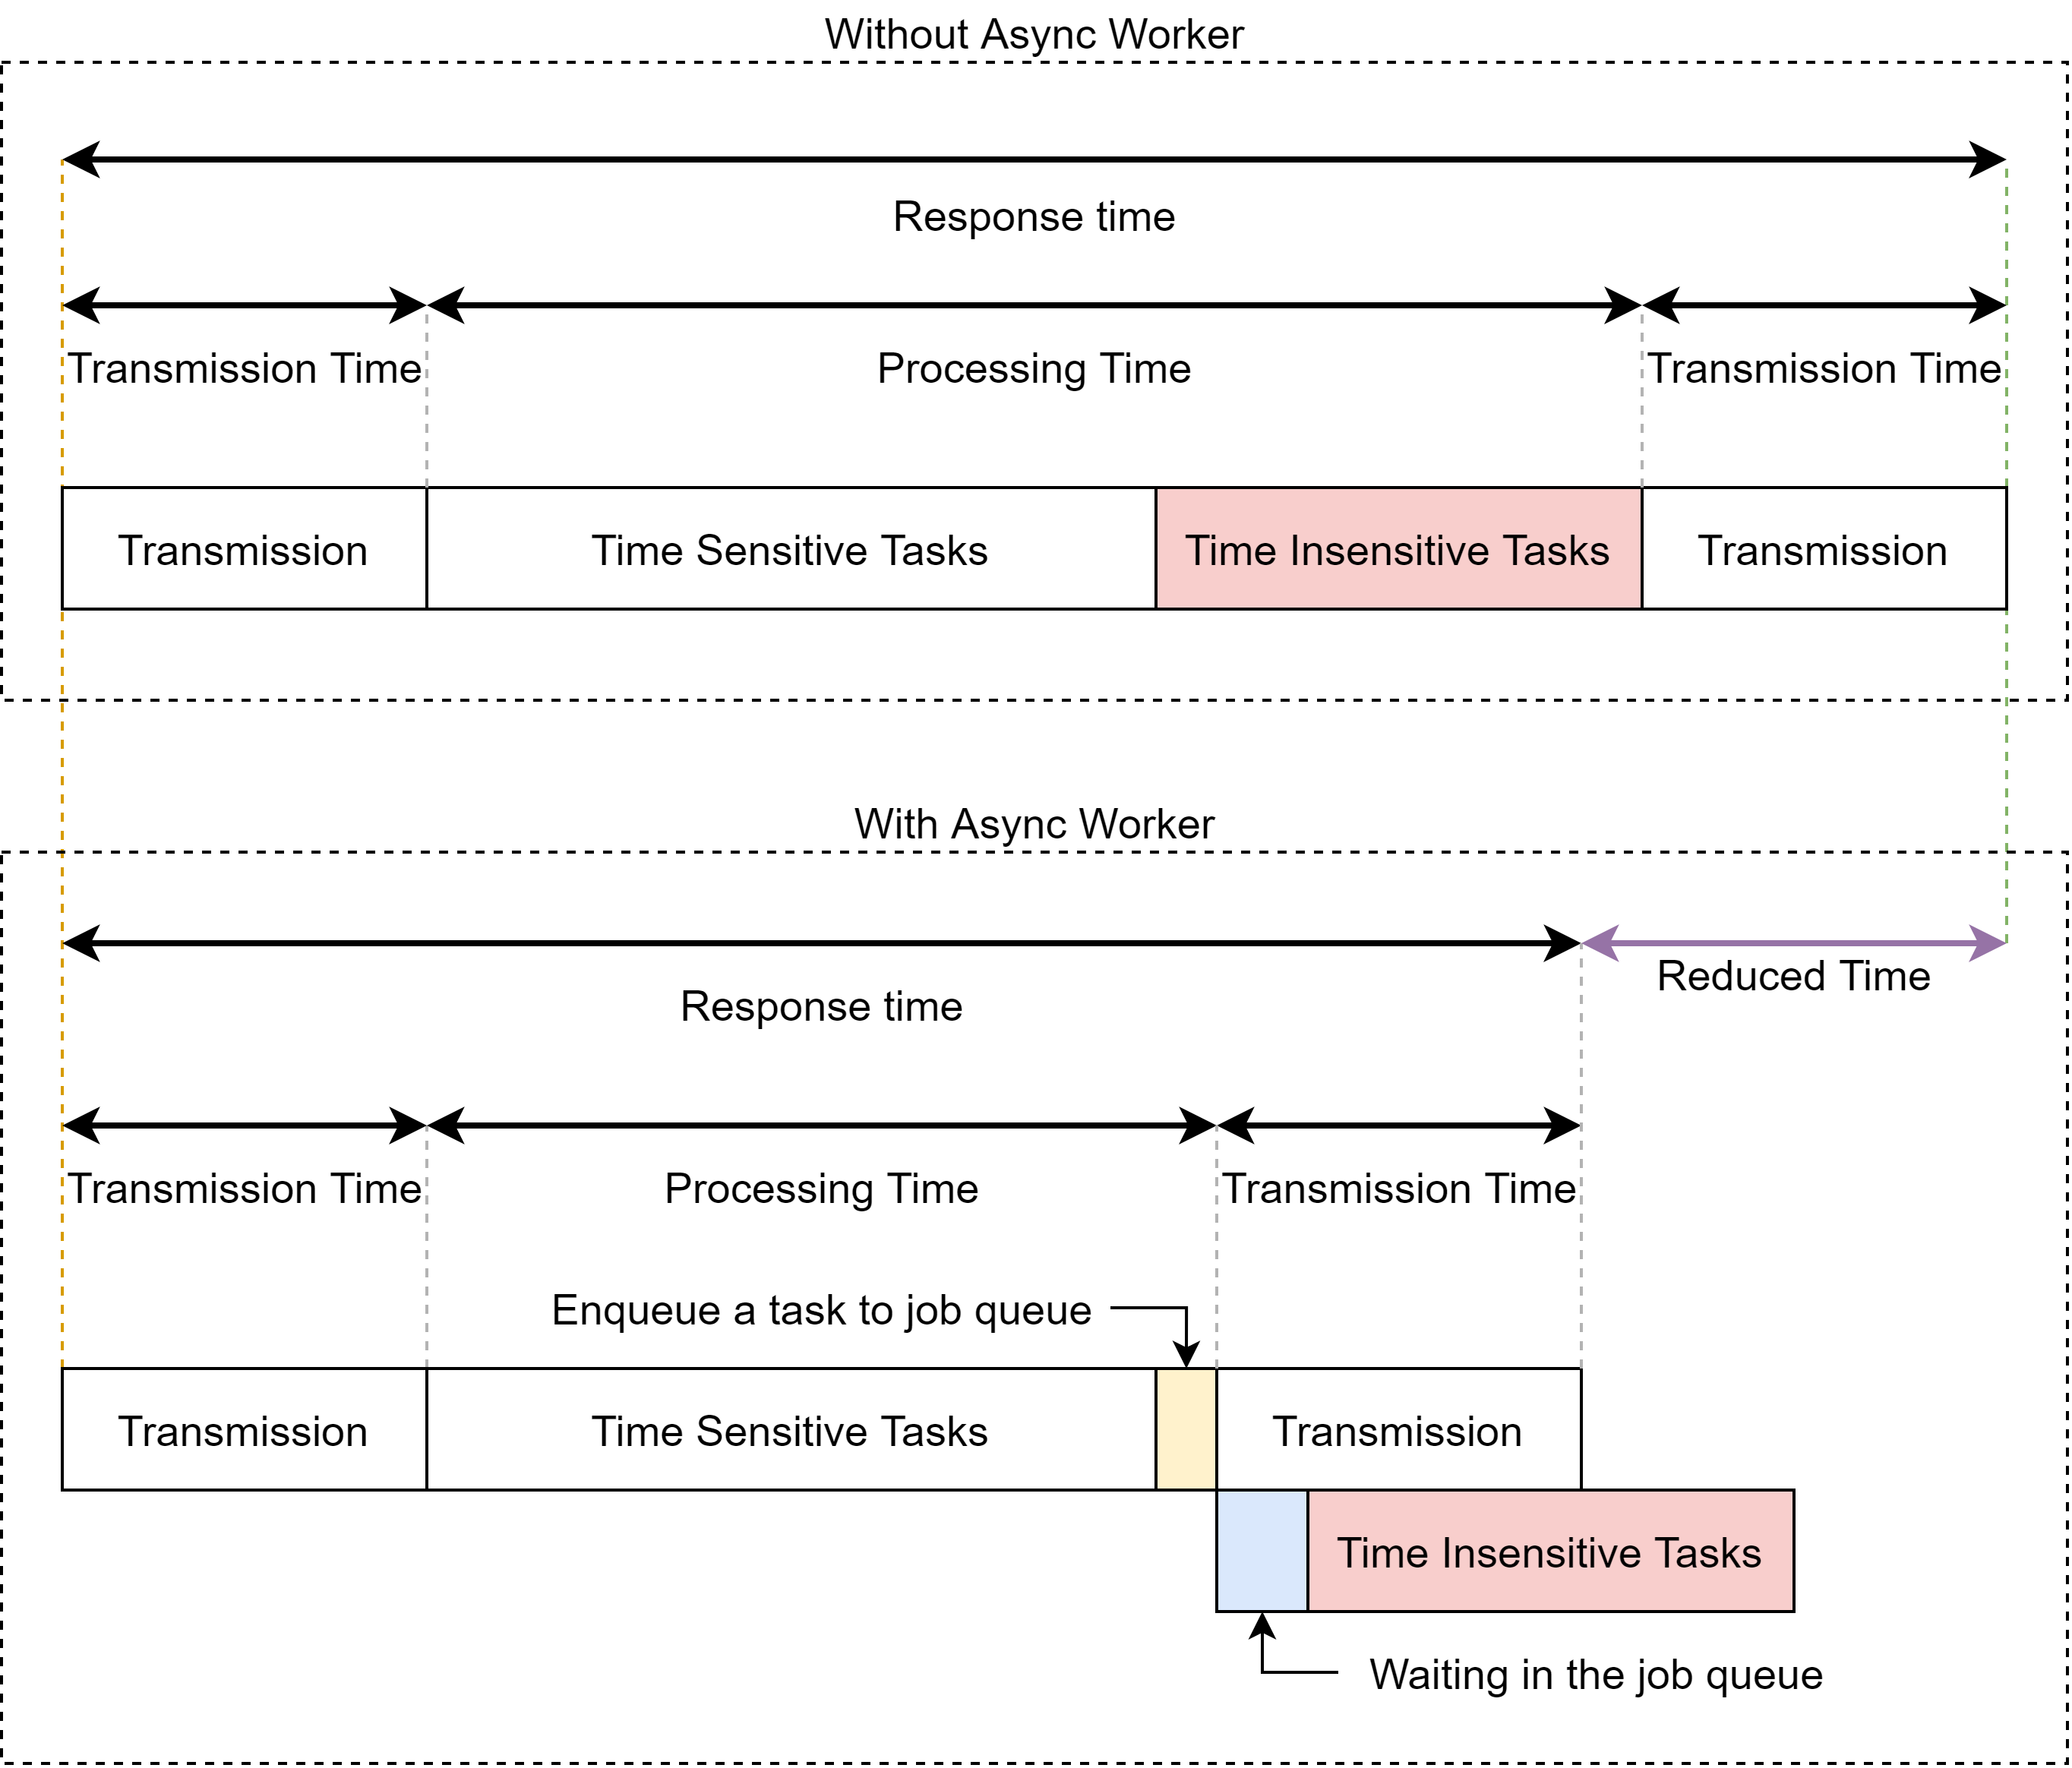
\includegraphics[width=\linewidth]{c4-asyncworker.png}
\caption{The comparison between using async worker and not.}
\label{fig:asyncworker}
\end{figure}

\begin{figure}[!ht]
\centering
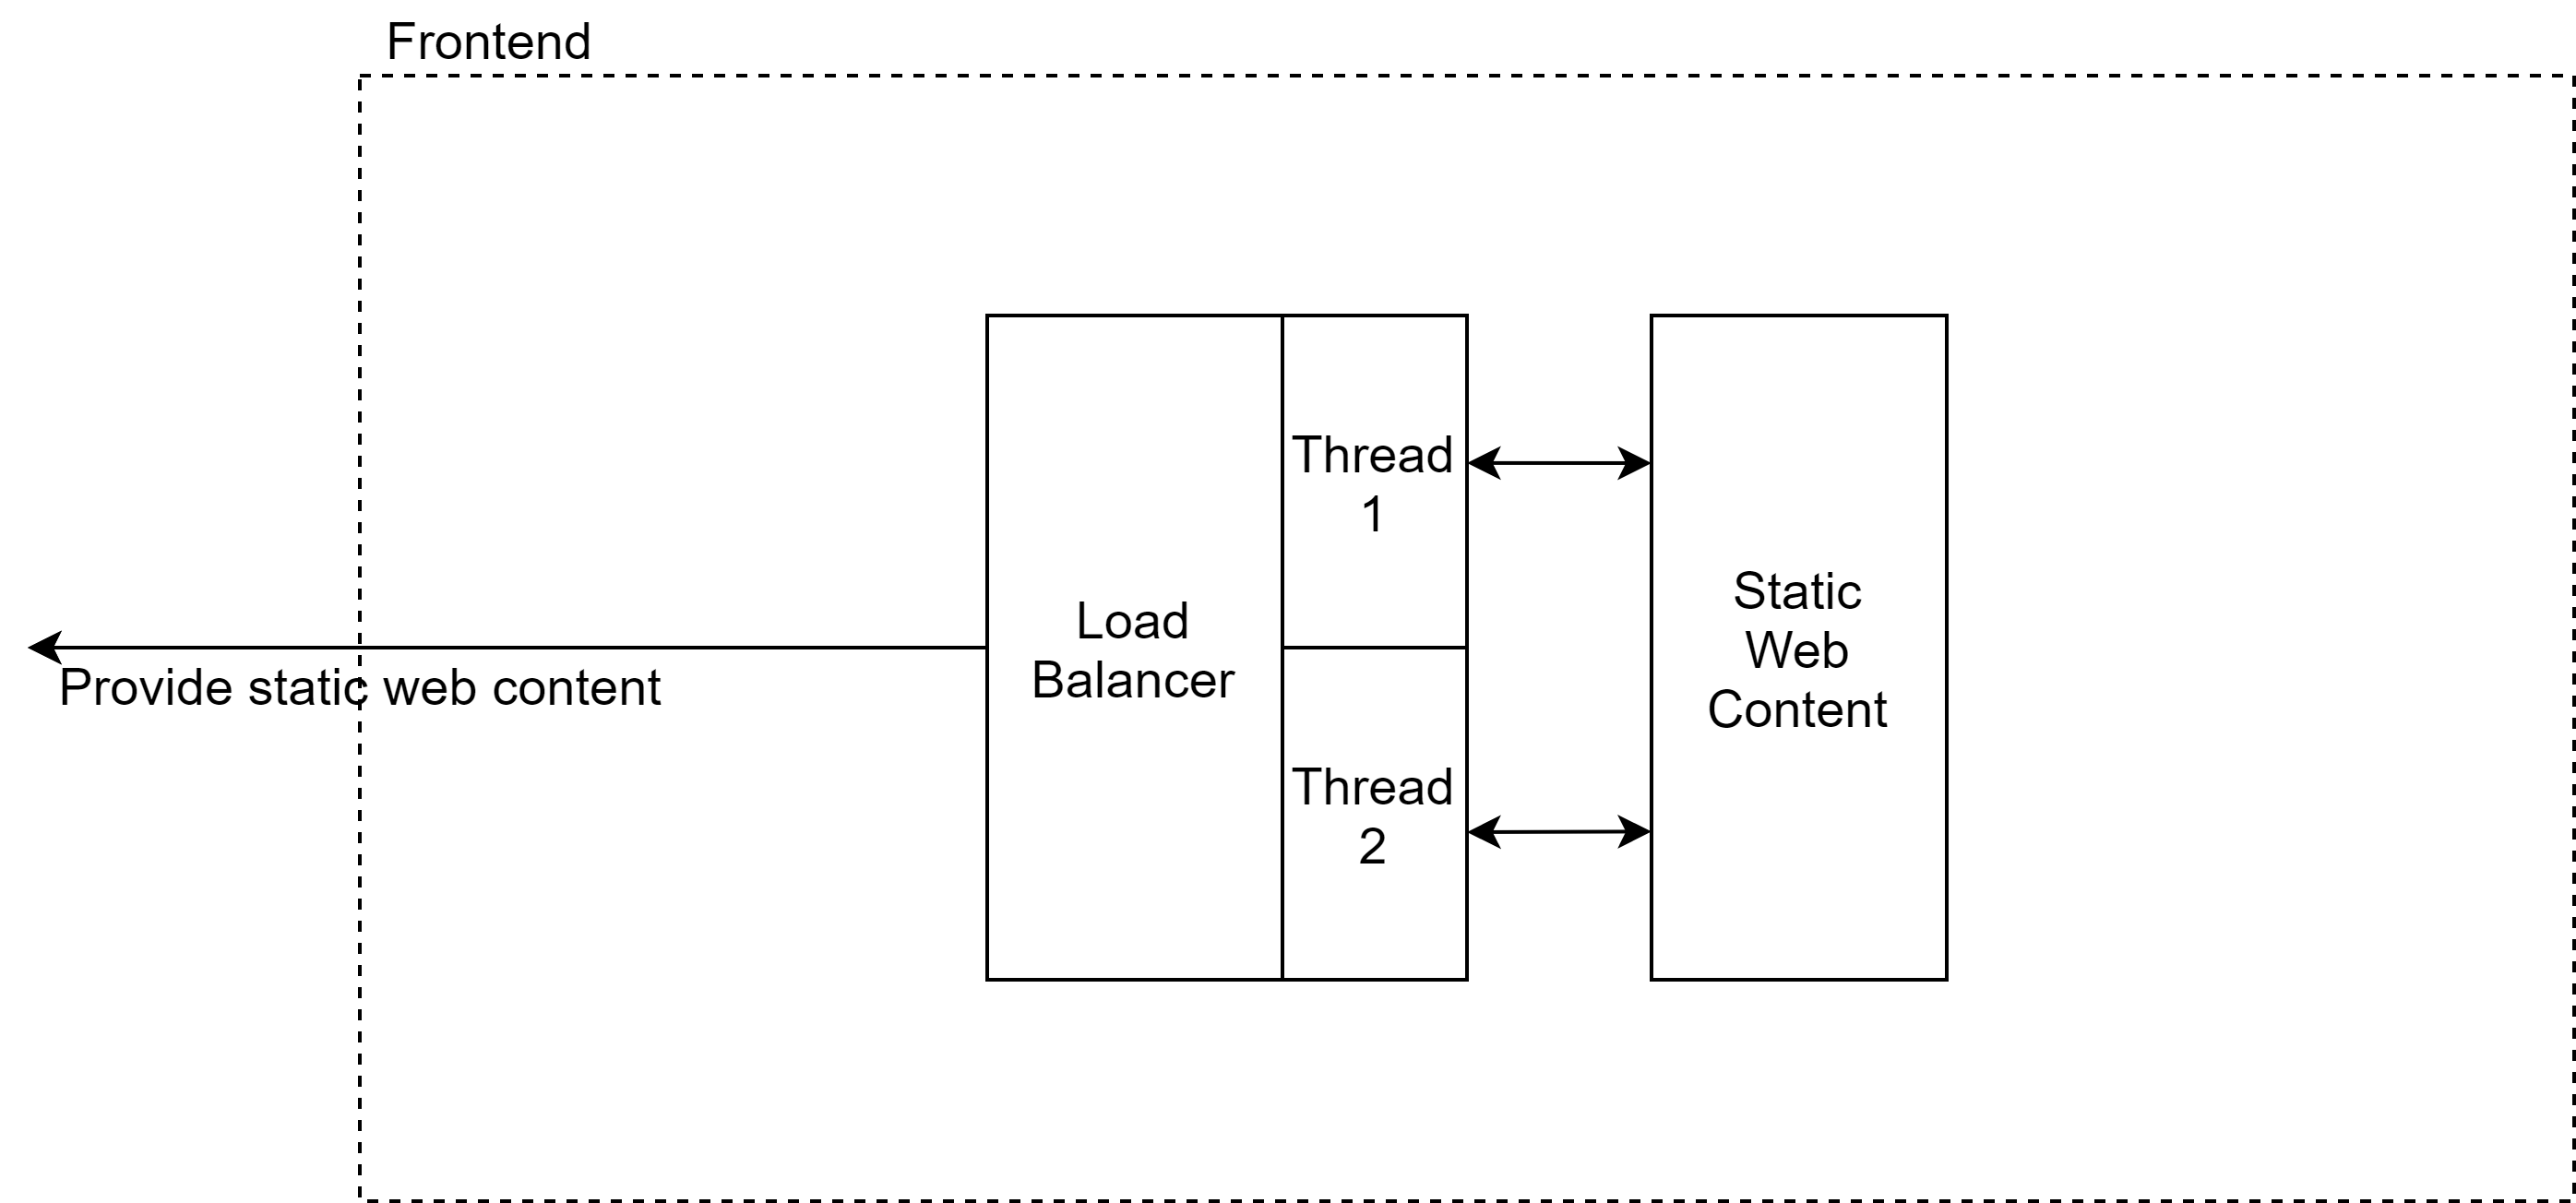
\includegraphics[width=\linewidth]{c4-frontend.png}
\caption{The architecture of the frontend composite component.}
\label{fig:frontend}
\end{figure}

\begin{figure}[!ht]
\centering
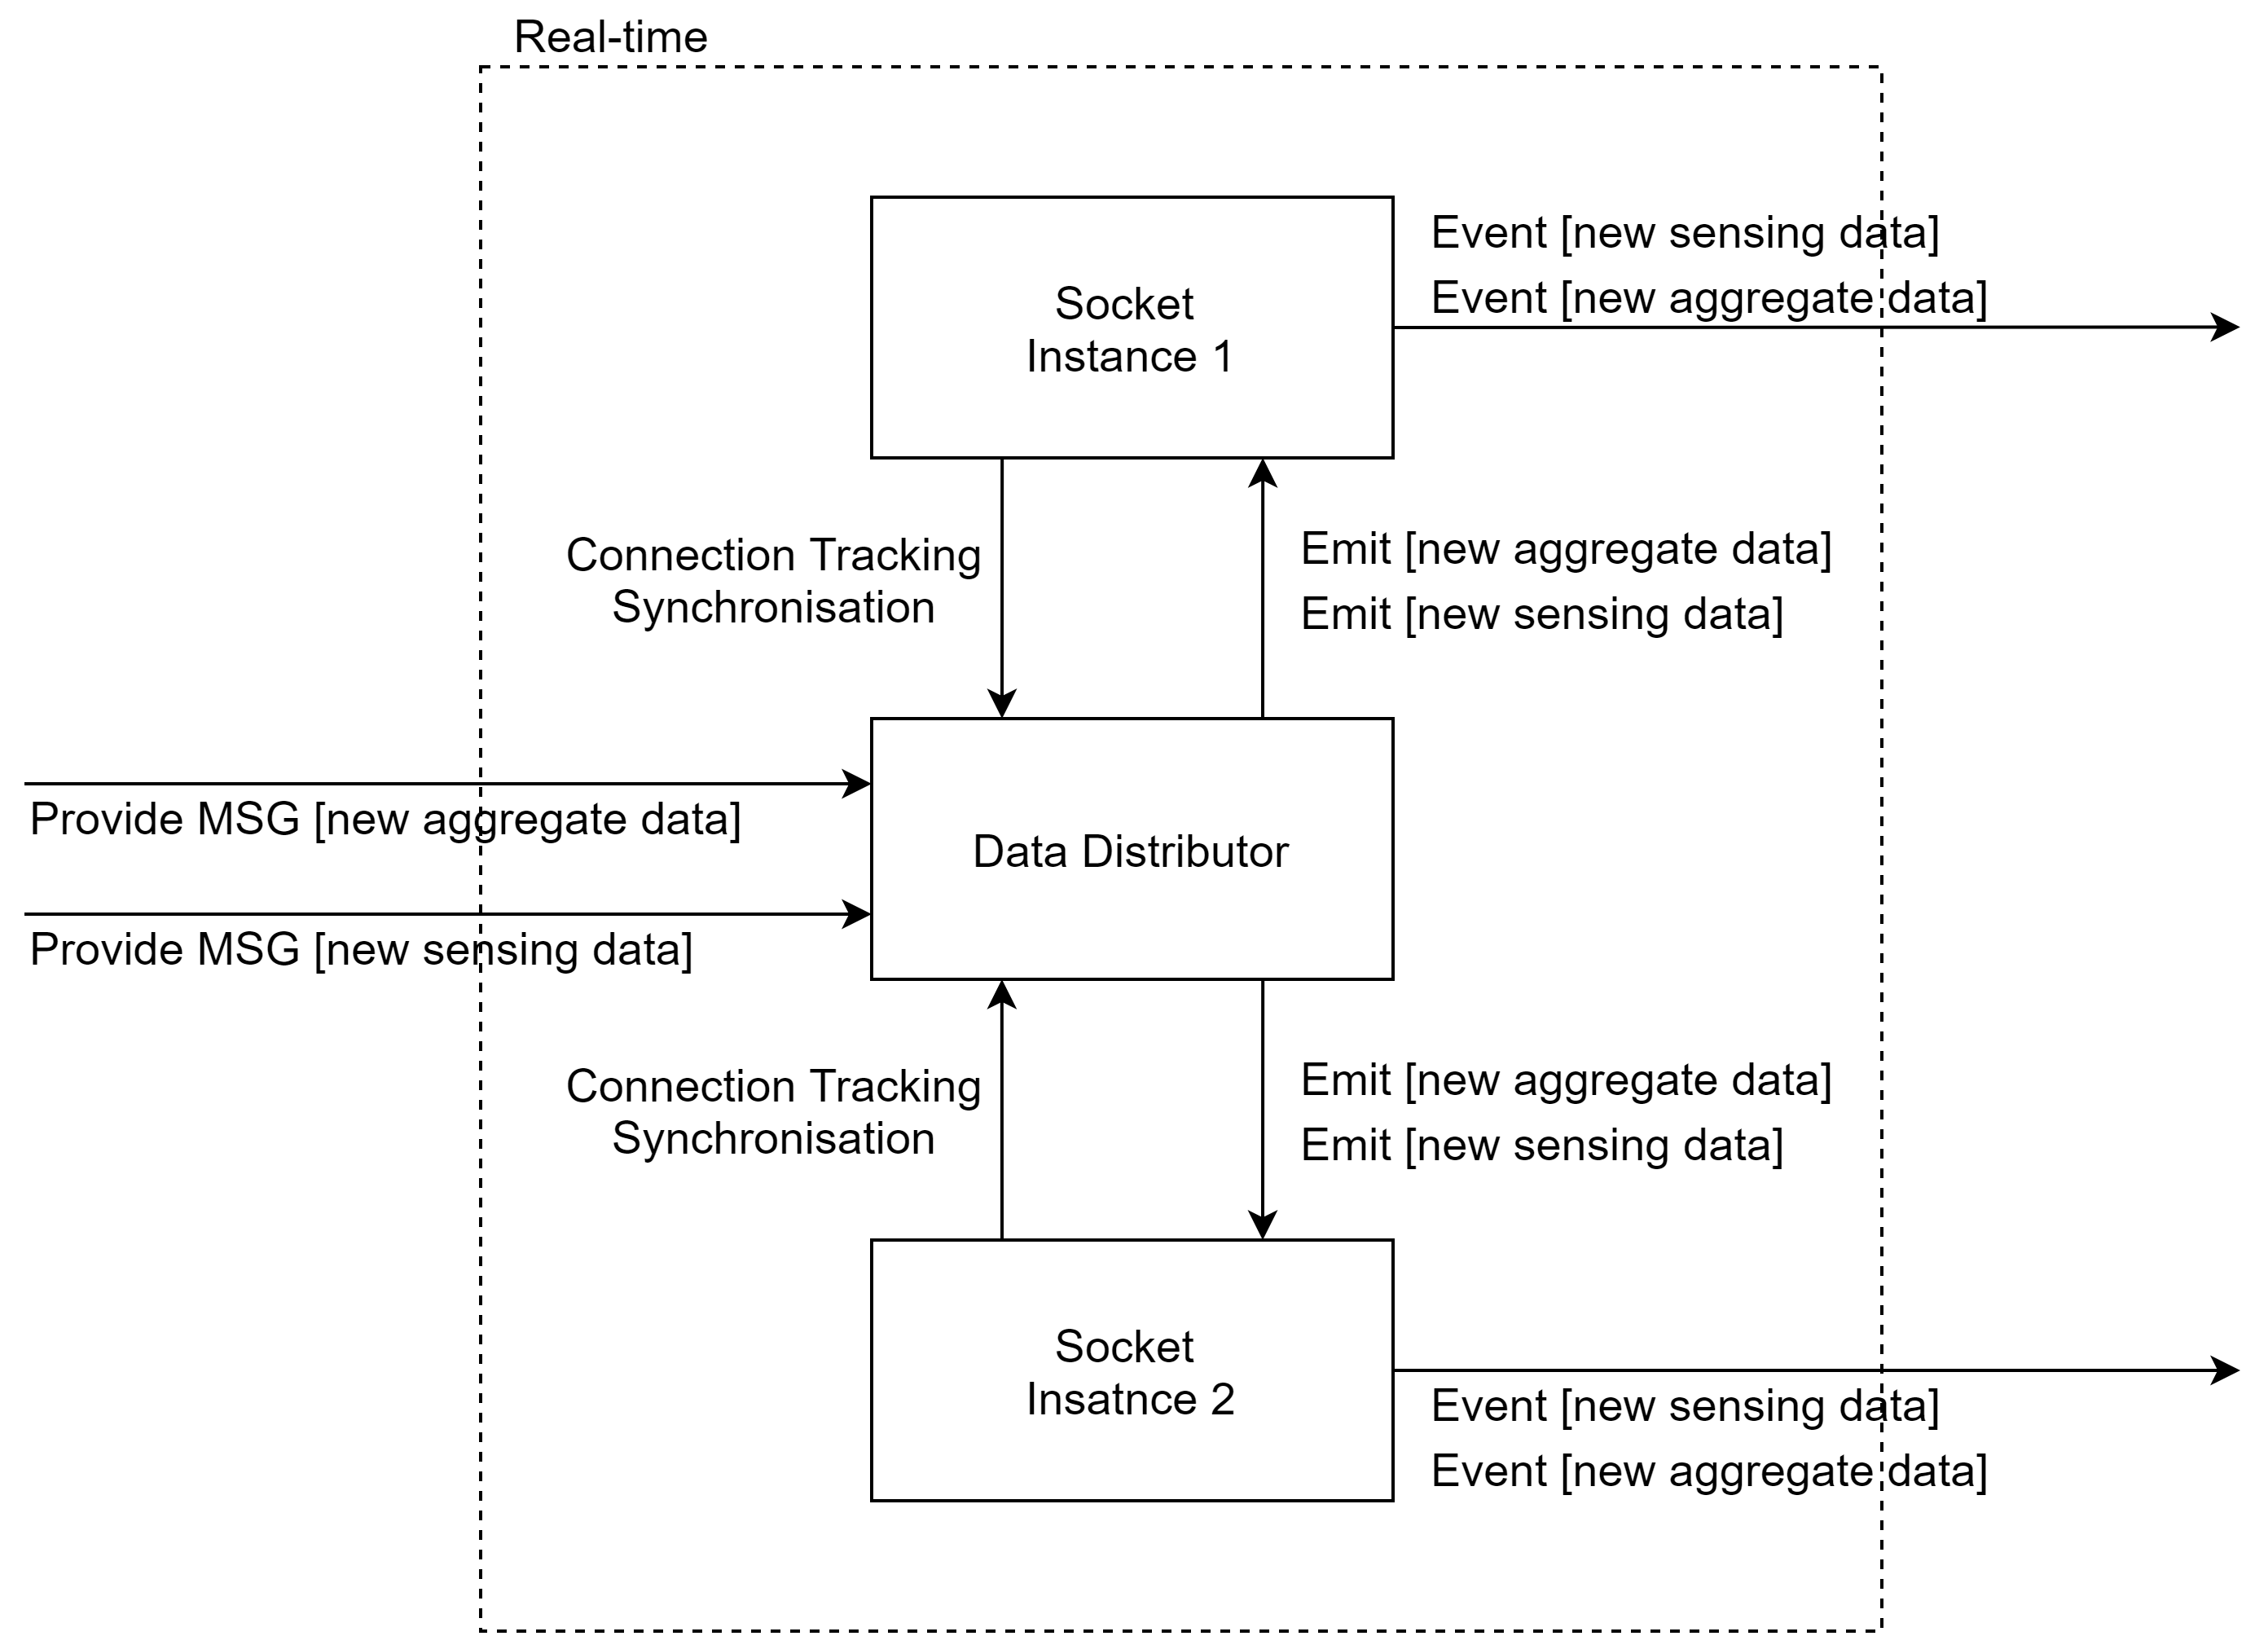
\includegraphics[width=\linewidth]{c4-realtime.png}
\caption{The architecture of the real-time composite component.}
\label{fig:realtime}
\end{figure}

\begin{figure}[!ht]
\centering
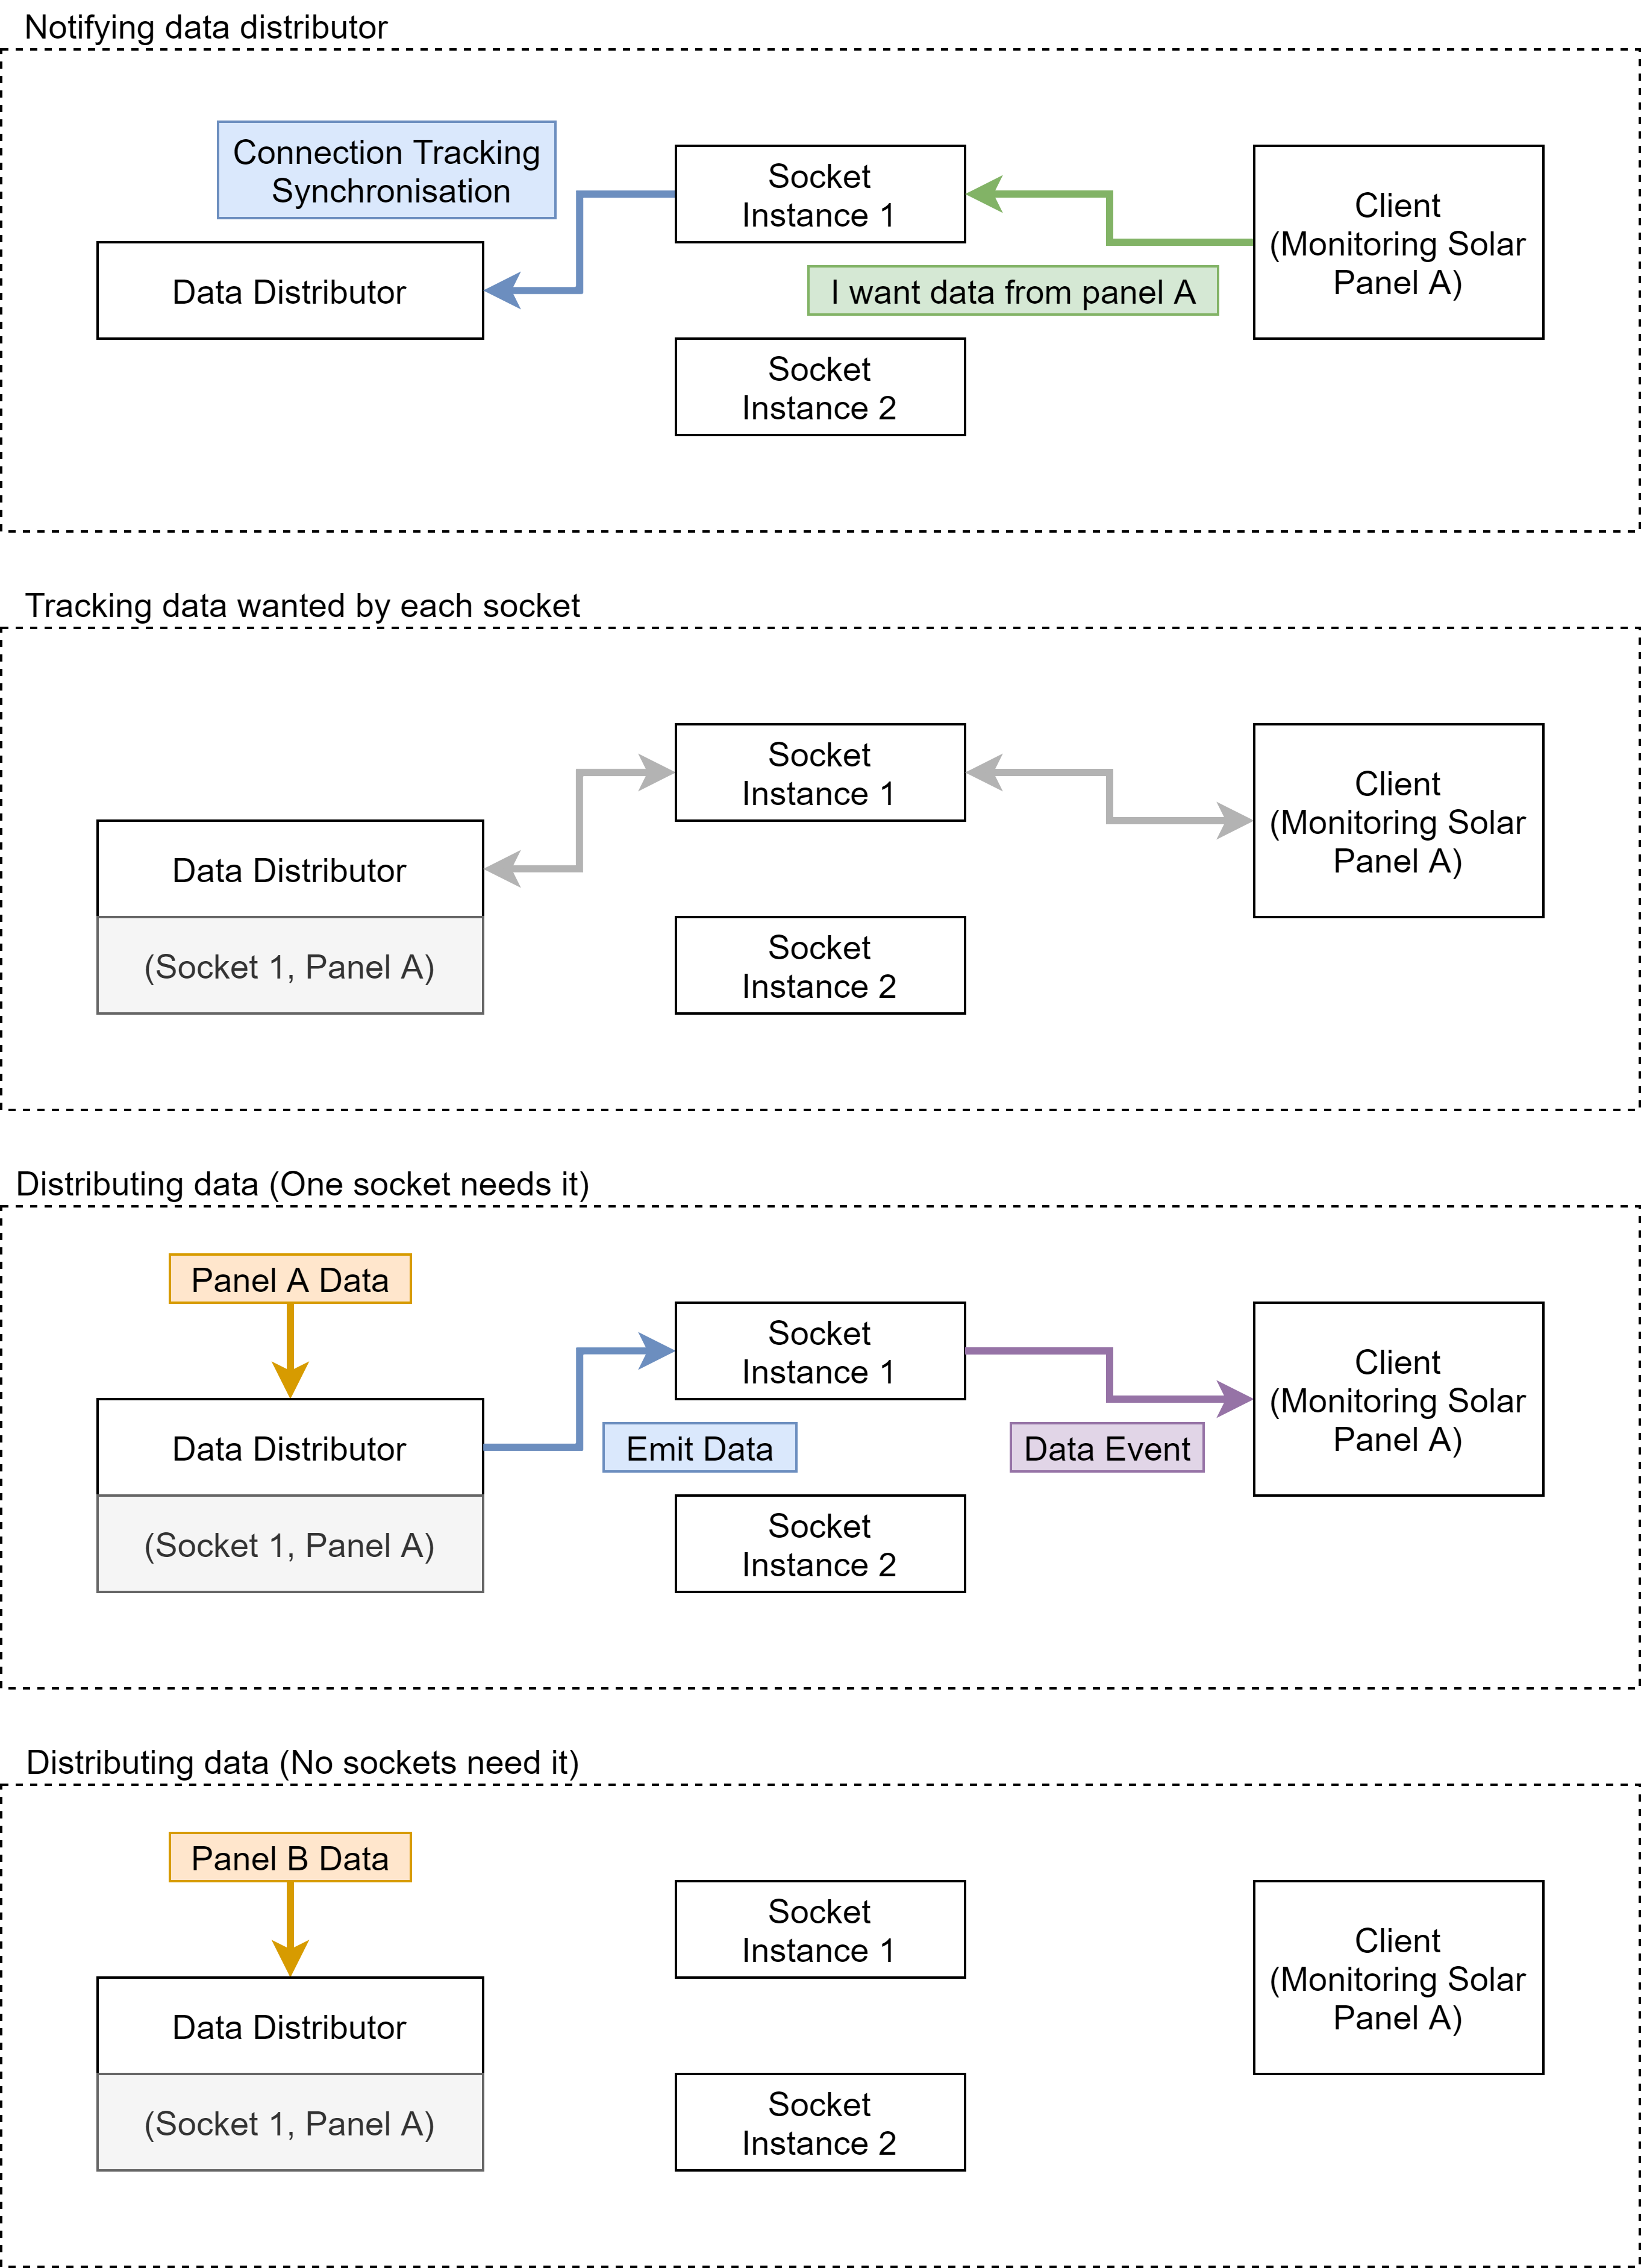
\includegraphics[width=\linewidth]{c4-rtscenario1.png}
\caption{The data distributor innerworkings after clients connected.}
\label{fig:rtscenario1}
\end{figure}

\begin{figure}[!ht]
\centering
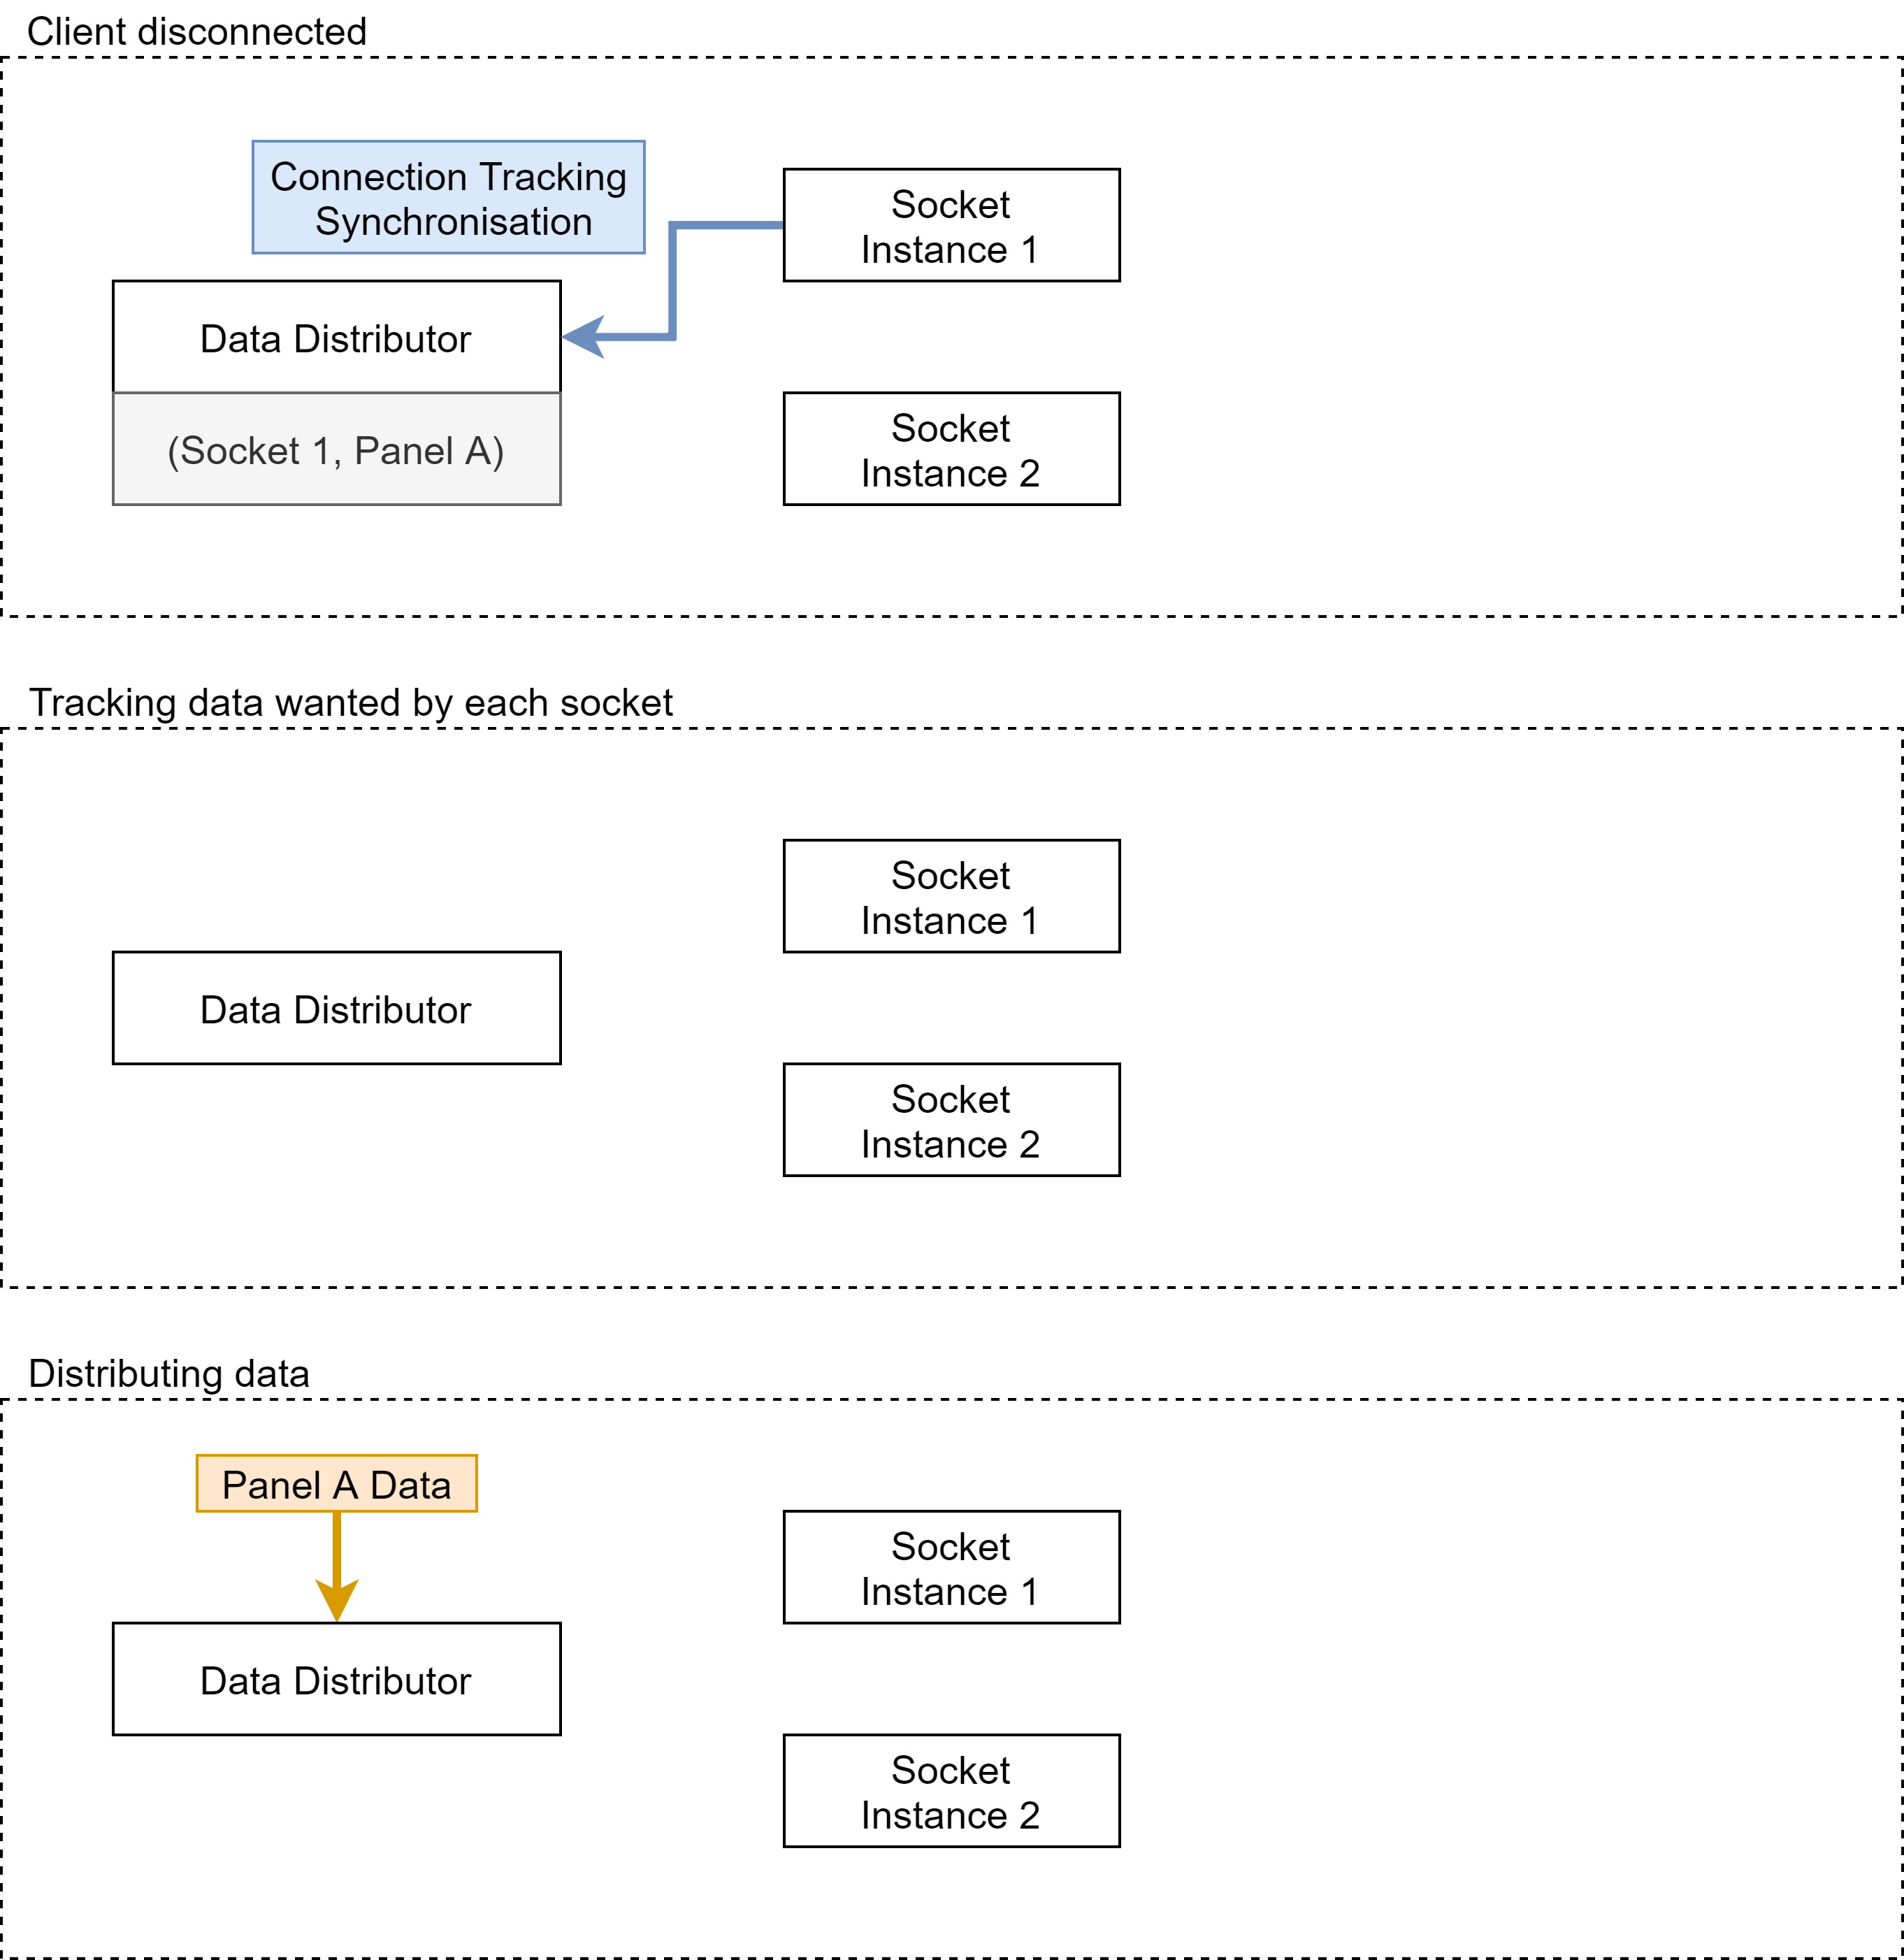
\includegraphics[width=\linewidth]{c4-rtscenario2.png}
\caption{The data distributor innerworkings after clients disconnected.}
\label{fig:rtscenario2}
\end{figure}

\begin{figure}[!ht]
\centering
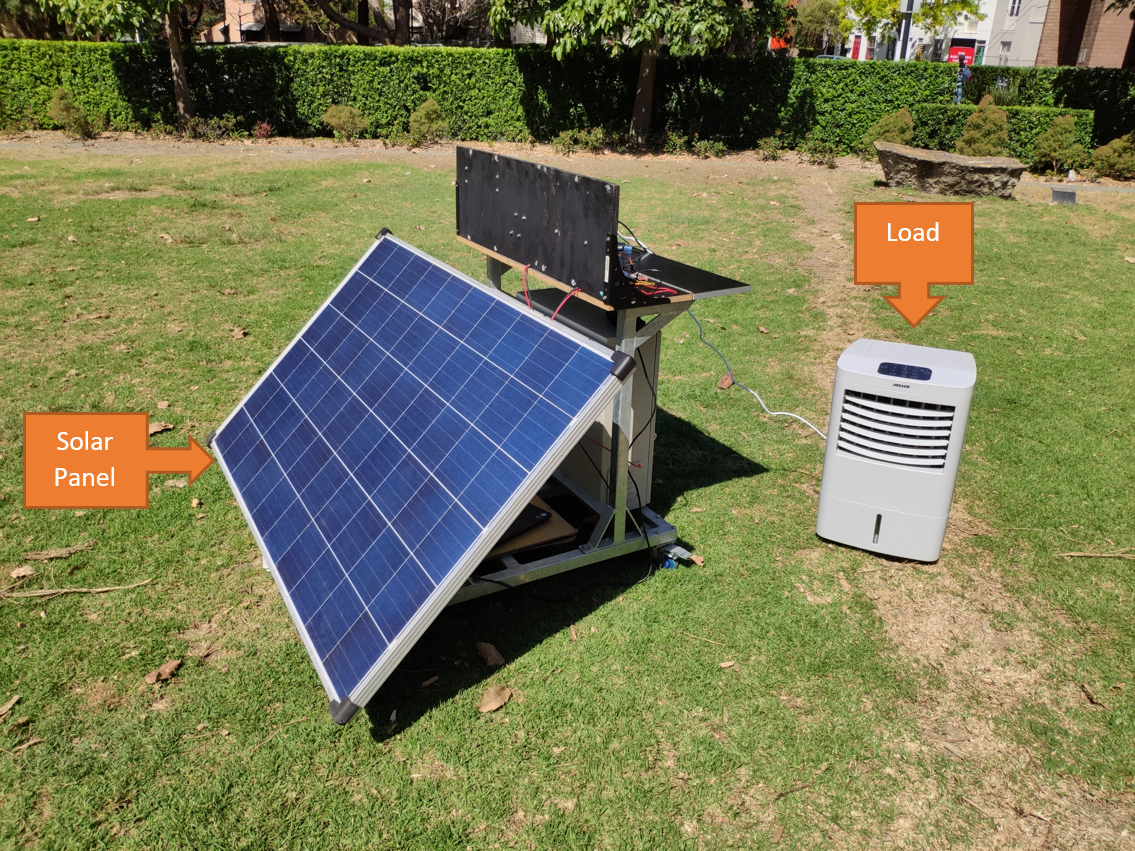
\includegraphics[width=0.8\linewidth]{realworld1.png}
\caption{The experimental setup (front)}
\label{fig:realworld1}
\end{figure}

\begin{figure}[!ht]
\centering
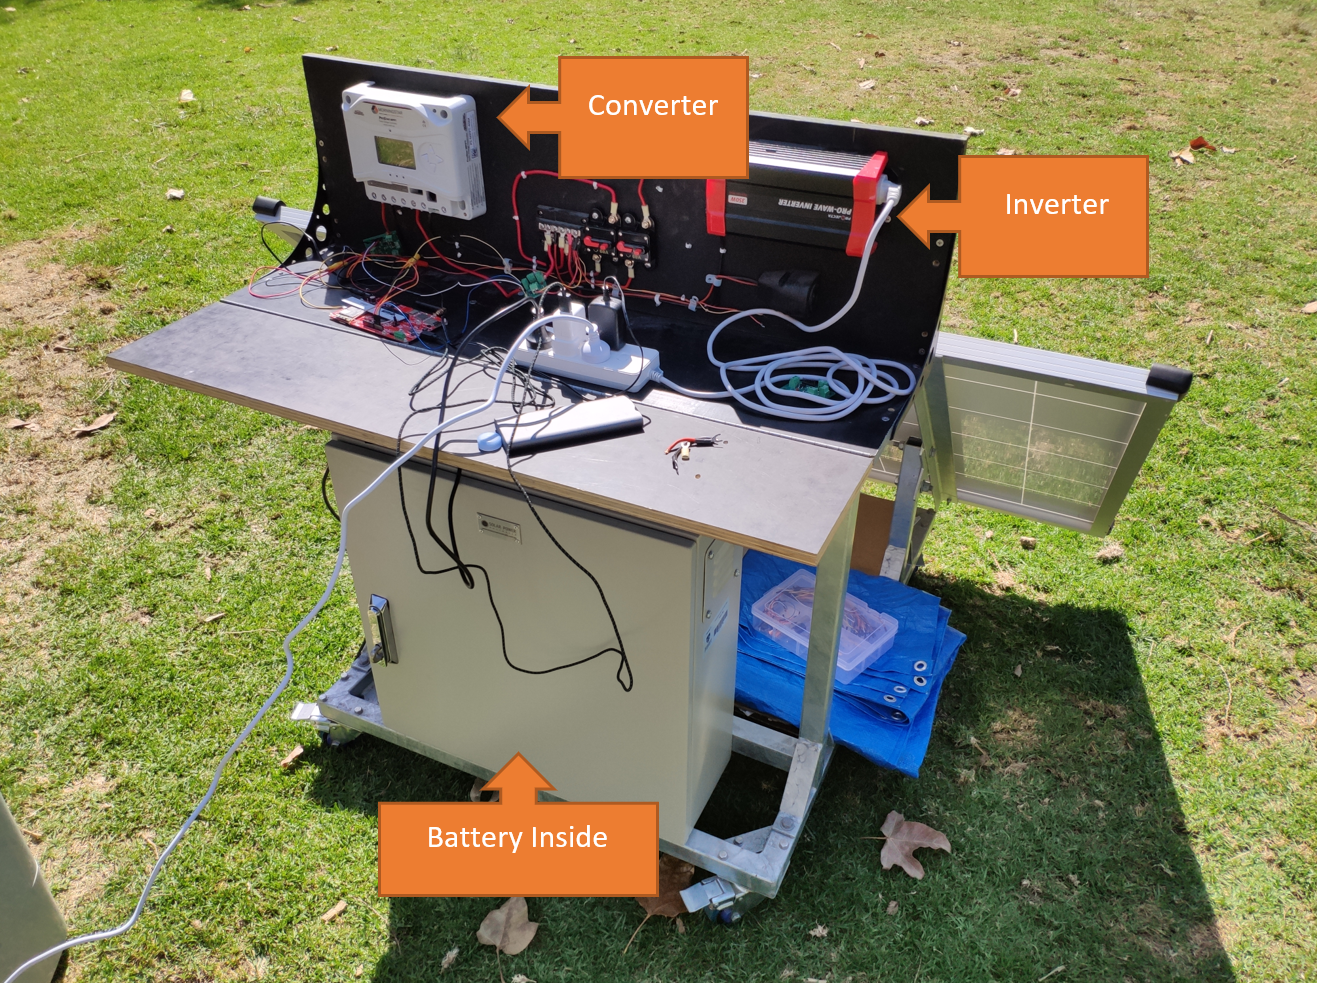
\includegraphics[width=0.8\linewidth]{realworld2.png}
\caption{The experimental setup (back)}
\label{fig:realworld2}
\end{figure}

\begin{figure}[!ht]
\centering
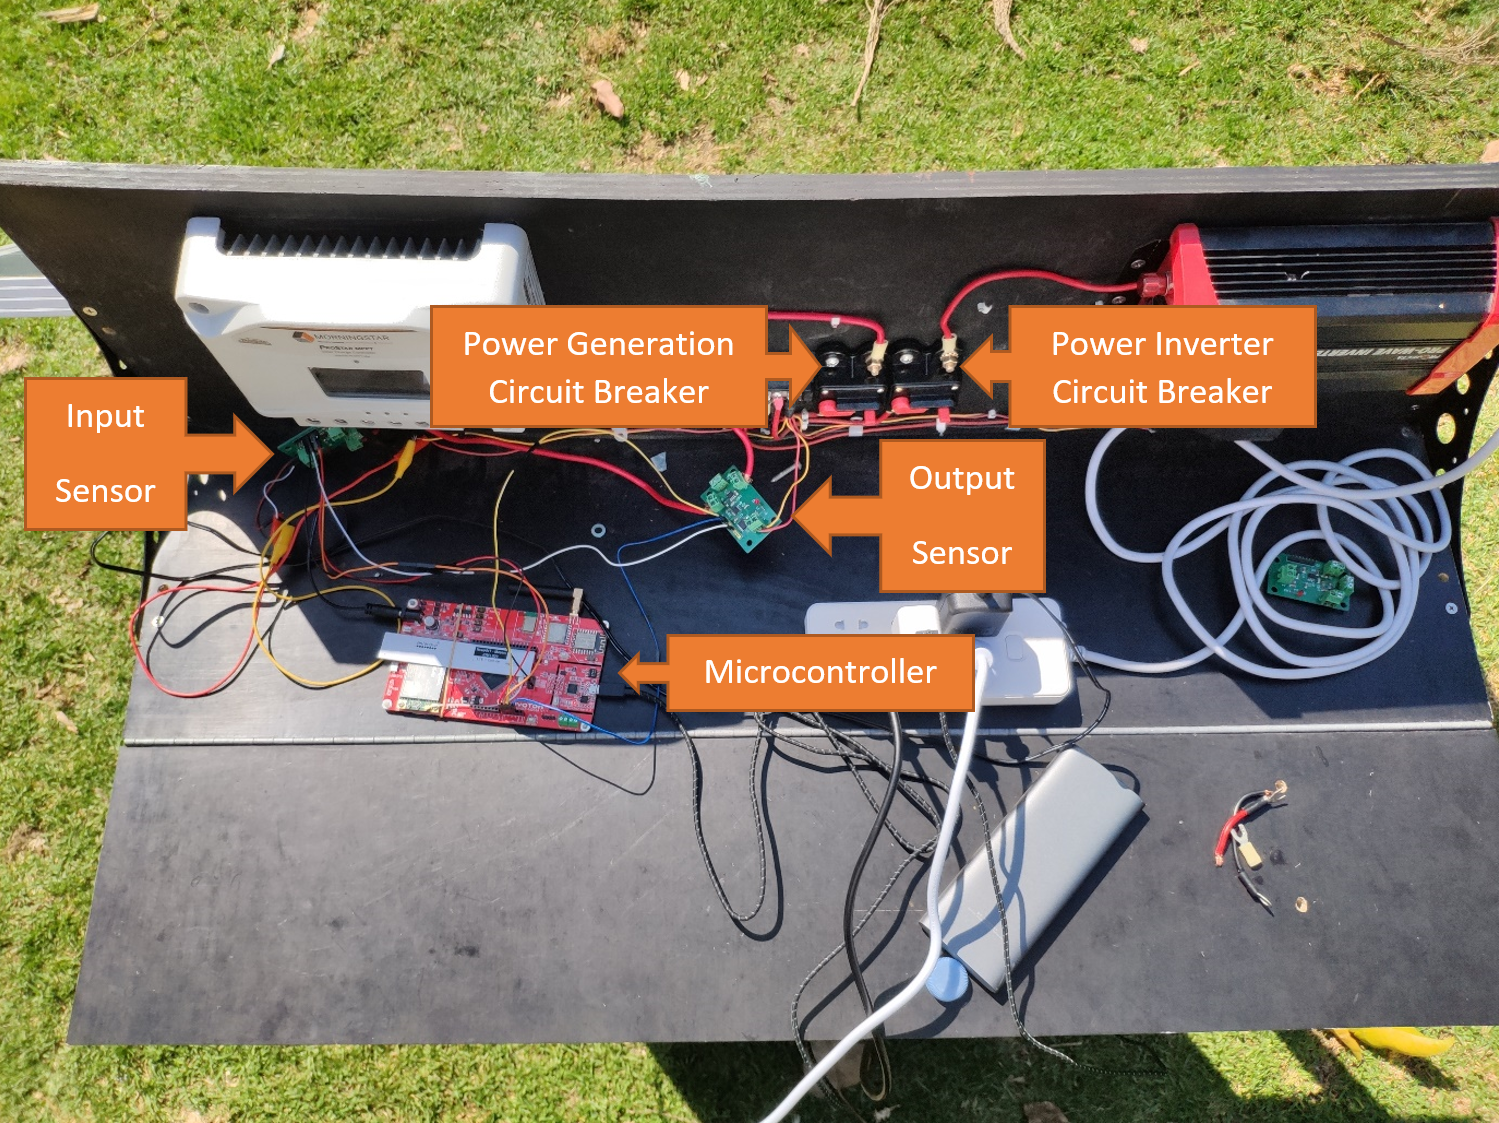
\includegraphics[width=0.8\linewidth]{realworld3.png}
\caption{The experimental setup (top)}
\label{fig:realworld3}
\end{figure}

\begin{figure}[!ht]
\centering
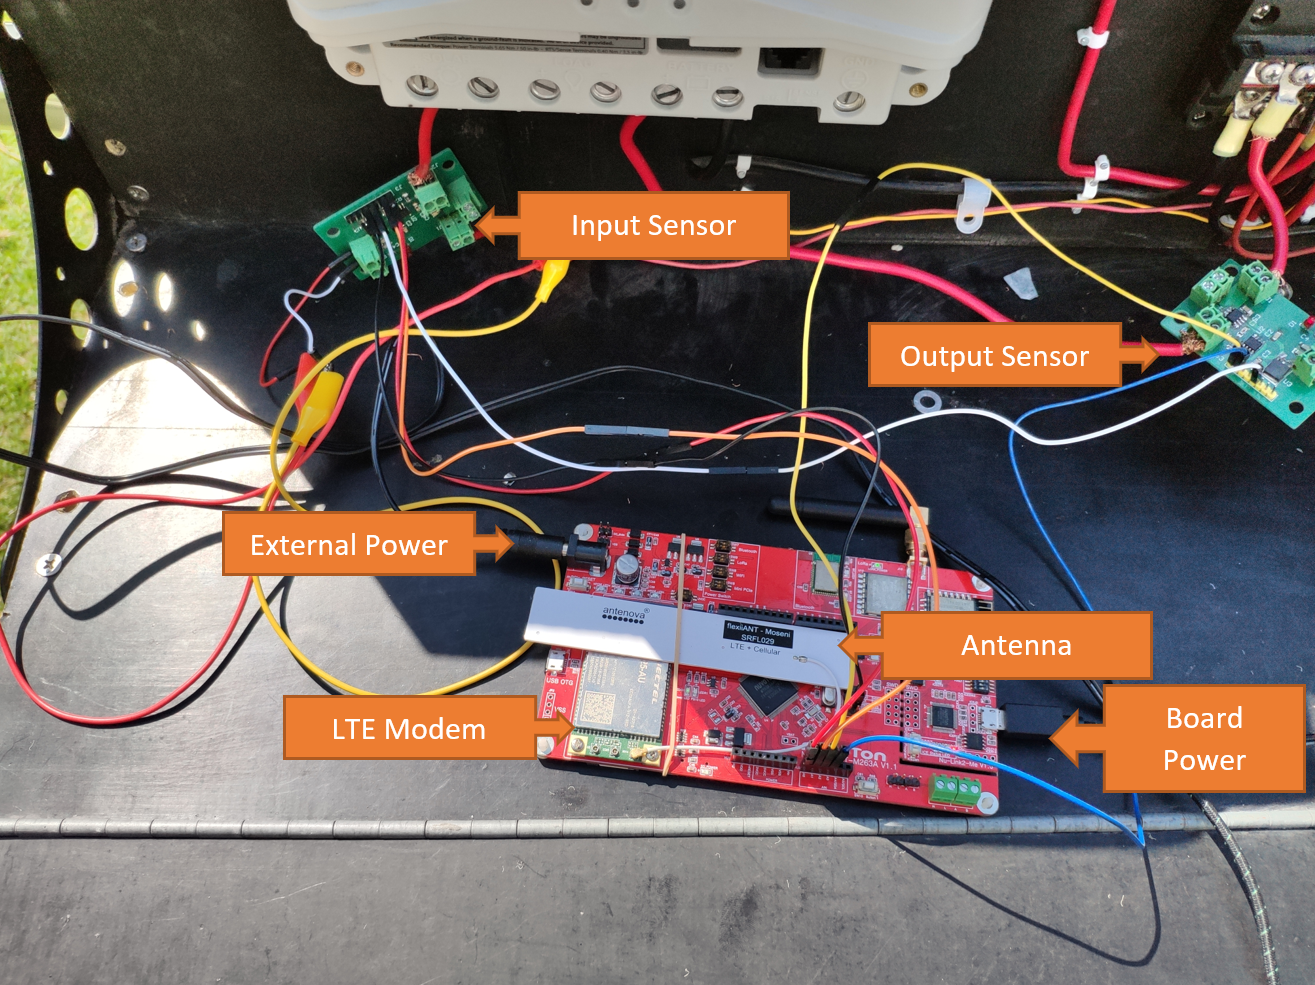
\includegraphics[width=0.8\linewidth]{realworld4.png}
\caption{The experimental setup (controller)}
\label{fig:realworld4}
\end{figure}

\begin{figure}[!ht]
\centering
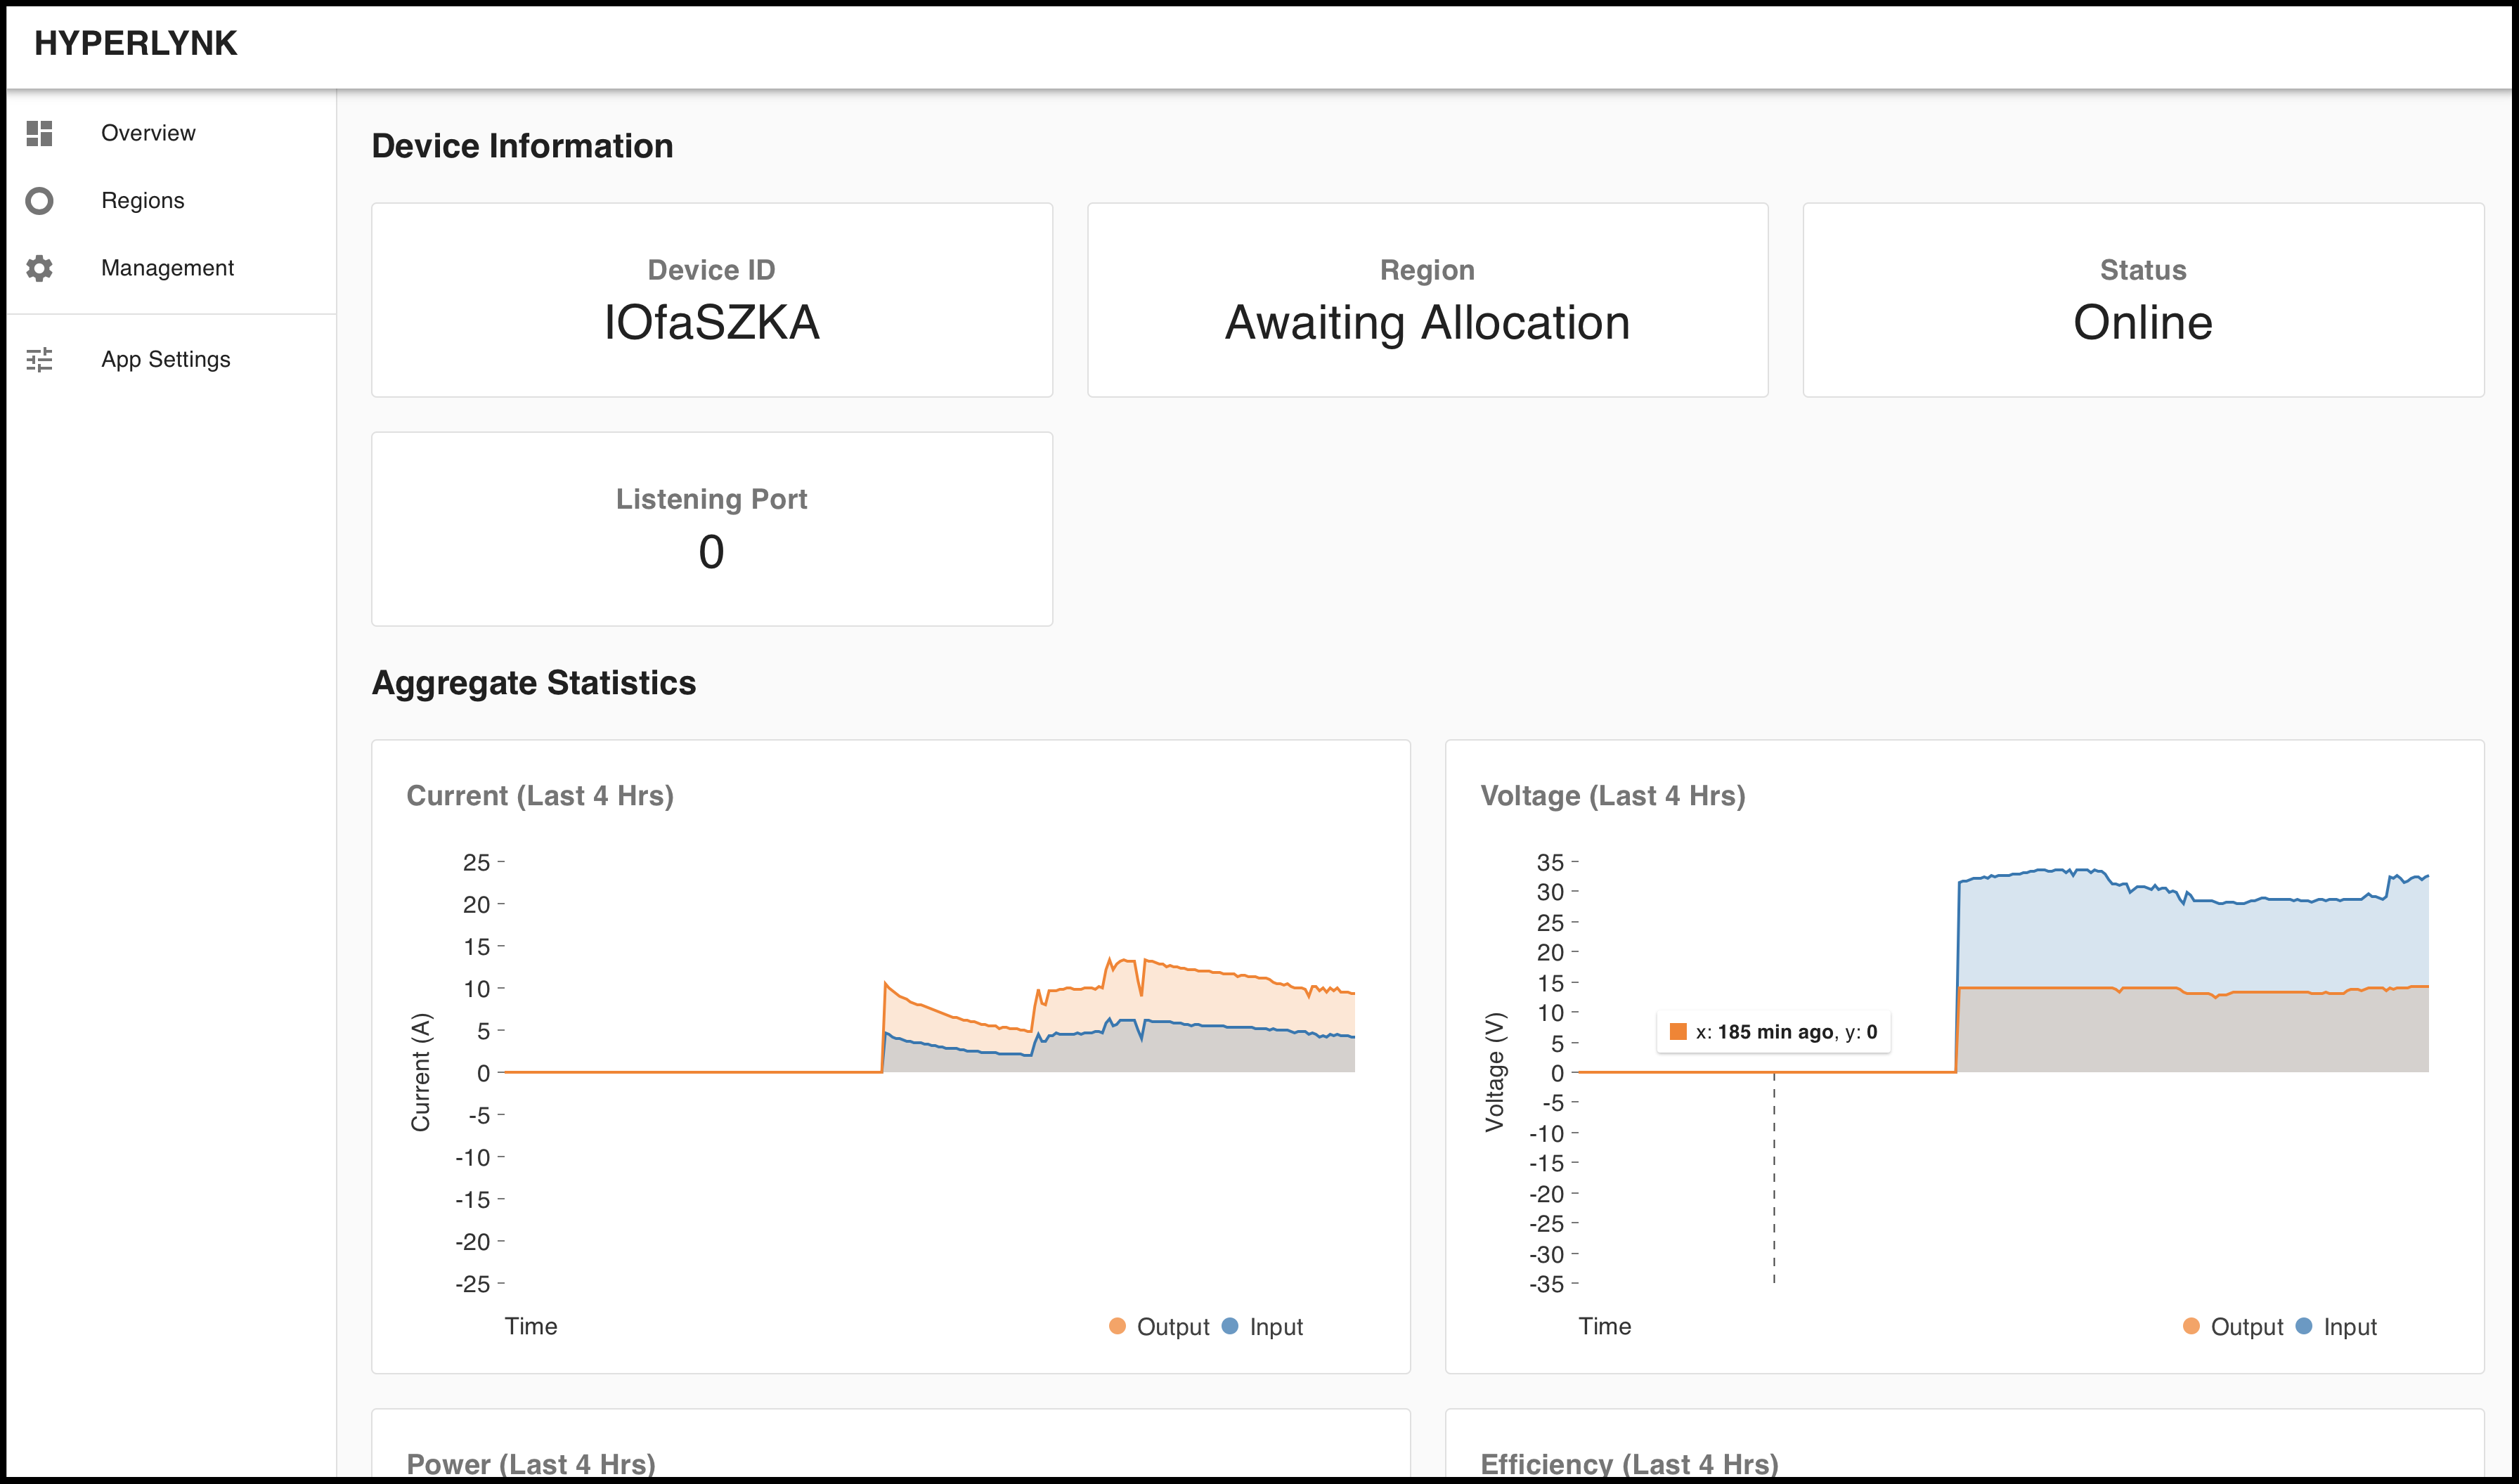
\includegraphics[width=\linewidth]{page1.png}
\caption{The website showing the device information.}
\label{fig:page1}
\end{figure}

\begin{figure}[!ht]
\centering
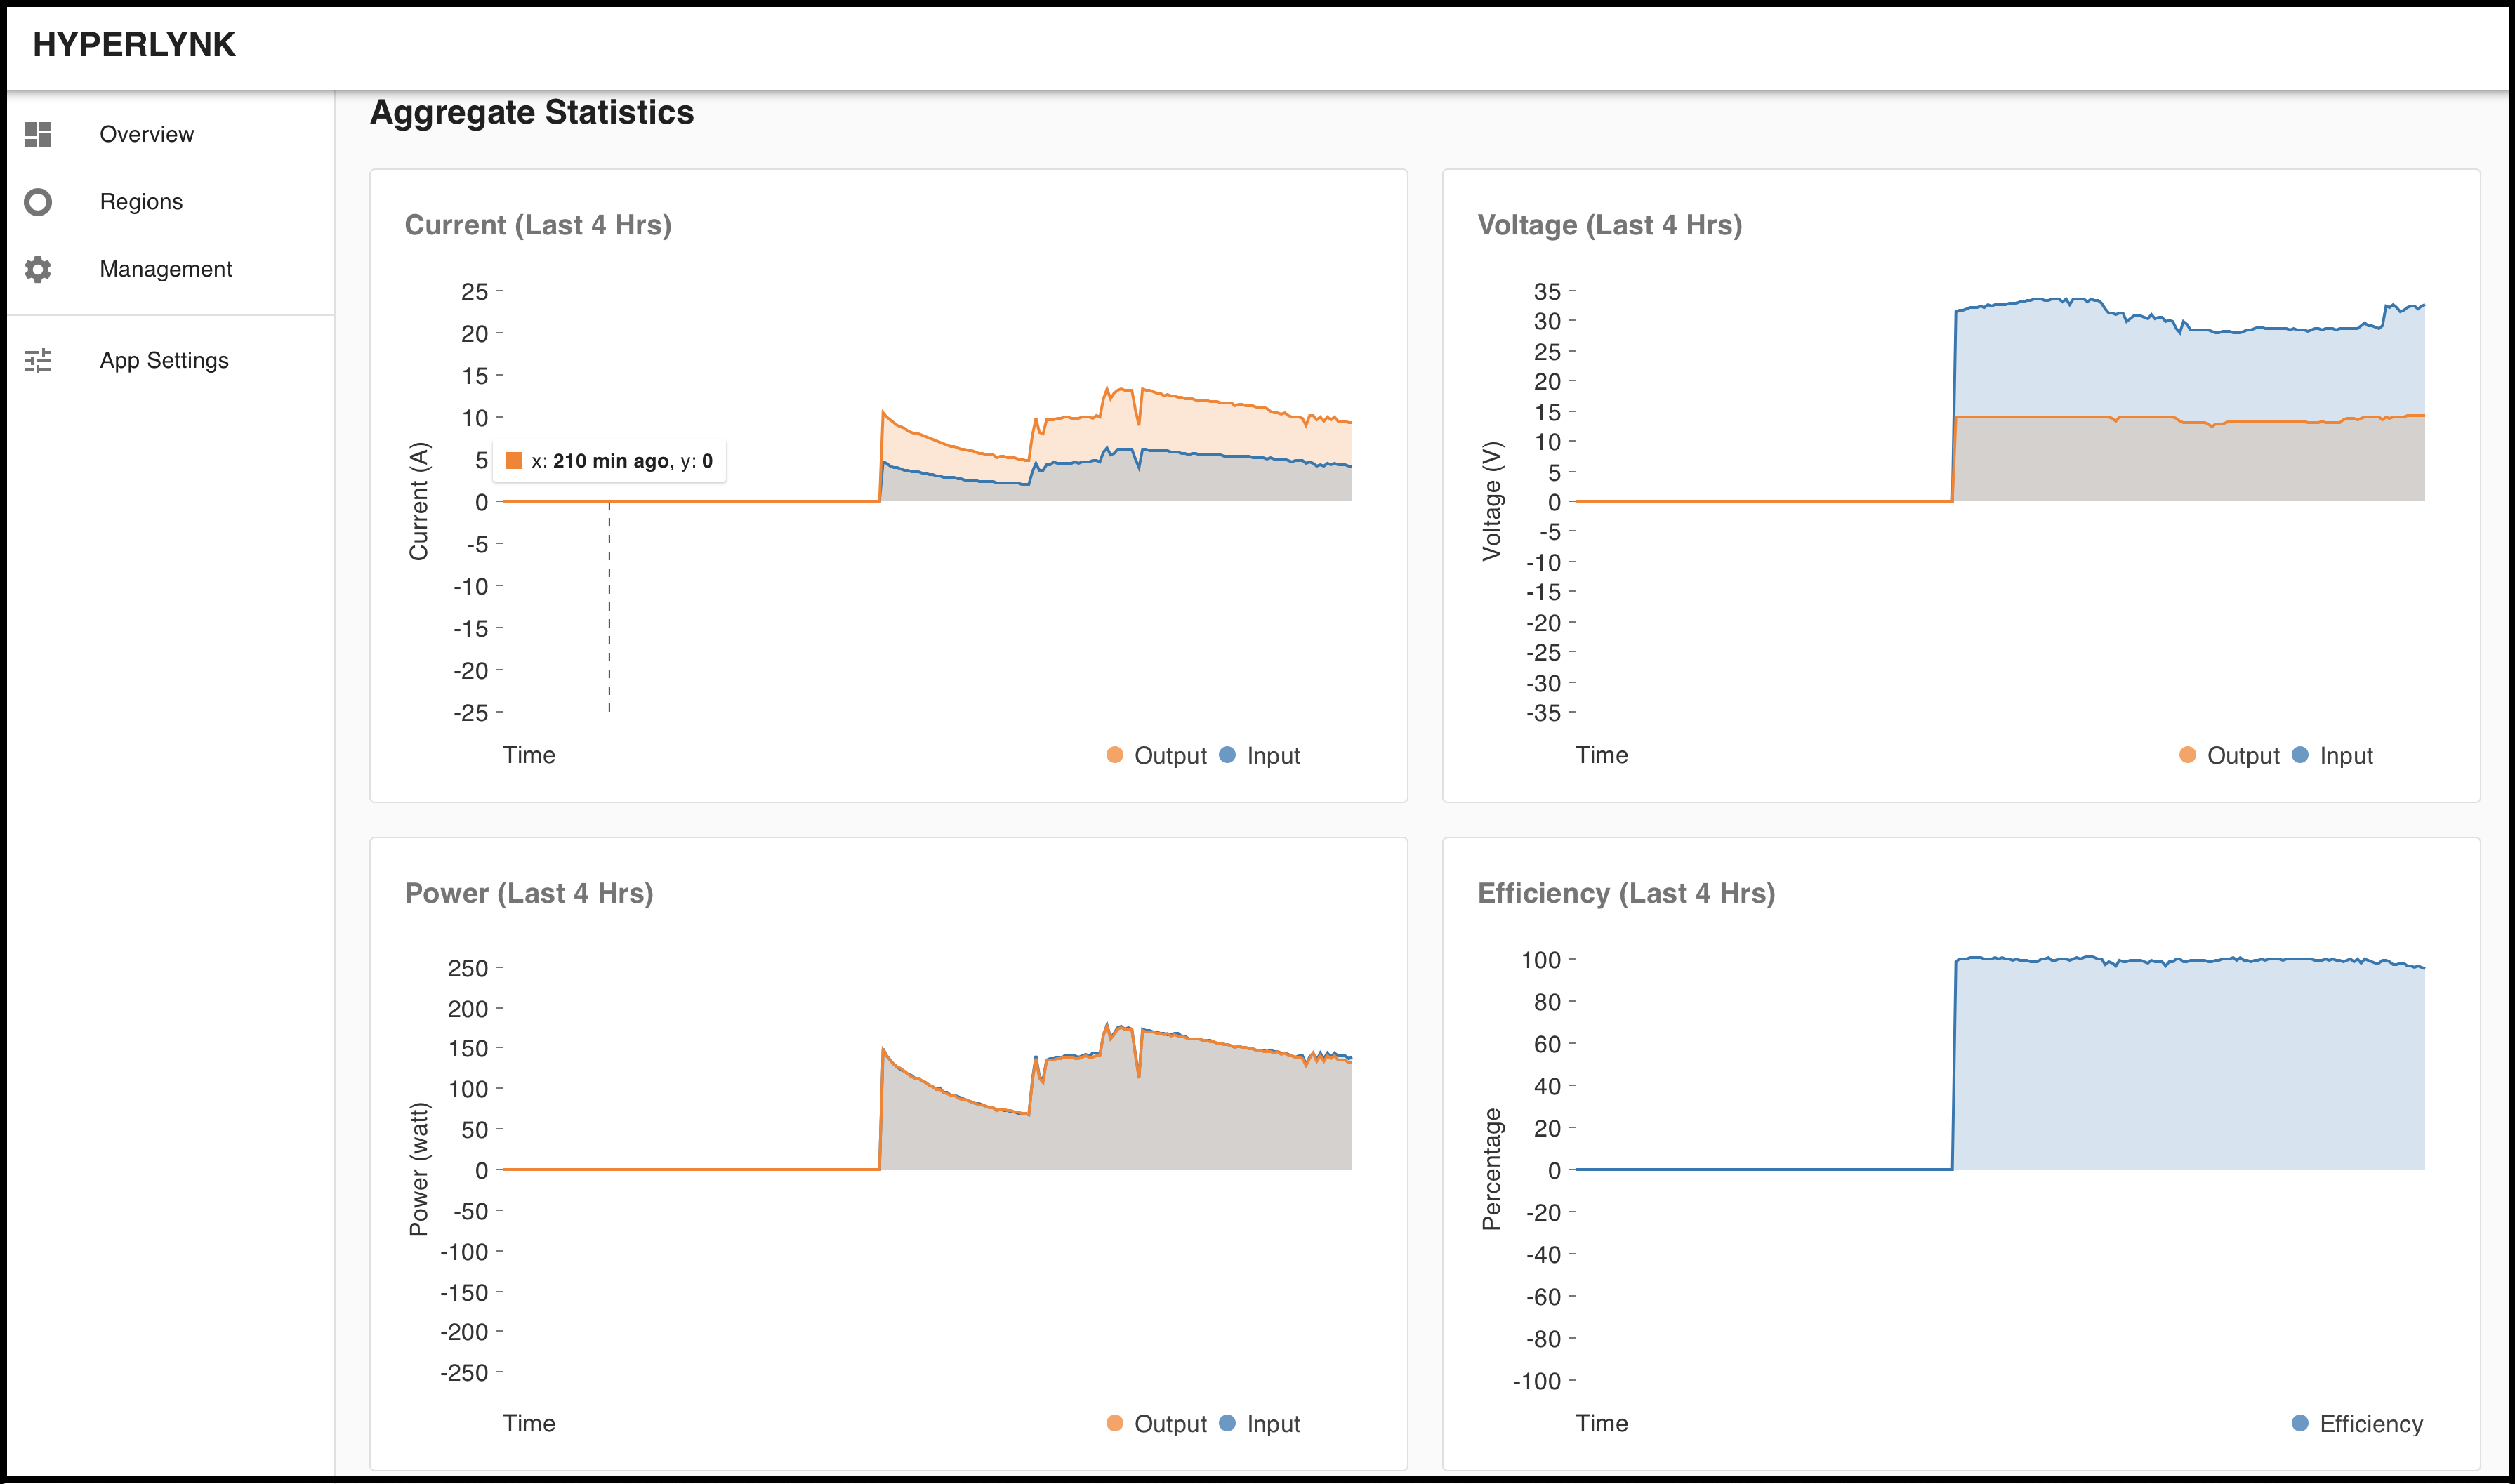
\includegraphics[width=\linewidth]{page2.png}
\caption{The website showing the aggregate data.}
\label{fig:page2}
\end{figure}

\begin{figure}[!ht]
\centering
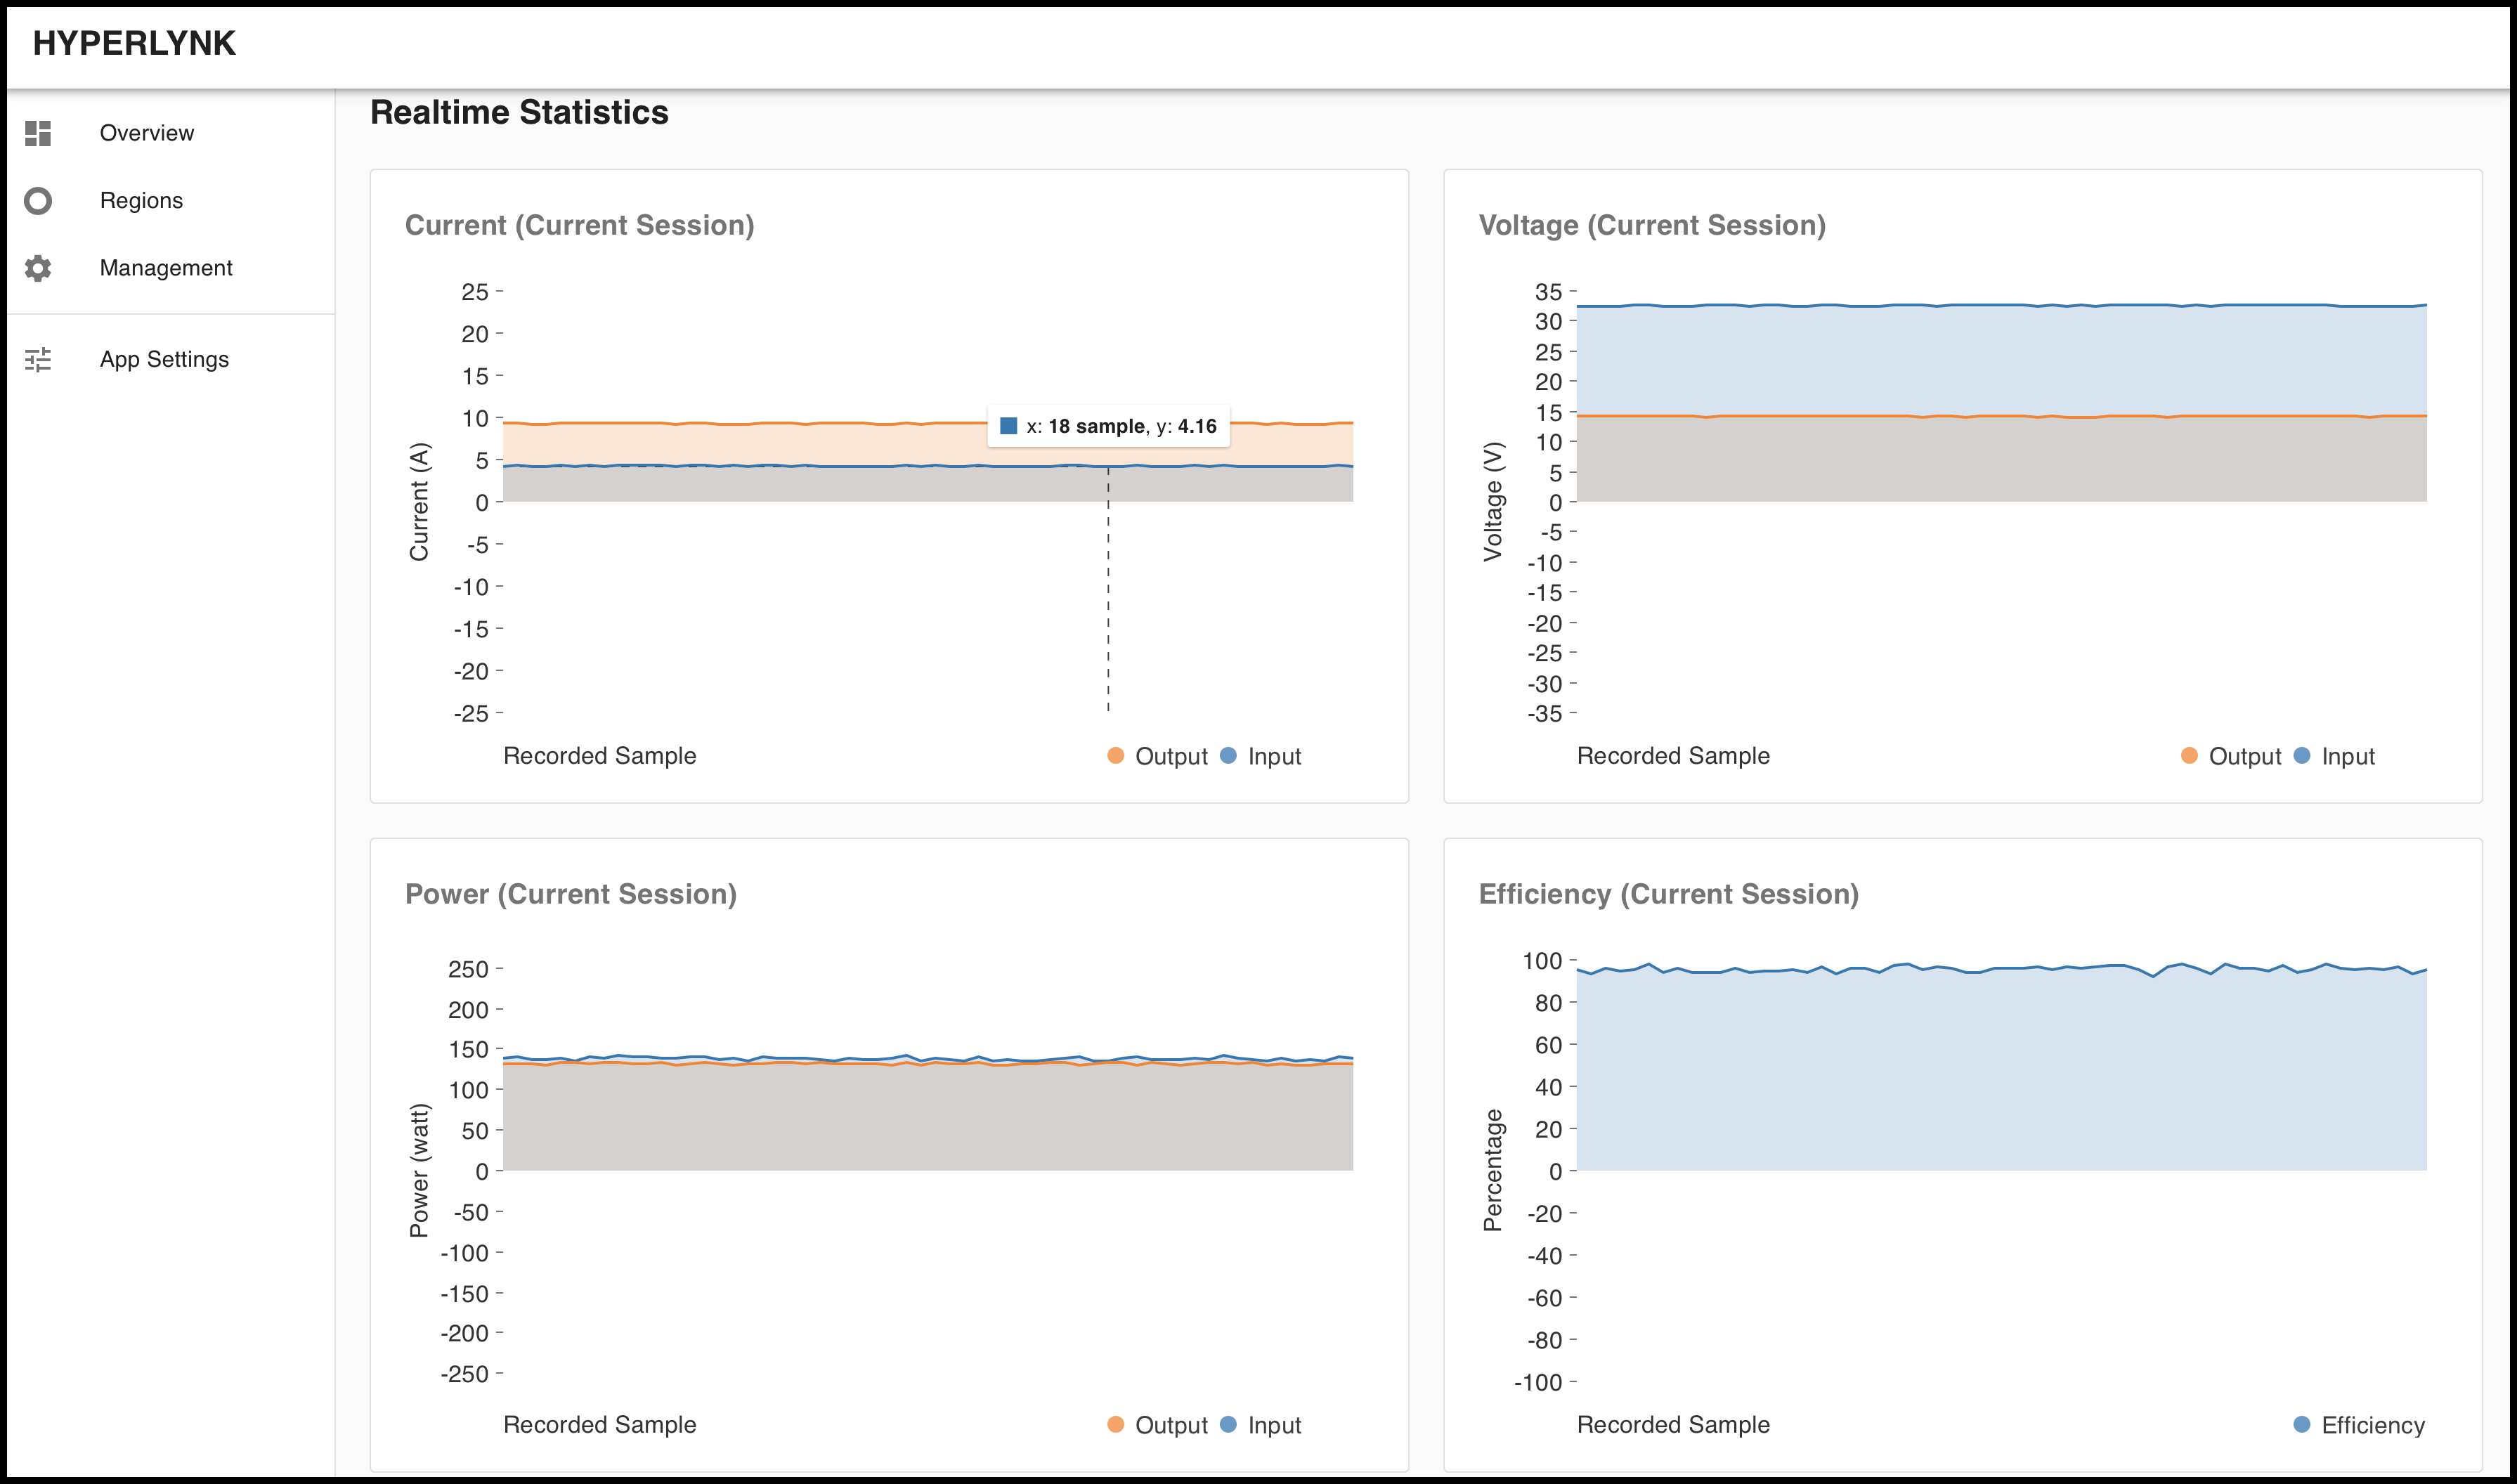
\includegraphics[width=\linewidth]{page3.png}
\caption{The website showing the real-time data.}
\label{fig:page3}
\end{figure}

\begin{figure}[!ht]
\centering
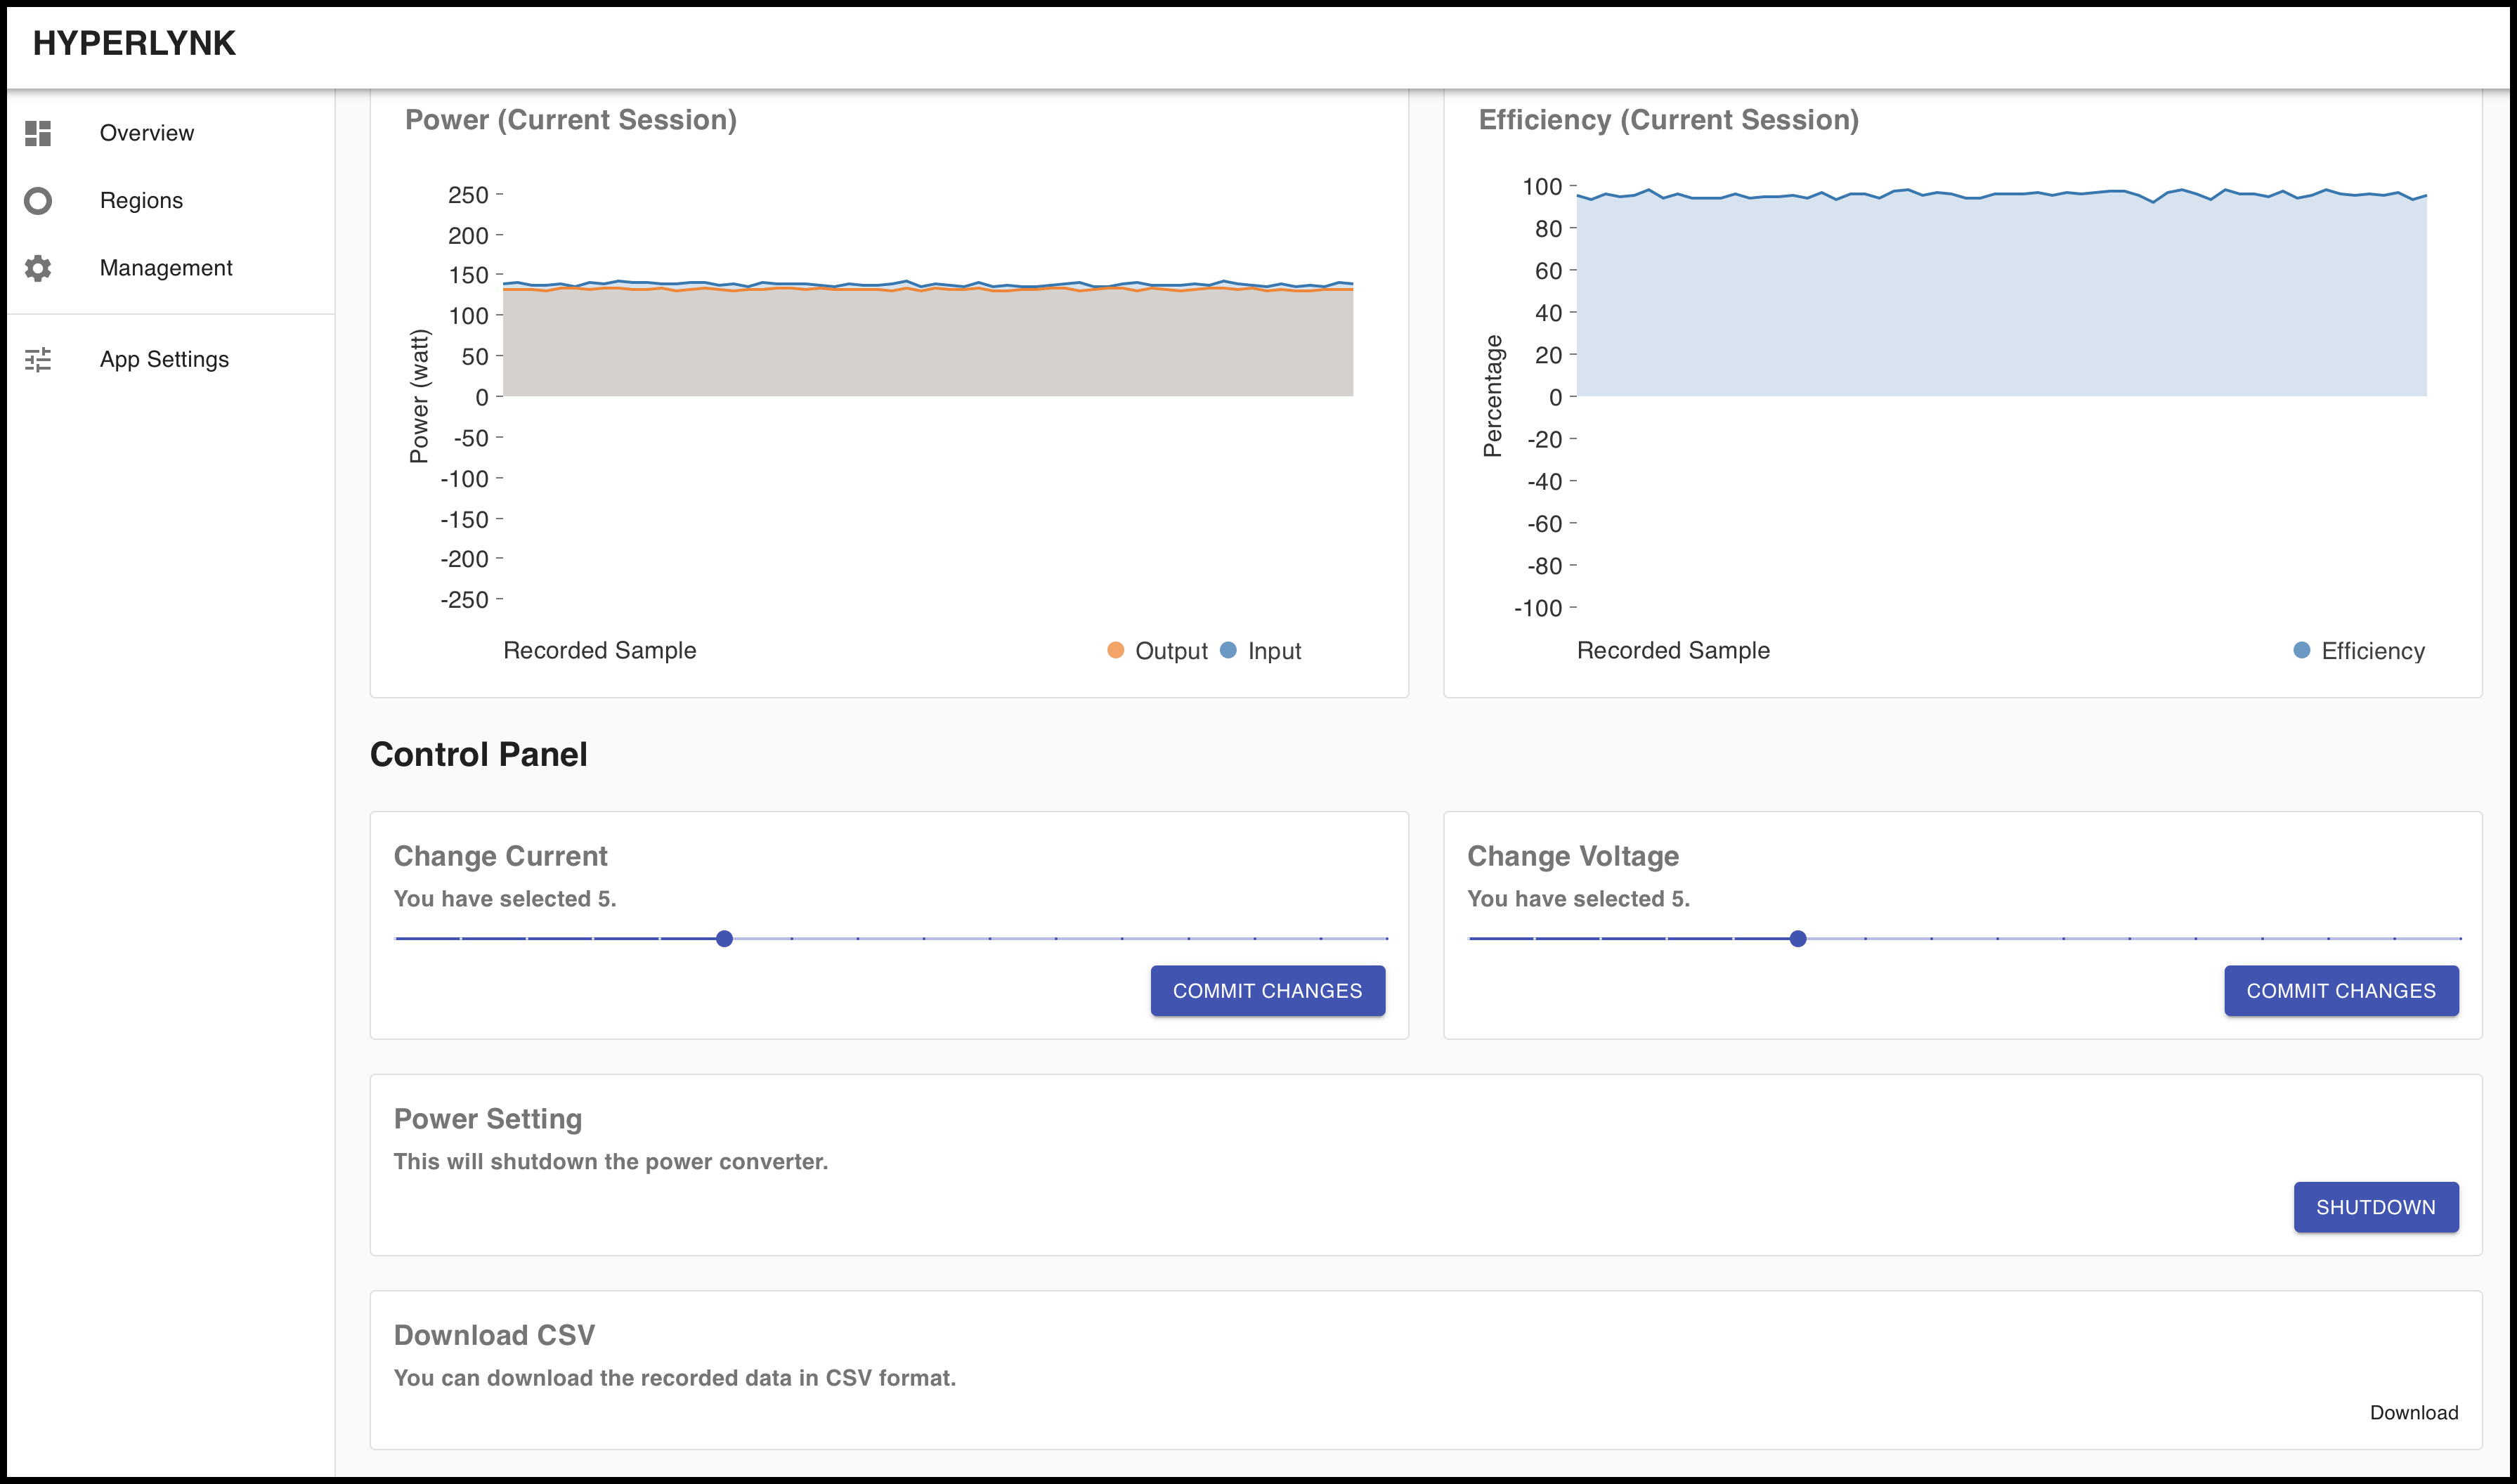
\includegraphics[width=\linewidth]{page4.png}
\caption{The website's control panel.}
\label{fig:page4}
\end{figure}

\begin{figure}[!ht]
\centering
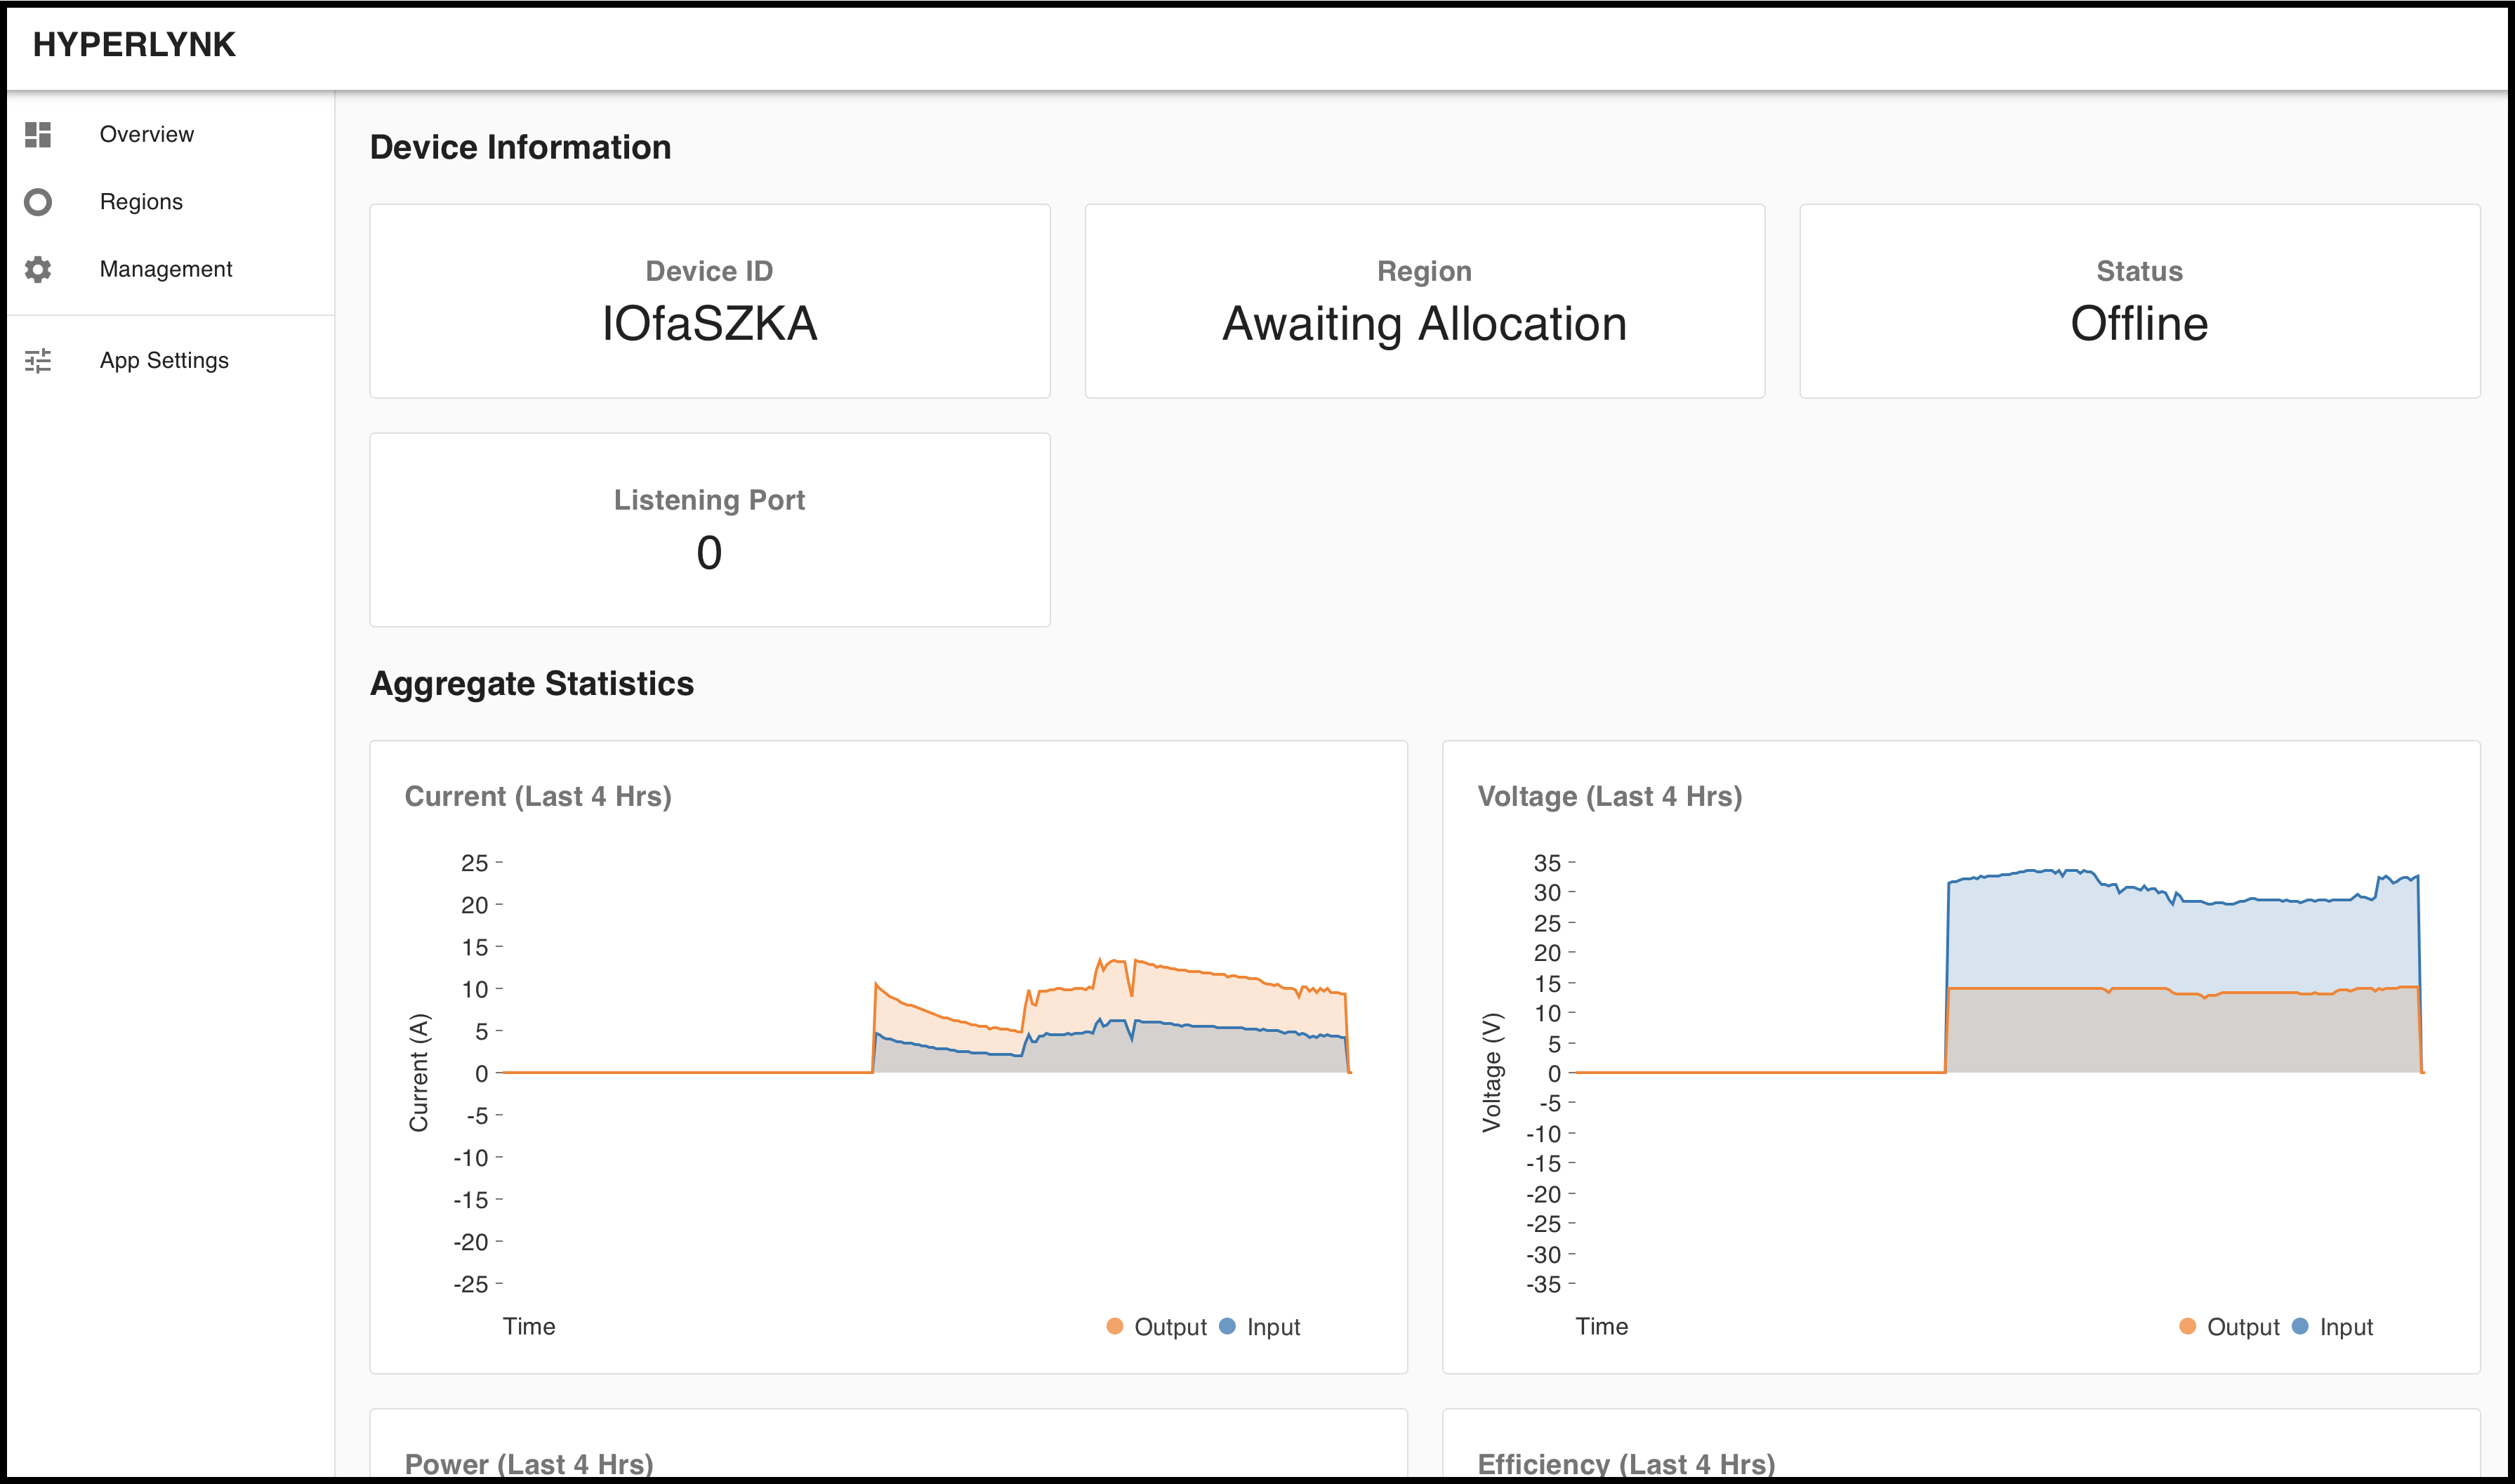
\includegraphics[width=\linewidth]{offline.png}
\caption{The website shows the device is offline.}
\label{fig:offline}
\end{figure}


\begin{figure}[!ht]
\centering
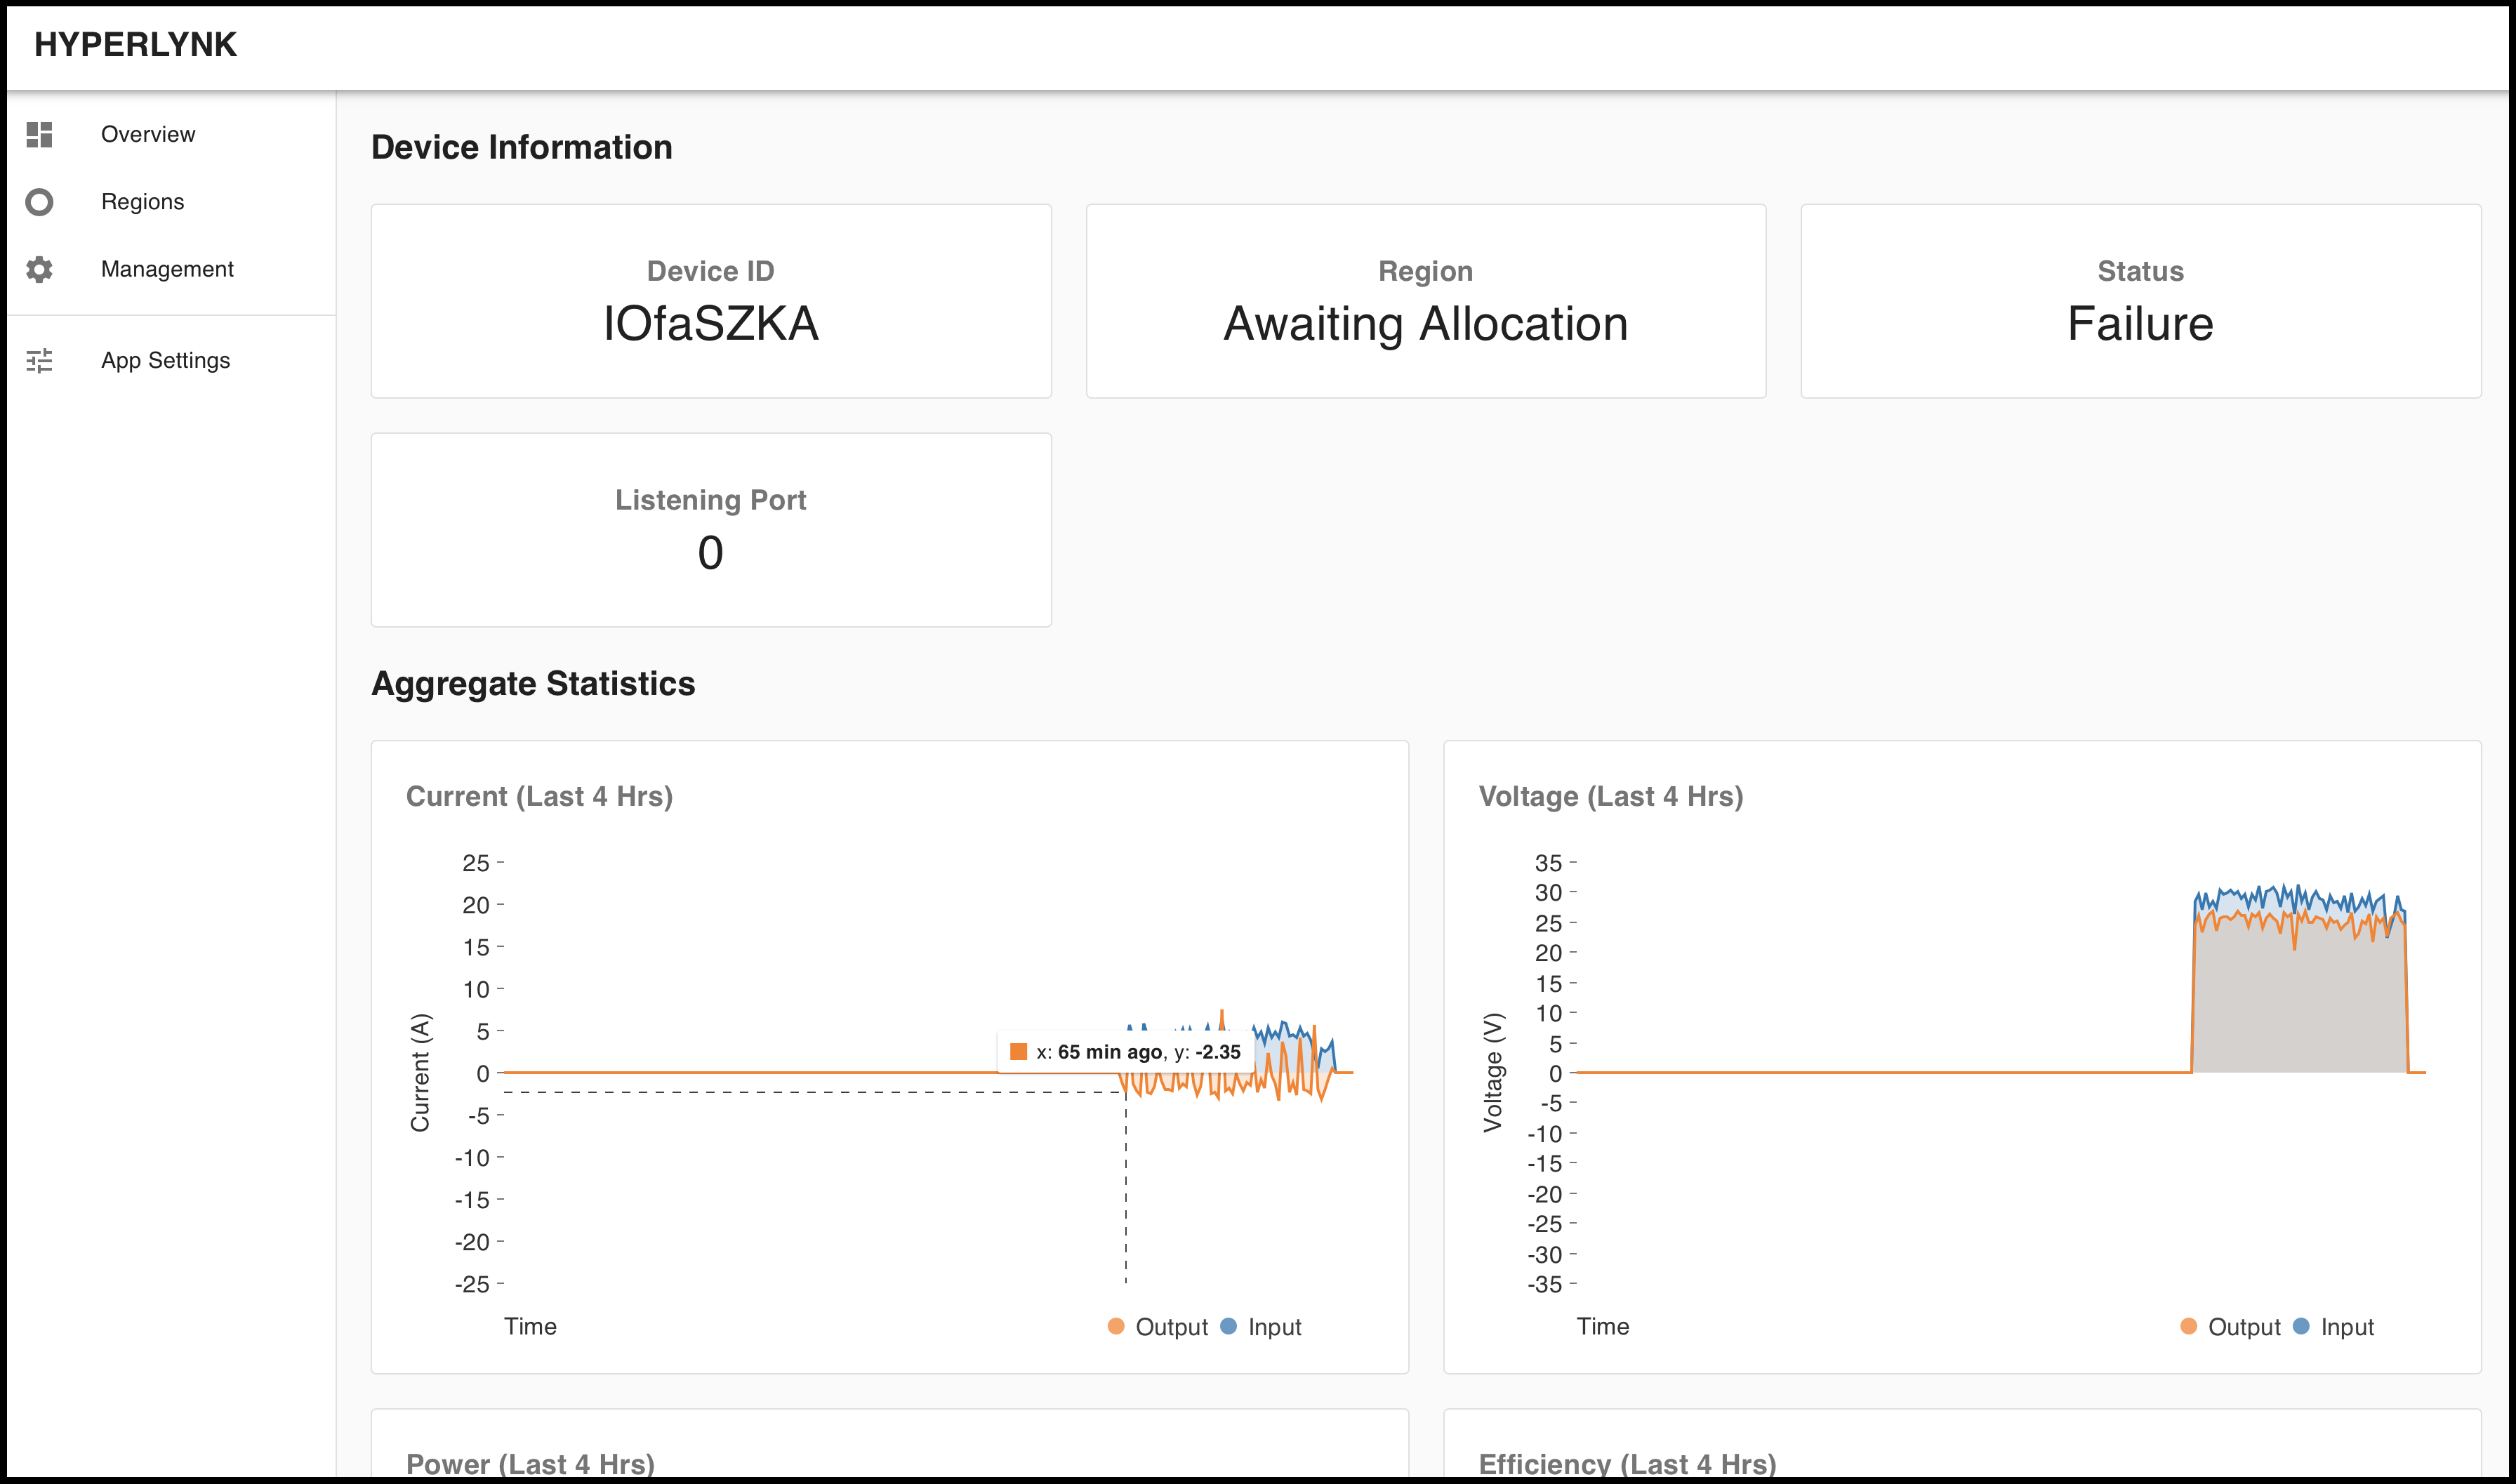
\includegraphics[width=\linewidth]{failure.png}
\caption{The website shows the device has failed.}
\label{fig:failure}
\end{figure}


\end{document}